\documentclass[utf8,a4paper,14pt,simple,floatsection]{eskdtext}

\usepackage[T2A]{fontenc}
\usepackage{mathtext}       % Русские буквы в формулах
\usepackage{caption}        % Позволит подправить заголовки таблиц
\usepackage{longtable}      % Таблицы с переносом на след. страницу 
\usepackage{graphicx}       % Используем графику в документе
\usepackage{textcase}       % Заголовки в ВЕРХНЕМ РЕГИСТРЕ
\usepackage{rotating}       % Поворот текста

% Двухсантиметровый отступ слева перед заголовками таблиц
\captionsetup[table]{%
    labelsep=dash,justification=raggedright,singlelinecheck=false,%
    aboveskip=3mm,belowskip=0mm,margin=2cm}

% Настойка заголовков разделов и подразделов ESKDX
\ESKDsectAlign{section}{Center}
\ESKDsectStyle{section}{\MakeTextUppercase}

\ESKDsectAlign{subsection}{Left}
\ESKDsectStyle{subsection}{}

\ESKDsectAlign{subsubsection}{Left}
\ESKDsectStyle{subsubsection}{}



% Настройки ESKDX
\ESKDgroup{ДГМА}
\ESKDsignature{ДП.05651316.ЭСА-06-1зт.000 ПЗ}
\ESKDtitle{Пояснительная записка}
\ESKDauthor{Ревякин Е. А.}

\begin{document}
    \setlength{\abovedisplayskip}{25pt}
    \setlength{\belowdisplayskip}{25pt}
    \setlength{\abovedisplayshortskip}{25pt}
    \setlength{\belowdisplayshortskip}{25pt} 

    \setcounter{page}{4}

    % Реферат
    \ESKDthisStyle{empty} % Страница без основной надписи
    \section*{Реферат}
    Отчет содержит \ESKDtotal{page} страниц, \ESKDtotal{figure} рисунков, \ESKDtotal{table} таблиц.
    
    Объект изучения -- лабораторно-исследовательский стенд двухмассовой системы электропривода с упругой связью.
    
    Цель исследования -- исследовать систему управления электроприводом стенда.

    В данном отчете было рассмотрено: назначение
    лабораторно исследовательского стенда двухмассовой системы
    электропривода, конструкция стенда, функциональная схема установки,
    принципиальная электрическая схема автономного инвертора напряжений,
    принципиальная электрическая схема системы управления электроприводом,
    принцип действия установки.\\ 

    \MakeTextUppercase{%
        Лабораторно-исследовательский стенд, двухмассовая система, автономный инвертор напряжения, уругие колебания, 
        широтно-импульсная модуляция, привод, преобразователь частоты, асинхронный двигатель.
    }

    \newpage

    % Содержание
    \ESKDthisStyle{formII} % Форма страницы II. Остальные страницы по форме IIa
    \tableofcontents
    \newpage

    % Введение
    \section*{Введение}
\addcontentsline{toc}{section}{Введение}
    В настоящее время, наиболее быстрое развитие получили электроприводы
    двухзвенными преобразователями частоты, выполняемыми на основе автономных
    инверторов напряжения (АИН) или инверторов тока (АИТ). В качестве
    выпрямителя в таких схемах преобразователей используется либо неуправляемые
    выпрямители напряжения или тока, либо относительно новые схемы активных
    выпрямителей напряжения или тока.  Особенностью выходных напряжений АИН
    является пульсирующий характер, который обусловлен несовершенством
    существующих алгоритмов управления ключами АИН, особенно в области малых
    частот.  Улучшить качество выходного напряжения АИН возможно при уменьшении
    периода модуляции с использованием известных алгоритмов широтно-импульсной
    модуляции (ШИМ). Однако это уменьшение ограничено динамическими
    возможностями силовых полупроводниковых ключей и значительным ростом
    дополнительных коммутационных потерь.  Широтно-импульсная модуляция в
    автономном инверторе стала активно применяться вследствие появления
    высокопроизводительных, ориентированных только на задачи электропривода
    микроконтроллеров, которые имеют достаточный набор периферии. Наибольших
    успехов в создании таких микроконтроллеров в конце двадцатого века достигли
    такие известные мировые производители как STM Microelectornics, Freescale,
    Texas Instruments, Siemens, Infineon. Таким образом, программная реализация
    перспективных алгоритмов управления на базе современной микропроцессорной
    техники предоставила ряд новых возможностей для построения более
    качественных систем управления электроприводов. 

    \newpage

    % Общая часть
    \section{Общая часть}

    \subsection{Описание базовой системы стенда исследования упругих колебаний %
        в двухмассовой системе электропривода}
        
        Лабораторно исследовательский стенд  представляет собой
        электромеханическую систему на базе асинхронного двигателя с
        короткозамкнутым ротором (рисунок \ref{fig:general-view}).

        \begin{figure}[h!]
            \center{
                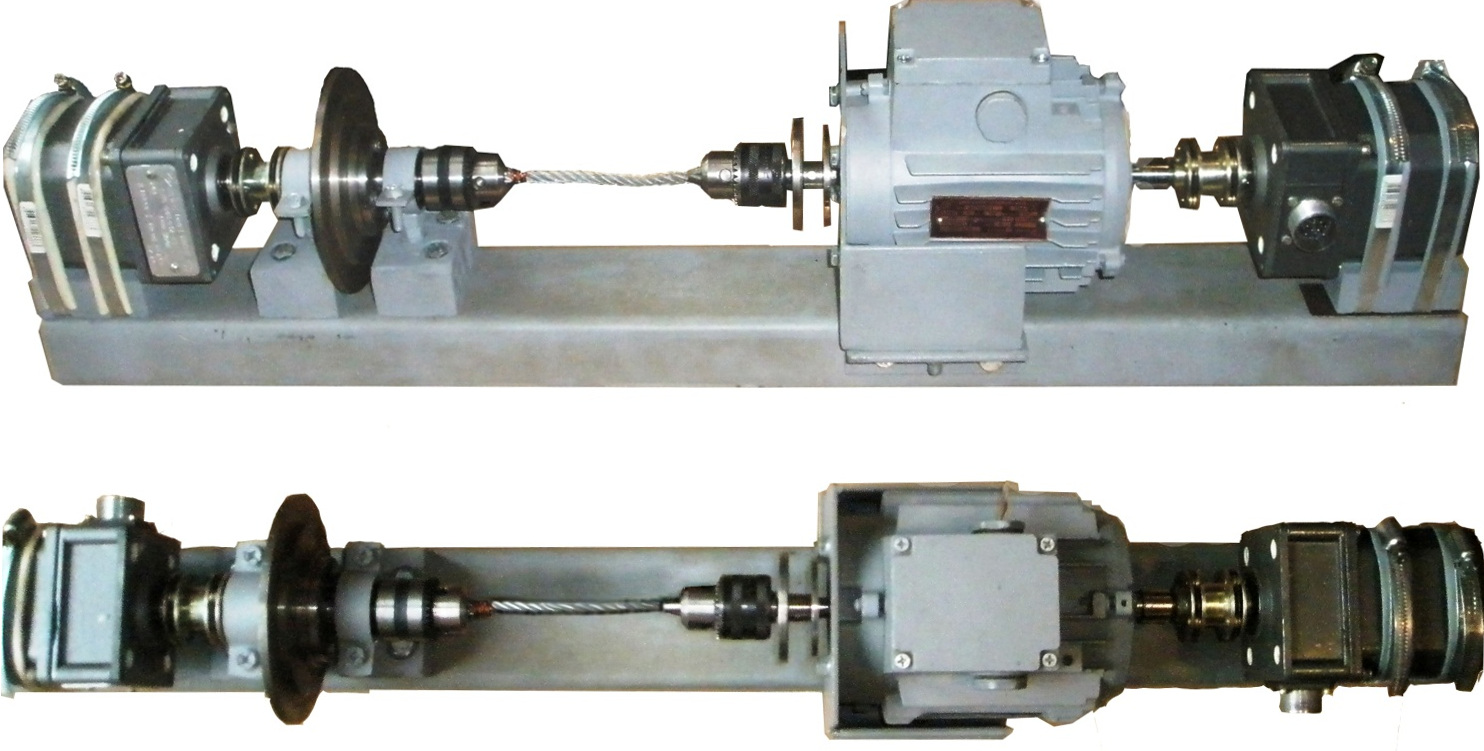
\includegraphics[width=0.8\linewidth]{img/general-view}
            }
            \caption{Общий вид лабораторно исследовательского стенда}
            \label{fig:general-view}
        \end{figure}
        
        В состав стенда входит:
        \begin{itemize}
            \item асинхронный двигатель АИР56А4У3;
            \item 2 фотоэлектрических дискретных датчика перемещения ПДФ-5 с
            разрешающей способностью  600 имп/об;
            \item упругий вал;
            \item силовой блок автономного инвертора напряжения;
            \item блок управления автономным инвертором напряжения.
        \end{itemize}

        Система управления обеспечивает плавный пуск и останов асинхронного
        электродвигателя, с возможностью регулировки частоты вращения. Так же
        система обеспечивает связь с ПК для мониторинга и контроля основных
        параметров.
          
        Питание системы осуществляется от бытовой сети 220 В переменного тока.

    \subsection{Структурная схема системы управления электропривода
        лабораторно - исследовательского стенда}

        Структурная схема системы управления электроприводомлабораторно
        исследовательского стенда представлена на рисунке \ref{fig:struct}.

        \begin{figure}[h!]
            \center{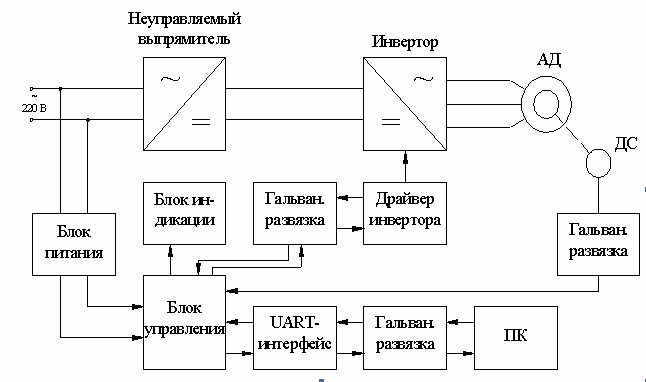
\includegraphics[width=1.0\linewidth]{img/struct}}
            \caption{Структурная схема лабораторно исследовательского стенда}
            \label{fig:struct}
        \end{figure}

        Система частотного электропривода стенда построена по схеме
        двойного преобразования.  Она состит из следующих основных частей:
        звена  постоянного  тока  (неуправляемого выпрямителя), силового
        импульсного инвертора и блока управления.

        Звено постоянного тока состоит из неуправляемого выпрямителя и фильтра.
        Переменное напряжение питающей сети преобразуется в нем в напряжение
        постоянного тока.

        Силовой трехфазный импульсный инвертор состоит из шести транзисторных
        ключей. Каждая обмотка электродвигателя подключается через
        соответствующий ключ к положительному и отрицательному выводам
        выпрямителя. Инвертор осуществляет преобразование выпрямленного
        напряжения в трехфазное переменное напряжение нужной частоты и амплитуды,
        которое прикладывается к обмоткам статора электродвигателя.

        В выходных каскадах инвертора в качестве ключей используются силовые
        MOSFET-транзисторы. По сравнению с тиристорами они имеют более высокую
        частоту переключения, что позволяет вырабатывать выходной сигнал
        синусоидальной формы с минимальными искажениями. 

        Блок управления формирует ШИМ сигналы управления силовым модулем
        инвертора напряжения. В управляющем микроконтроллере блока управления
        програмно реализован алгоритм скалярного управления частотой
        асинхронного двигателя по принципу постоянства отношения напряжения на
        обмотках статора двигателя к частоте этого напряжения (закон управления
        $V/f$).
        
        Все параметры, связанные с управлением приводом, заносятся в память
        контроллера с помощью программирующего устройства или персонального
        компьютера через интерфейс RS232 (модуль UART). Так же через этот
        интерфейс осуществляется мониторинг основных параметров работы системы
        в реальном времени.

        В качестве датчика скорости вращения вала электродвигателя выступает
        дискретный датчик типа ПДФ-5. Датчик представляет собой инкрементный
        квадратурный энкодер оптической системы. Синус-косинусный сигнал с
        выхода датчика поступает в блок управления. Блок управления
        обрабатывает сигнал поступающий от датчика положения и преобразует его
        в значение частоты и направления вращения вала двигателя.

        Блоки гальванической развязки обеспечивают полную гальваническую
        развязку высоковольтных цепей инвертора напряжения с цепями блока
        управления. Тем самым снижая риск поражения электрическим током
        оператора установки. А так же обеспечивая защиту микроконтроллера блока
        управления в случае возникновения аварийных ситуаций во внешних цепях.

        Блок гальванической развязки, расположенный между блоком управления и
        интерфейсом с ПК обеспечивает защиту от разрушения входных цепей
        компъютера разностью потенциалов земель ПК и системы управления.

    \subsection{Технические данные асинхронного двигателя установки}

        В качестве двигателя используется асинхронный двигатель с
        короткозамкнутым ротором модели АИР56А4У3. Технические характеристики
        которого приведены в таблице \ref{table:motor-params}.
         
        На рисунке \ref{fig:motor-overall-dimentions} показаны
        габаритно-установочные и присоединительные размеры двигателя. В таблице
        \ref{table:motor-overall-dimentions} указаны габаритные размеры АД. В
        таблице \ref{table:motor-mounting-dimentions} указаны присоединительные
        размеры двигателя. 
        
        Технические характеристики электродвигателя АИР56АУ3 приведены в
        таблице \ref{table:motor-params}.

        % Габаритно-установочные и присоединительные размеры двигателя
        \begin{figure}[h!]
            \center{%
                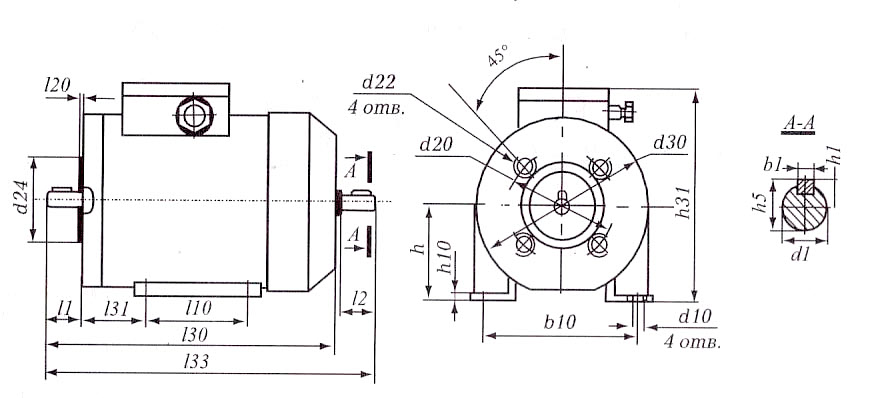
\includegraphics[width=0.8\linewidth]{%
                    img/motor-overall-dimentions}
            }
            \caption{%
                Габаритно-установочные и присоединительные размеры
                двигателя АИР56АУ3
            }
            \label{fig:motor-overall-dimentions}
        \end{figure}
	
        % Габаритные размеры двигателя
        \begin{longtable}{|c|c|c|c|c|c|c|c|}
            \caption{Габаритные размеры двигателя АИР56АУ3
                \label{table:motor-overall-dimentions}}\\
            \hline
            L30 & L33 & d30 & L31 & L1 & L2 & L10 & L20\\
            \hline
            \endfirsthead
            203 & 230 & 80/99 & 141 & 23 & 23 & 71 & 2,5\\
            \hline
        \end{longtable}
        
        % Присоединительные размеры двигателя
        \begin{longtable}{|c|c|c|c|c|c|c|c|c|c|c|c|}
            \caption{Присоединительные размеры двигателя АИР56АУ3
                \label{table:motor-mounting-dimentions}}\\
            \hline
            L31 & d1 & d10 & d20 & d22 & d24 & b1 & b10 & h & h1 & h5 & h10\\
            \hline
            \endfirsthead
            36 & 11 & 5,8 & 85 & М5/М6 & 50/70 & 4 & 90 & 56 & 4 & 12,5 & 7\\
            \hline
        \end{longtable}	

        % Паспортные данные асинхронного двигателя АИР54А4У3
        \begin{longtable}{|c|c|c|c|c|c|c|c|c|c|}
            \caption{Паспортные данные асинхронного двигателя АИР54А4У3
                \label{table:motor-params}}\\
            \hline
            \begin{sideways} Тип двигателя \end{sideways} &
            \begin{sideways} \parbox{6cm}{%
                Номинальная мощность, Вт} \end{sideways} &
            \begin{sideways} \parbox{6cm}{%
                Номинальная  частота вращения, об/мин} \end{sideways} &
            \begin{sideways} \parbox{6cm}{%
                Номинальное напряжение, В} \end{sideways} &
            \begin{sideways} Коэффициент мощности \end{sideways} &
            \begin{sideways} Номинальный ток, А \end{sideways} &
            \begin{sideways} Номинальный момент, Нм \end{sideways} &
            \begin{sideways} \parbox{6cm}{%
                Отношение пускового тока к номинальному} \end{sideways} &
            \begin{sideways} \parbox{6cm}{%
                Отношение максимального момента к номинальному} \end{sideways} &
            \begin{sideways} КПД,\% \end{sideways}\\
            \hline
            \endfirsthead
            АИР56А4У3 & 120 & 1350 & 220 & 0,66 & 0,76 & 0,84 & 5,5 & 2,2 & 63\\
            \hline
        \end{longtable}	

    \subsection{Технические характеристики датчиков перемещения}
        Датчик поворотный дискретный фотоэлектрический ПДФ-5 предназначен
        для преобразования пути (угла поворота) рабочих органов промышленных
        механизмов в число импульсов, а угловой скорости - в частоту следования
        импульсов. 

        Технические характеристики 
        \begin{itemize}
        \item количество выходных каналов - 6. Выходные сигналы (все сигналы
            представлены в прямом и инверсном виде). Две серии импульсов и
            нулевой импульс (один на оборот вала); 
        \item число импульсов в каждой серии на один оборот вала - 600;
        \item Максимальный ток нагрузки каждого канала, мА - 30;
        \item Максимальная частота вращения входного вала - 4000 об/мин;
        \item Номинальное напряжение питания постоянного тока, В - 24;
        \item Номинальное напряжение питания постоянного тока, В - 24;
        \end{itemize}

        Работа выключателя основана на модуляции светового потока,
        направленного от источника излучения через диск с прорезями на
        фотоприемник. При воздействии светового потока на фотоприемник в момент
        прохождения через прозрачный участок диска с выхода выключателя
        снимается сигнал "1". Если световой поток подается на непрозрачный
        участок, и фотоприемник затемнен, на выходе выключателя появляется
        сигнал "0".  
        
        Затем сигнал с фотоприемника усиливается и формируется. После усиления
        по мощности сигнал поступает на разъем, подключаемый к внешней схеме. 

        Датчик (рисунок \ref{fig:encoder}) смонтирован в цилиндрическом литом
        корпусе из алюминиевого сплава, закрытом с двух сторон крышками.
        Подвижный растровый диск укреплен на валу, неподвижный индикаторный
        приклеен к обойме для размещения фотодиодов. Выводы фотодиодов и
        светоизлучателей подпаяны к платам. Элементы электронной схемы
        расположены на трех печатных платах: на двух одинаковых
        усилители-формирователи каналов, на третьей усилитель-формирователь
        нулевого импульса. Цепи выключателя выведены на штепсельный разъем.

        \begin{sidewaysfigure}
            \center{%
                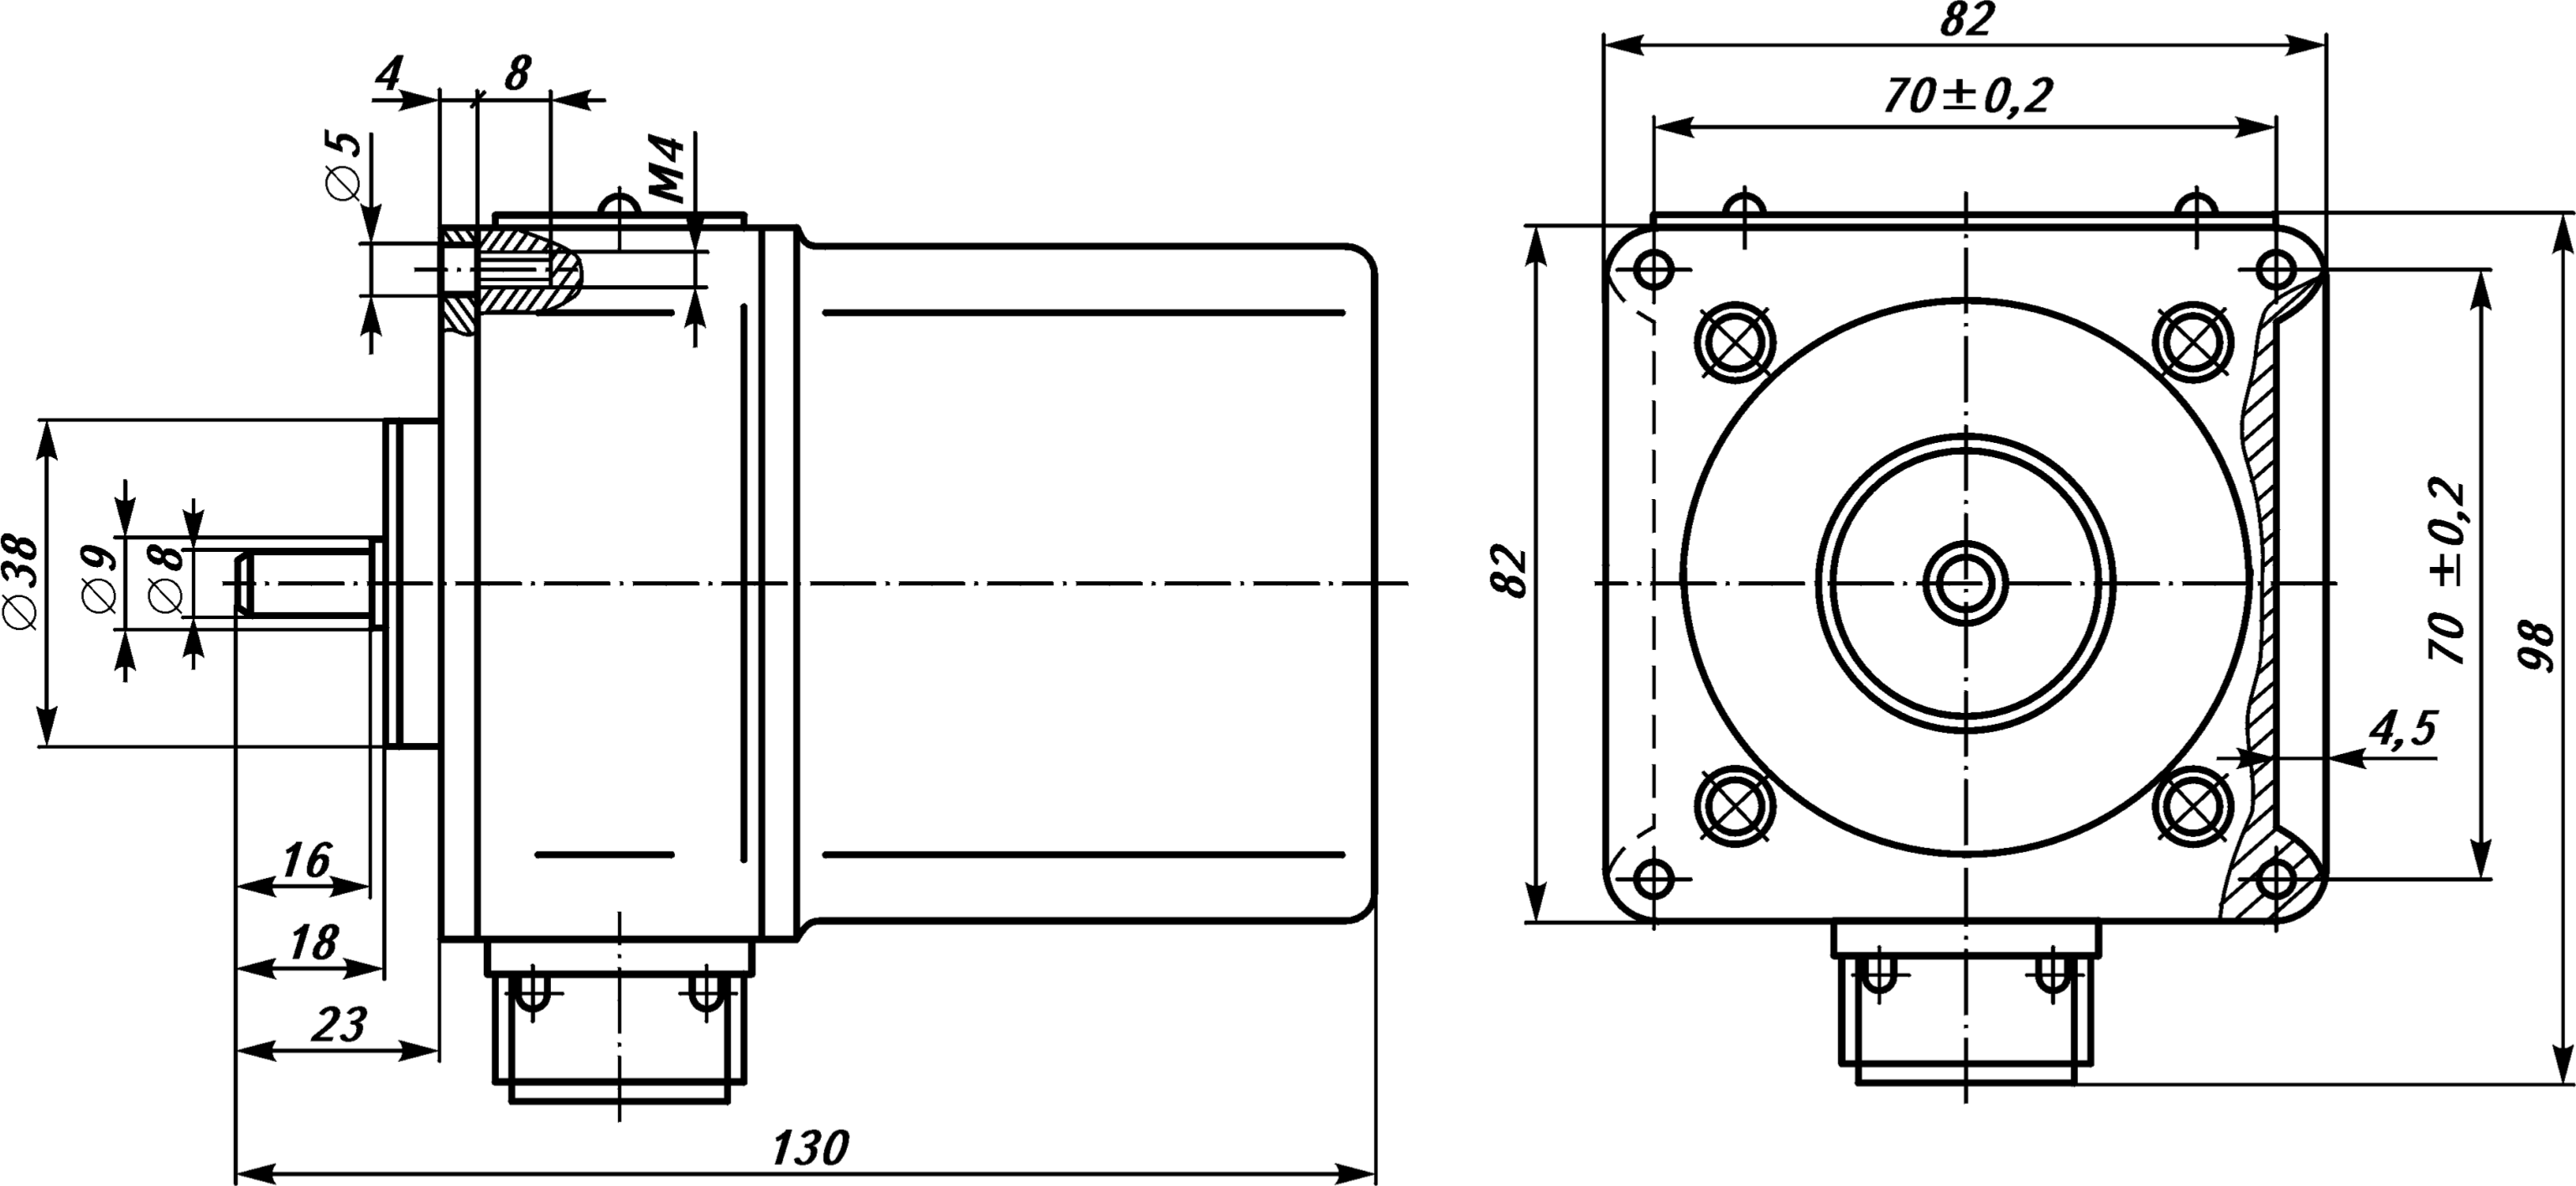
\includegraphics[width=0.8\linewidth]{%
                    img/encoder}
            }
            \caption{%
                Общий вид, габаритные, установочные и присоединительные размеры
                датчика перемещения ПДФ-5
            }
            \label{fig:encoder}
        \end{sidewaysfigure}
        
    \subsection{Электрическая принципиальная схема и описание работы блока
        управления базовой системы}

        Блок управления, схема которого изображена на рисунке
        \ref{fig:mcu-block-schematic} представляет собой МК с набором деталей
        необходимым для его функционирования, а также схемы гальванической
        развязки блока МК с платой драйвера  инвертора, гальванической развязки
        интерфейса датчика скорости и гальванической развязки UART интерфейса
        для связи с ПК.  UART интерфейс обеспечивает соединение с ПК для
        управления и контроля работы электропривода, а также отладки внутренней
        программы МК.
            
        \begin{sidewaysfigure}
            \center{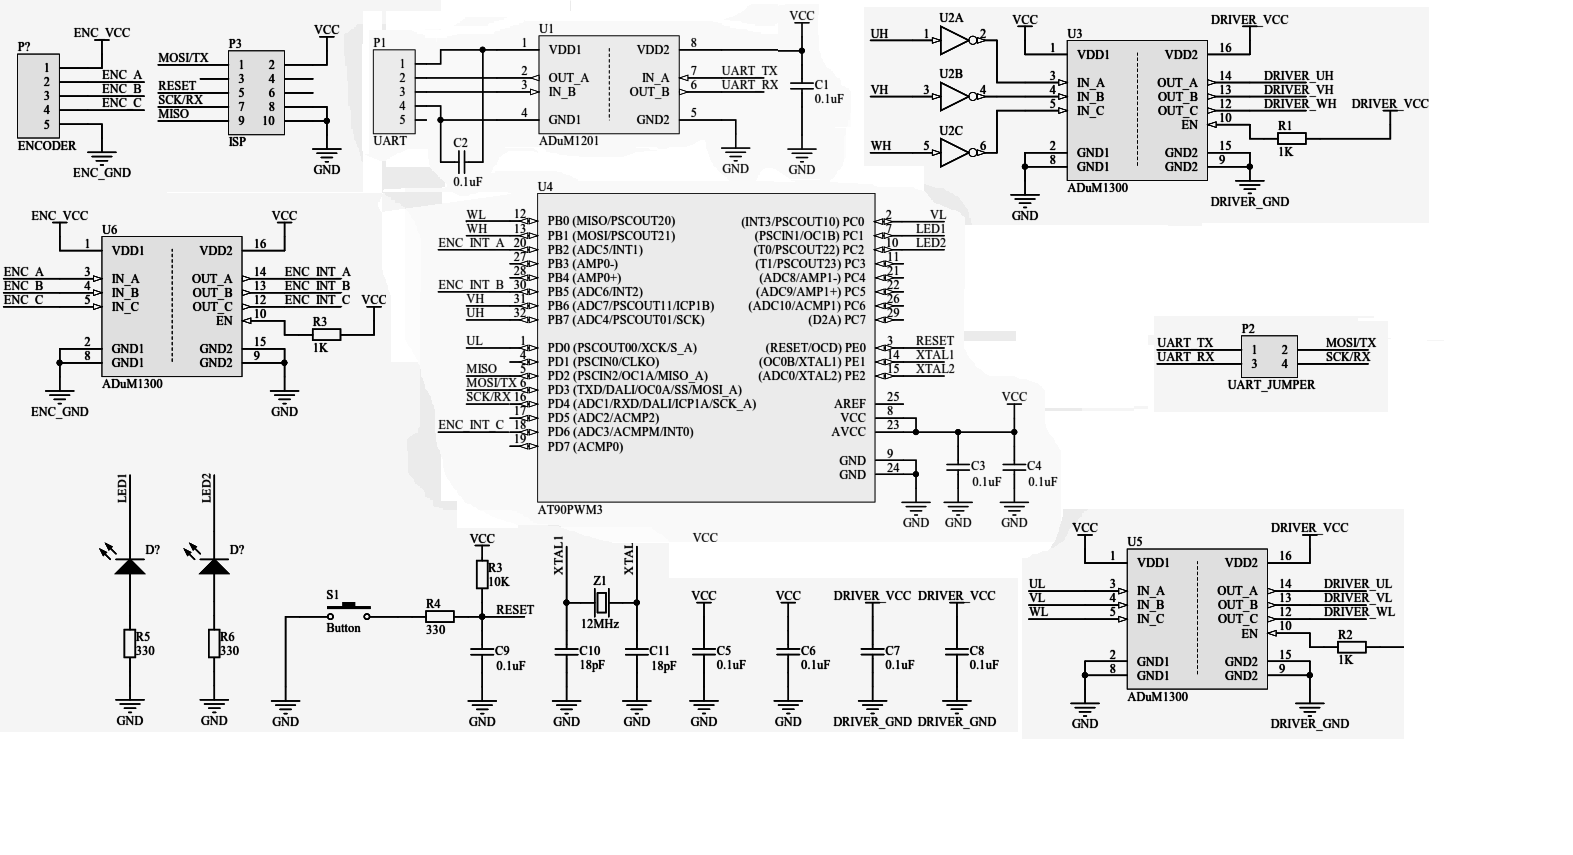
\includegraphics[width=0.8\linewidth]{%
                img/mcu-block-schematic}}
            \caption{Принципиальная электрическая схема блока управления на
                основе МК AT90PWM3}
            \label{fig:mcu-block-schematic}
        \end{sidewaysfigure}
        
        Основой блока управления является микроконтроллер AT90PWM3, структурная
        схема которого показана на рисунке \ref{fig:at90pwm3}.
        
        AT90PWM3 представляет собой экономичный однокристальный
        микроконтроллер, c производительностью до 16 миллионов инструкций в
        секунду. Он предназначен для выполнения функций управления в
        понижающих/повышающих преобразователях постоянного напряжения,
        синхронными электрическими машинами на основе постоянных магнитов,
        трехфазными асинхронными электродвигателями и бесколлекторными
        электродвигателями постоянного тока. 

        \begin{figure}[h!]
            \center{%
                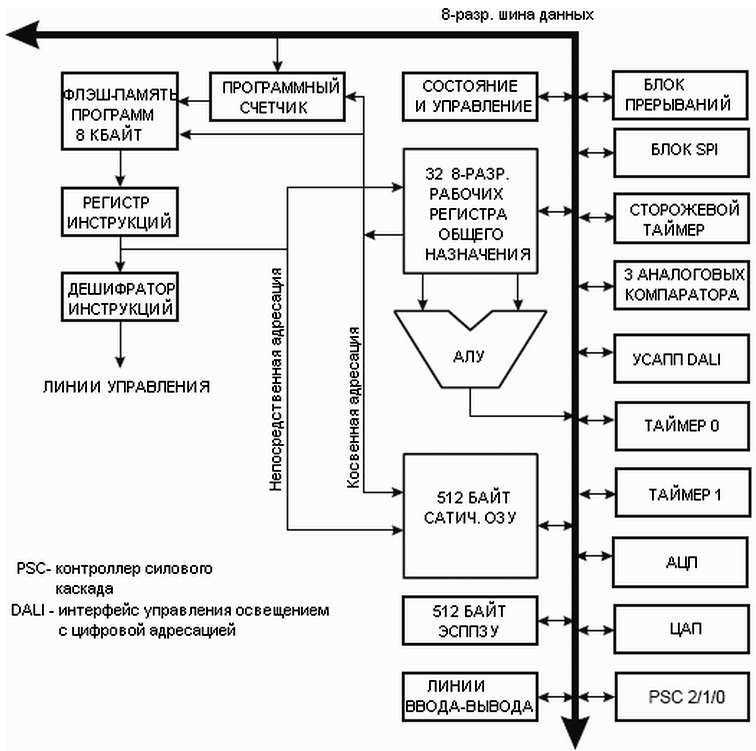
\includegraphics[width=0.8\linewidth]{%
                    img/at90pwm3}
            }
            \caption{Структурная схема микроконтроллера AT90PWM3}
            \label{fig:at90pwm3}
        \end{figure}
        
        Особенностью данного микроконтроллера является наличие блока PSC (Power
        Stage Controller) позволяющего генерировать широтно-модулированный
        сигнал управления тремя полумостами силовых транзисторов. 
        
        Элемент U2 – 74HC04 представляет собой логический инвертор,
        инвертирующий уровни на выходах UH, WH и VH микроконтроллера, так как
        применённая в данной работе ревизия чипа микроконтроллера AT90PWM3
        имеет недоработку состоящую в отсутствии  сдвига фаз на 180 градусов
        между выходными сигналами МК управляющими верхними и нижними ключами
        инвертора.
        
        Микросхемы гальванической развязки U1, U3, U5 и U6 обеспечивают полную
        гальваническую развязку платы блока управления с внешними устройствами,
        тем самым обеспечивают безопасность микроконтроллера в случае
        возникновения аварийной ситуации во внешних цепях, а также в цепях
        связи платы управления с ПК. Микросхема U1 – ADUM1201, представляет
        собой двухканальный двунаправленный цифровой изолятор. U3, U5, U6 –
        ADUM1300 трёхканальные однонаправленные цифровые изоляторы.
        
        Блок микроконтроллера обеспечивает функции плавного пуска, останова,
        реверса электродвигателя, регулировку частоты вращения асинхронного
        электродвигателя с отображением графика её изменения на мониторе
        персонального компьютера.
        
        Внутренняя программа МК реализует разомкнутую систему скалярного
        управления асинхронной машиной переменного тока по принципу постоянства
        отношения $V/f$. Алгоритм работы программы представлен на рисунке
        \ref{fig:old-algorithm}

        \begin{figure}
            \center{%
                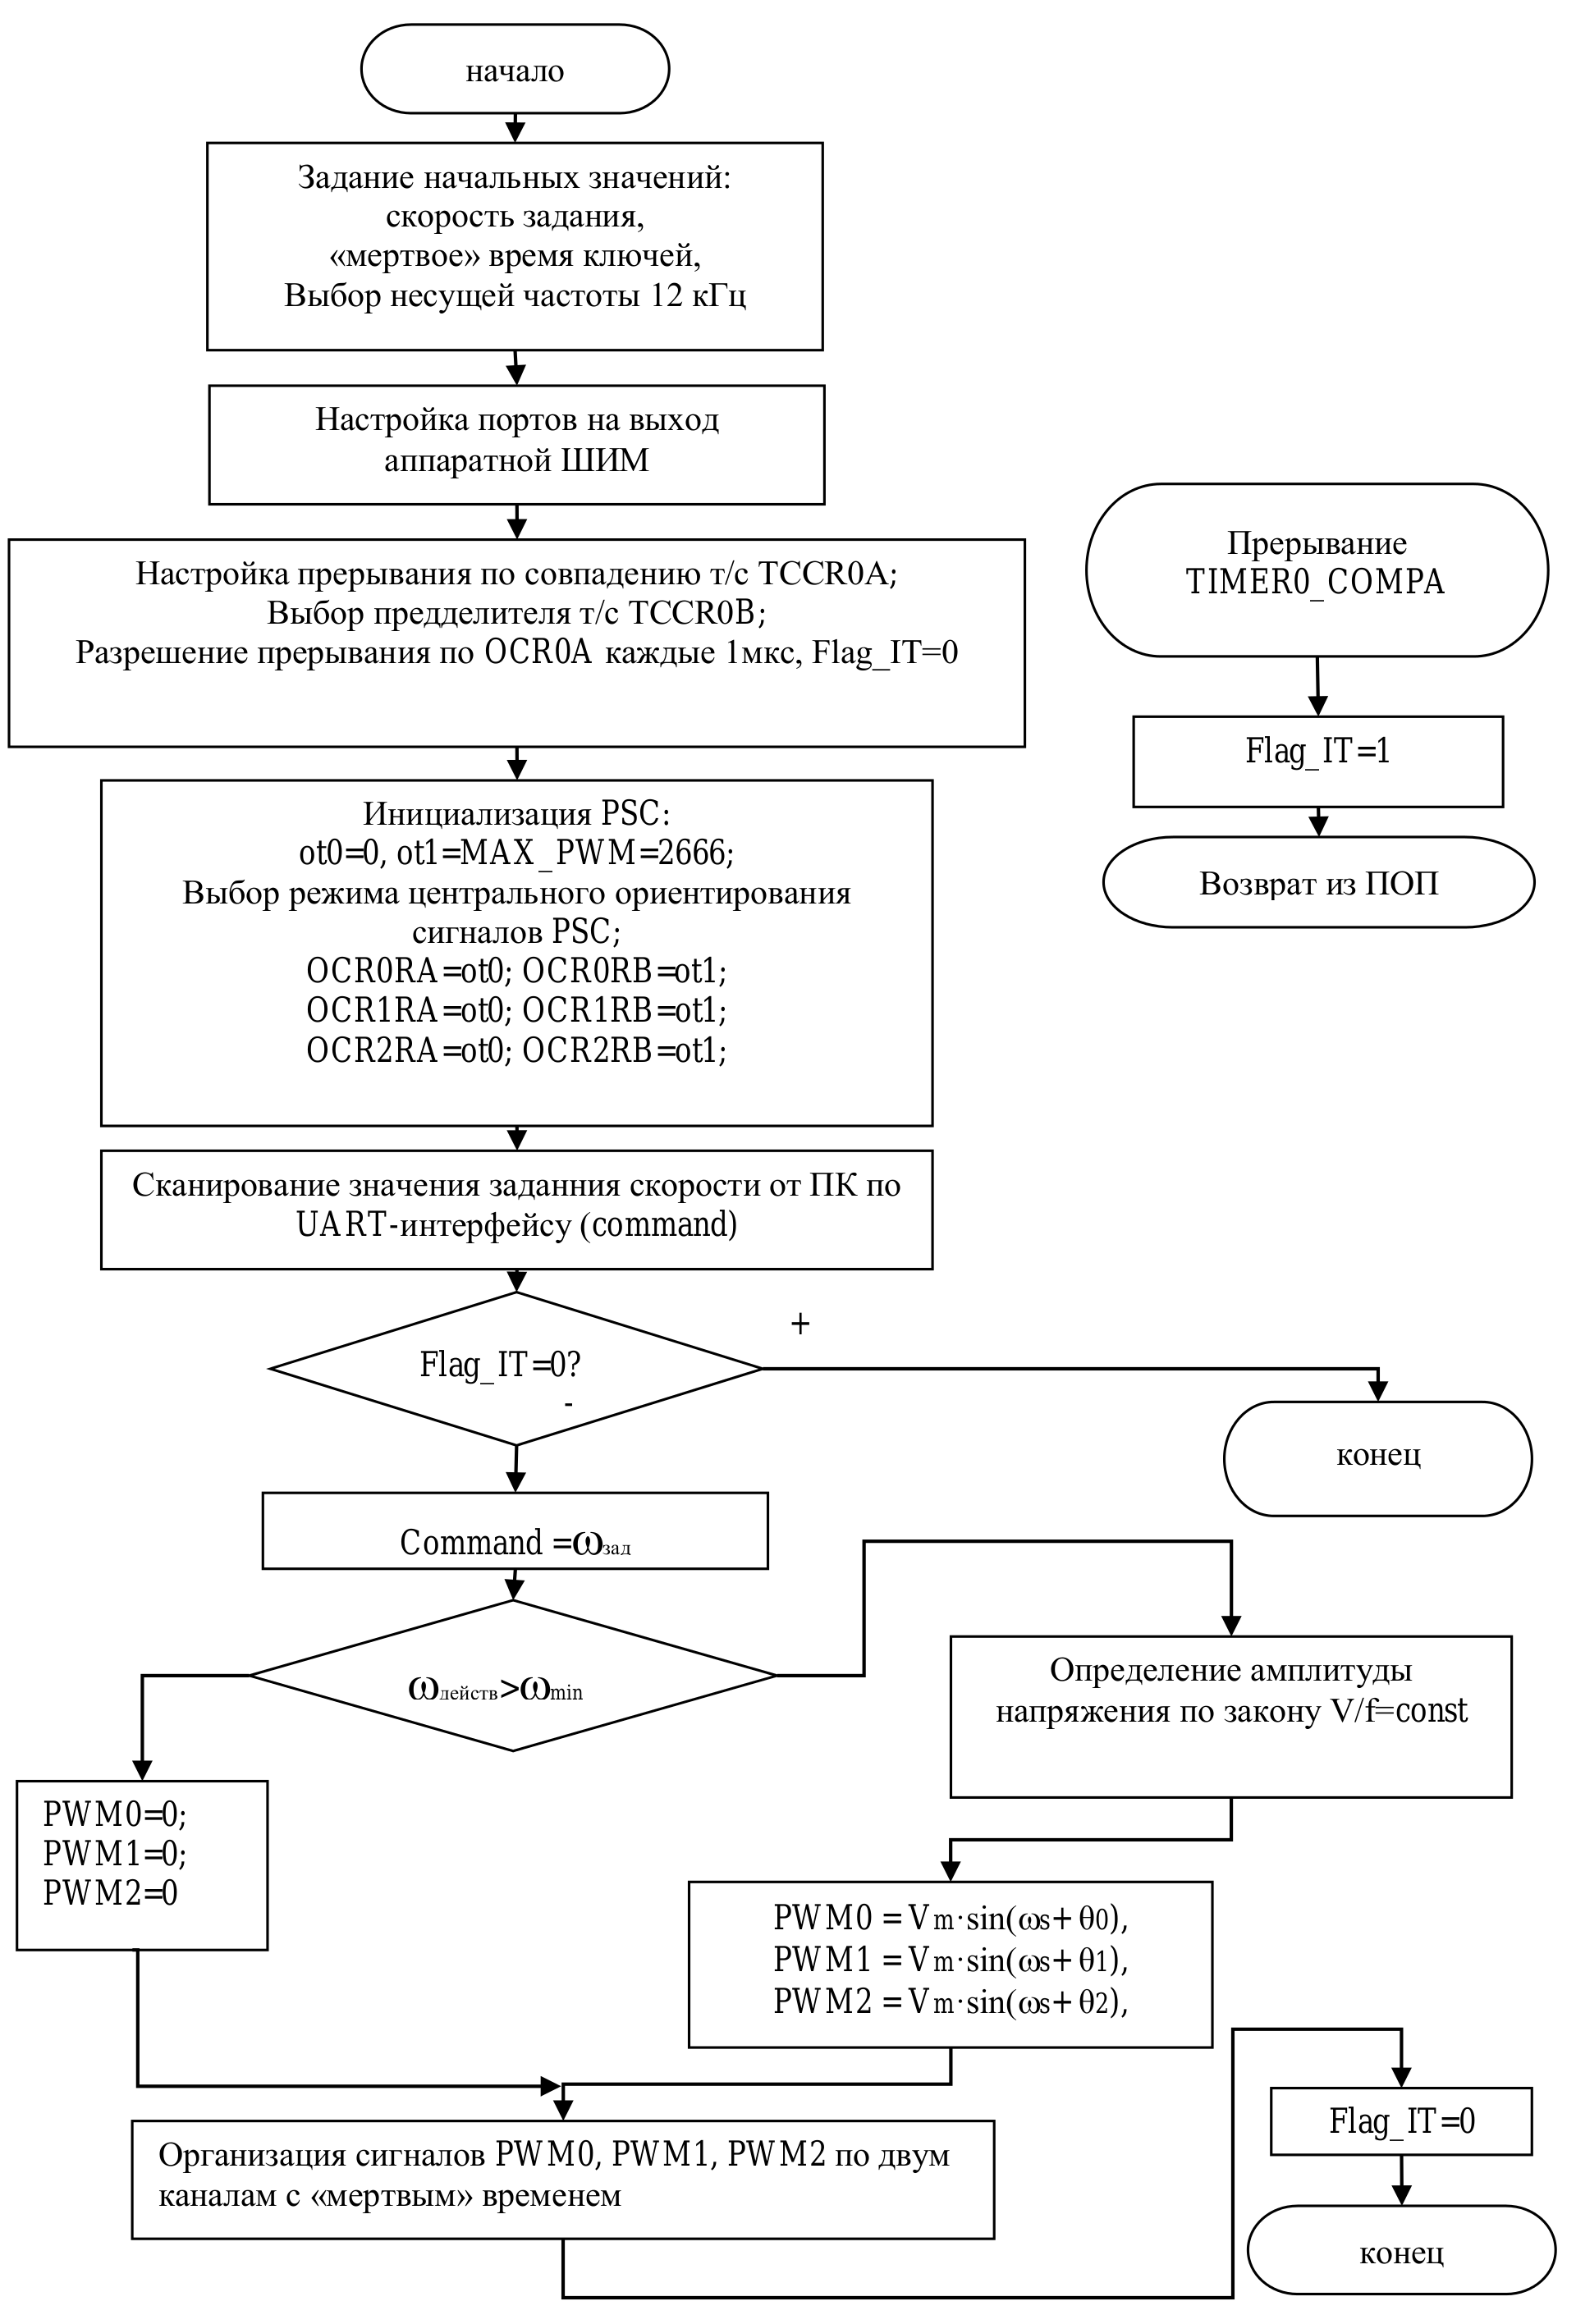
\includegraphics[width=0.9\linewidth]{%
                    img/old-algorithm}
            }
            \caption{Алгоритм работы программы МК базовой системы}
            \label{fig:old-algorithm}
        \end{figure}


    \subsection{Электрическая принципиальная схема и описание работы блока
        инвертора напряжения}

        Принципиальная схема инвертора представлена на рисунке
        \ref{fig:power-block-schematic}. В качестве ключевых транзисторов T1-T6
        выбраны полевые транзисторы типа IRF740.
        
        \begin{sidewaysfigure}
            \center{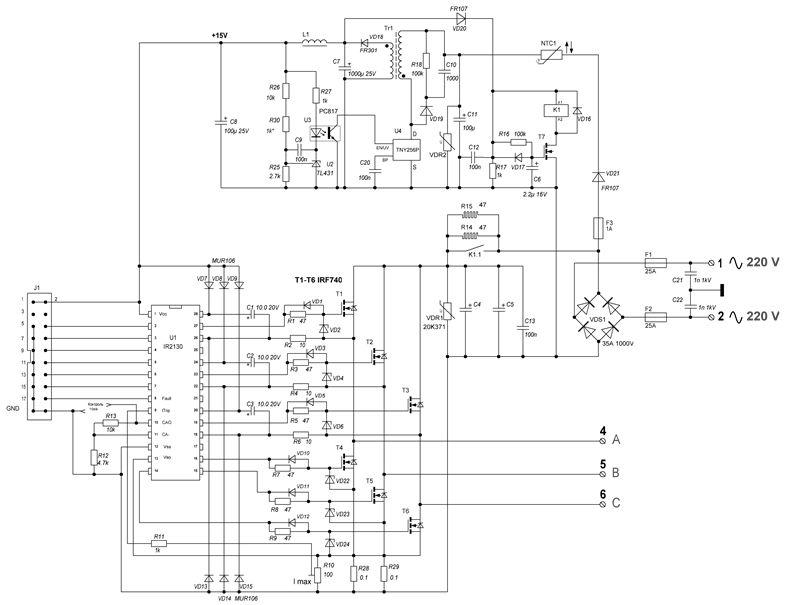
\includegraphics[width=0.8\linewidth]{%
                img/power-block-schematic}}
            \caption{Принципиальная электрическая схема АИН на основе драйвера
                IR2130}
            \label{fig:power-block-schematic}
        \end{sidewaysfigure}
        
        Для непосредственного управления силовыми ключами использована
        специализированная ИМС драйвер трёхфазного моста IR2130, структурная
        схема которой представлена на рисунке \ref{fig:ir2130}. Она
        обеспечивает согласование выходных сигналов блока микроконтроллера с
        силовой частью, а также обеспечивает контроль мёртвого времени силовых
        ключей и защиту выходного каскада от перегрузок по току.

        \begin{figure}[h!]
            \center{%
                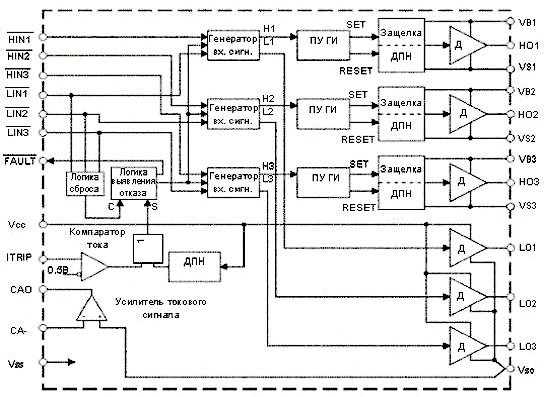
\includegraphics[width=0.8\linewidth]{%
                    img/ir2130}
            }
            \caption{Структурная схема драйвера трехфазного моста IR2130}
            \label{fig:ir2130}
        \end{figure}

        На схеме элементы С21, С22, С11, С12, С14 и VDS1 образуют входной
        сетевой фильтр и входной выпрямитель. Резисторы  R26 и R27 вместе с
        реле K1 и устройством задержки включения на транзисторе Т7 представляют
        собой схему «мягкого» включения инвертора в сеть, необходимую для
        ограничения тока зарядки конденсаторов С11 и С12 и подачи полного
        напряжения питания на транзисторы Т1-Т6 только после полного включения
        ИМС IR2130 и прекращения всех переходных процессов в инверторе, что
        увеличивает надёжность и долговечность работы устройства. 
        
        На микросхеме U4 –TNY256p собран импульсный блок питания,
        обеспечивающий стабилизированное выходное напряжение 15В для питания
        драйвера IR2130.  Микросхема TNY256 представляет собой
        специализированный ШИМ контроллер, предназначенный для создания
        импульсных блоков питания небольшой мощности с минимальным количеством
        навесных компонентов.
        
        Плата автономного инвертора напряжения установлена в корпус от
        импульсного блока питания ПК. Силовые транзисторы выходного каскада
        прикреплены к теплоотводу через изоляционные термопроводящие прокладки.

    \newpage

    % Расчетно-конструкторская часть
    \section{Специальная часть}
        Цель работы – разработать систему управления асинхронным двигателем
        исследовательского стенда электромеханической системы на основе
        микроконтроллера STM32F100RBT6B и трехфазного драйвера силовых
        ключей IR2130. 

        Разработанная система управления должна обеспечивать плавный пуск и
        останов асинхронного электродвигателя, с возможностью регулировки
        частоты вращения. Так же должна обеспечиваться стабилизация частоты
        вращения электродвигателя с помощью обратной связи по скорости. 

        Разрабатываемая система должна обеспечивать связь с ПК для мониторинга
        и контроля основных параметров.

        Питание системы должно осуществляться от бытовой сети 220 В переменного
        тока.

    \subsection{Расчет основных параметров двигателя}
        Пусковой ток
        \begin{gather*}
            I_\text{п} = 5,5 \cdot I_\text{н}.%,\\
            %I_\text{п} = 5,5 \cdot 0,76 = 4,18 \; \text{А}.
        \end{gather*}

        Номинальное скольжение
        \begin{gather*}
            S_\text{н} = \frac{n_0 - n_\text{н}}{n_0}.%,\\
            %S_\text{н} = \frac{1500 - 1350}{1500} = 0,1.
        \end{gather*}

        Критическое скольжение
        \begin{gather*}
            S_\text{кр} = S_\text{н} \cdot
                \left( \lambda_{max} + \sqrt{\lambda_{max}^2 - 1} \right).%,\\
%            S_\text{кр} = 0,1 \cdot
%                \left( 2,1 + \sqrt{2,1^2 - 1} \right) = 0,416.
        \end{gather*}

        Номинальный момент
        \begin{gather*}
            M_\text{н} = \cfrac{P_\text{н}}
                {2\pi \cdot \cfrac{n_\text{н}}{60}}.%,\\
%            M_\text{н} = \frac{120}{2\pi \cdot \cfrac{1350}{60}}
%                = 0,849 \; \text{Н} \cdot \text{м}.
        \end{gather*}

        Максимальный момент двигателя
        \begin{gather*}
            M_{max} = \lambda \cdot M_\text{н}.%,\\
%%%%%%%%            M_{max} = 2,2 \cdot 0,849 = 1,867 \; \text{Н} \cdot \text{м}.
        \end{gather*}

        Сопротивление статора
        \begin{gather*}
            R_s = \frac{\left(\cfrac{U_\text{н}}{\sqrt{3}}\right)
                \cdot (1 - S_\text{н}) \cdot 1,5}{c_1 \cdot
                    \left(1+\cfrac{c_1}{S_\text{кр}}\right) \cdot
                        M_{max} \cdot (P_\text{н} + \Delta P_\text{Т})}.%,\\
       %     R_s = \frac{\left(\cfrac{220}{\sqrt{3}}\right) \cdot (1-0,1)
       %         \cdot 1,5}{1,026 \cdot \left(
       %            1+\cfrac{1,026}{S_\text{кр}}\right) 1,867 \cdot
       %                 (120 + DP_T)} = 0,18 \; \text{Ом}
        \end{gather*}

        Сопротивление ротора
        \begin{gather*}
                R_r = \frac{P_\text{н} + \Delta P_\text{Т}}
                    {3 \cdot (1-S_\text{н}) \cdot i_\text{к}^2
                        \cdot I_\text{н}^2}.%,\\
%                R_r = \frac{P_\text{н} + \Delta P_\text{Т}}
%                    {3 \cdot (1-S_\text{н}) \cdot i_\text{к}^2
%                        \cdot I_\text{н}^2} = 0,15 \; \text{Ом}.
        \end{gather*}

        Расчет индуктивности статора
        \begin{gather*}
            L_s = \frac{\cfrac{U_\text{н}}{\sqrt{3} \cdot
                (2\pi \cdot f \cdot I_\text{н})}}{\sqrt{1 - \cos^2 f}
                    - \cos f \left(\cfrac{S_\text{н}}{S_\text{кр}}\right)}.%,\\
%            L_s = \frac{\cfrac{220}{\sqrt{3}} \cdot
%                (2\pi \cdot 50 \cdot 0,76)}{\sqrt{1 - 0,66^2}
%                    - 0,66 (0,416)} = 0,0043 \; \text{Гн}.
        \end{gather*}

        Формула рассчета индуктивность ротора
        \begin{gather*}
            L_r = L_s.%,\\
%            L_r = 0,0043 \; \text{Гн}.
        \end{gather*}

        Индуктивность намагничивания
        \begin{gather*}
            L_m = L_s - L_{1s}.
            %L_m = L_s - L_{1s} = 0,00382 \; \text{Гн}.
        \end{gather*}

        Конструктивная постоянная
        \begin{gather*}
            C_{1r} = 1+\frac{L_{1s}}{L_m}.
            %C_{1r} = 1+\frac{L_{1s}}{L_m} = 0,0109.
        \end{gather*}

        Вычислим время разгона
        \begin{gather*}
            t_\text{р} = \frac{\omega_\text{н}}{
                \cfrac{M_\text{н}}{j}}.
%            t_\text{р} = \frac{\omega_\text{н}}{
%                \cfrac{M_\text{н}}{j}} = 0,13 \; \text{с}.
        \end{gather*}

        Номинальная угловуя скорость
        \begin{gather*}
            \omega_\text{н} = \frac{2\pi n_\text{н}}{60}.
%            \omega_\text{н} = \frac{2\pi n_\text{н}}{60} 
%                = \frac{2 \cdot 3,14 \cdot 1350}{60} = 141 \; \text{мин}^{-1}.
        \end{gather*}

        Скорость идеального холостого хода
        \begin{gather*}
            \omega_0 = \frac{2\pi n_0}{60}.
%            \omega_0 = \frac{2\pi n_0}{60} 
%                = \frac{2 \cdot 3,14 \cdot 1500}{60} = 157 \; \text{мин}^{-1}.
        \end{gather*}

        Индуктивное сопротивение статора
        \begin{gather*}
            X_s = 2\pi \cdot 50 \cdot L_s.
%            X_s = 2\pi \cdot 50 \cdot L_s
%                = 6,28 \cdot 50 \cdot 0,0043 = 1,35 \text{Ом}.
        \end{gather*}
        
        Индуктивное сопротивление ротора
        \begin{gather*}
            X_r = 2\pi \cdot 50 \cdot L_r.
%            X_r = 2\pi \cdot 50 \cdot L_r
%                = 6,28 \cdot 50 \cdot 0,0043 = 1,35 \text{Ом}.
        \end{gather*}

        \begin{figure}[h!]
            \center{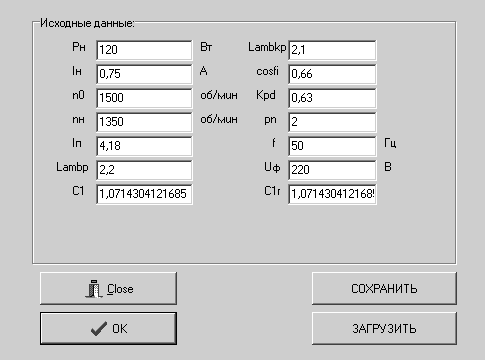
\includegraphics[width=0.6\linewidth]{img/static-scr2}}
            \caption{Входные данные для расчета параметров электродвигателя}
            \label{fig:static-scr2}
        \end{figure}       

        Для рассчета параметров двигателя и построения механических
        характеристик воспользуемся программой STATIC.  На рисунке
        \ref{fig:static-scr2} изображено окно программы со входными данными для
        рассчета.

        Рассчитанные параметры электродвигателя, а также построенные
        механические характеристики показаны на рисунке \ref{fig:static-scr1}.
        Блее детальный вид характеристики, построенной используя однофазную
        схему замещения, приведен на рисунке \ref{fig:motor-mh1}.  А
        механическая характеристика, рассчитанная по формуле Клосса, изображена
        на рисунке \ref{fig:motor-mh2}.

        \begin{figure}[h!]
            \center{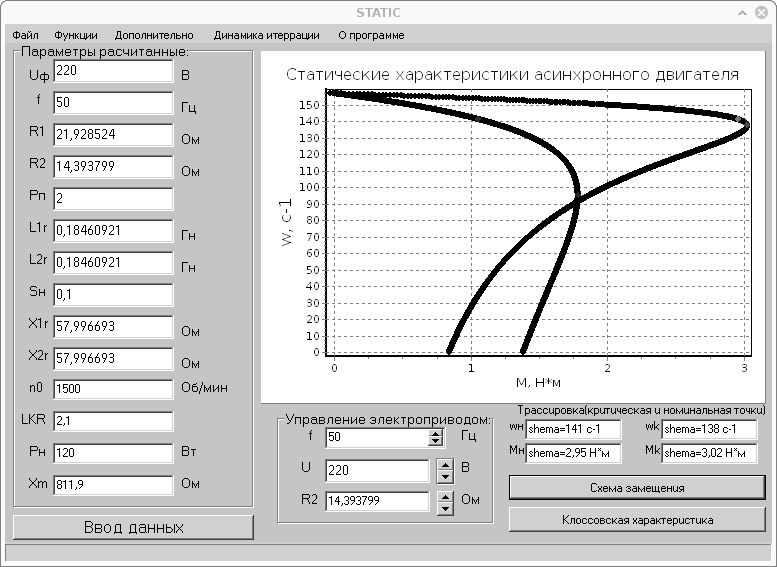
\includegraphics[width=1.0\linewidth]{img/static-scr1}}
            \caption{Окно результатов расчета параметров двигателя}
            \label{fig:static-scr1}
        \end{figure}

        \begin{figure}[h!]
            \center{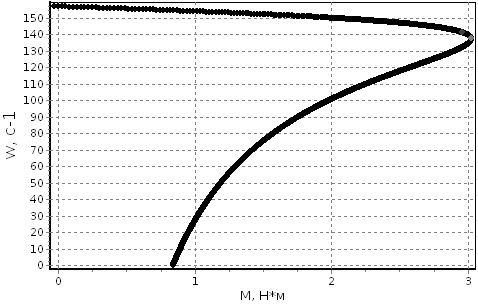
\includegraphics[width=0.6\linewidth]{img/motor-mh1}}
            \caption{Механическая характеристика двигателя, построенная по схеме замещения}
            \label{fig:motor-mh1}
        \end{figure}

        \begin{figure}[h!]
            \center{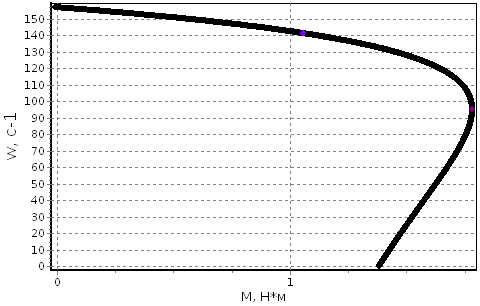
\includegraphics[width=0.6\linewidth]{img/motor-mh2}}
            \caption{Механическая характеристика двигателя, построенная по формуле Клосса}
            \label{fig:motor-mh2}
        \end{figure}

    \subsection{Разработка аппаратной части системы управления автономным
        инвертором напряжения}

%        Разработанная система управления построена на основе отладочного модуля
%        микроконтроллеров серии STM32F100х фирмы ST Microelectronics.

        Блок управления автономным инвертором напряжения реализует
        модулирование ШИМ сигнала управления трехфазным мостом синусоидальным
        сигналом переменной частоты и амплитуды. Амплитуда и частота
        синусоидального сигнала изменяются в соответствии со скалярным законом
        регулирования частоты вращения ротора асинхронного двигателя с
        постоянством отношения $U/f$.

        Принципиальная электрическая схема системы управления АИН представленна
        на рисунке \ref{fig:control-schematic}.

        \begin{sidewaysfigure}
            \center{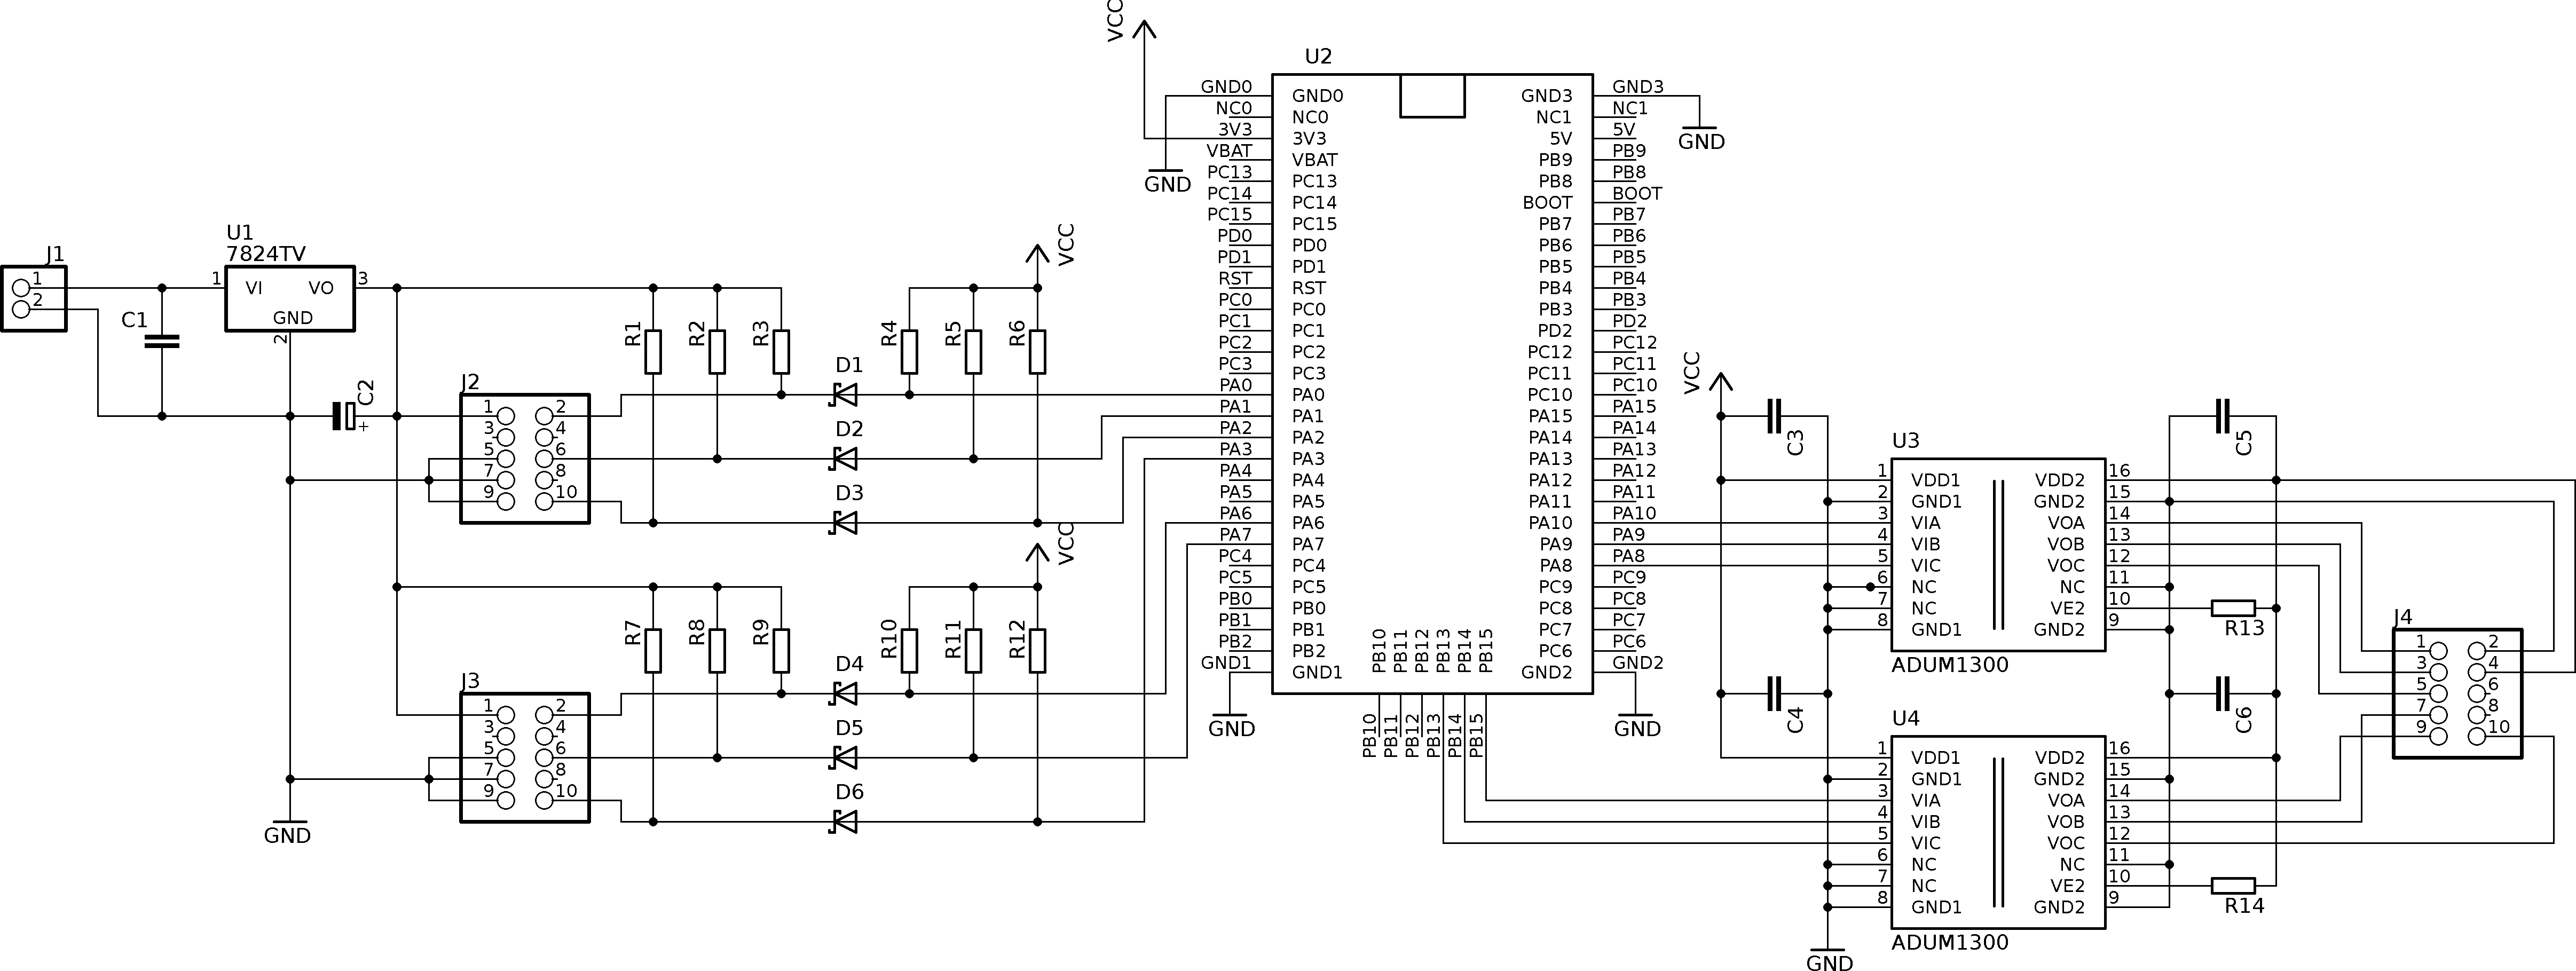
\includegraphics[width=1.0\linewidth]{img/control-schematic}}
            \caption{Принципиальная электрическая схема блока управления АИН}
            \label{fig:control-schematic}
        \end{sidewaysfigure}

        Сигнал управления трехфазным мостом силовых транзисторов АИН снимается
        с выводов PA8, PA9, PA10 (верхние транзизторы моста; фаза A, B и C
        соответственно) и PB13, PB14, PB15 (фаза A, B и C; нижние транзисторы).
        Далее сигнал подается на схему гальванической развязки выполненную на
        двух микросхемах U3 и U4. 
        
        Гальваническая развязка силового блока и блока управления необходима
        так как потенциал общего провода силовой части электропривода может
        иметь значение напряжения питающей сети. Поэтому применением цифровх
        изоляторов с напряжением пробоя болле 2 КВ, обеспечивается защита
        оператора установки от поражения электрическим током, а так же
        буферизация и защита модуля управления от аватийных ситуаций в силовой
        части АИН.

        Конденсаторы С3 - С6 выполняют роль блокировочных, предупреждая броски
        тока в цепяи питания. Резисторы R13 и R14 обеспечивают подтяжку к
        напряжению питания входов разрешения работы цифровых изоляторов.

        Блок управления получает сигналы с двух датчиков скрости через схему
        согласования уровней, выполненную на элементах R1 - R12 и D1 - D6.
        Напряжение питания датчиков скорости снимается с линейного
        интегрального стабилизатора LM7824.

        Конструктивно блок управления выполнен на печатной плате из
        стеклотекстолита толщиной 1,5 мм. Чертеж печатной платы приведен на
        рисунке \ref{fig:control-board-route}. Расоложение элементов -- на
        рисунке \ref{fig:control-board-place}.

        \begin{figure}[h!]
            \center{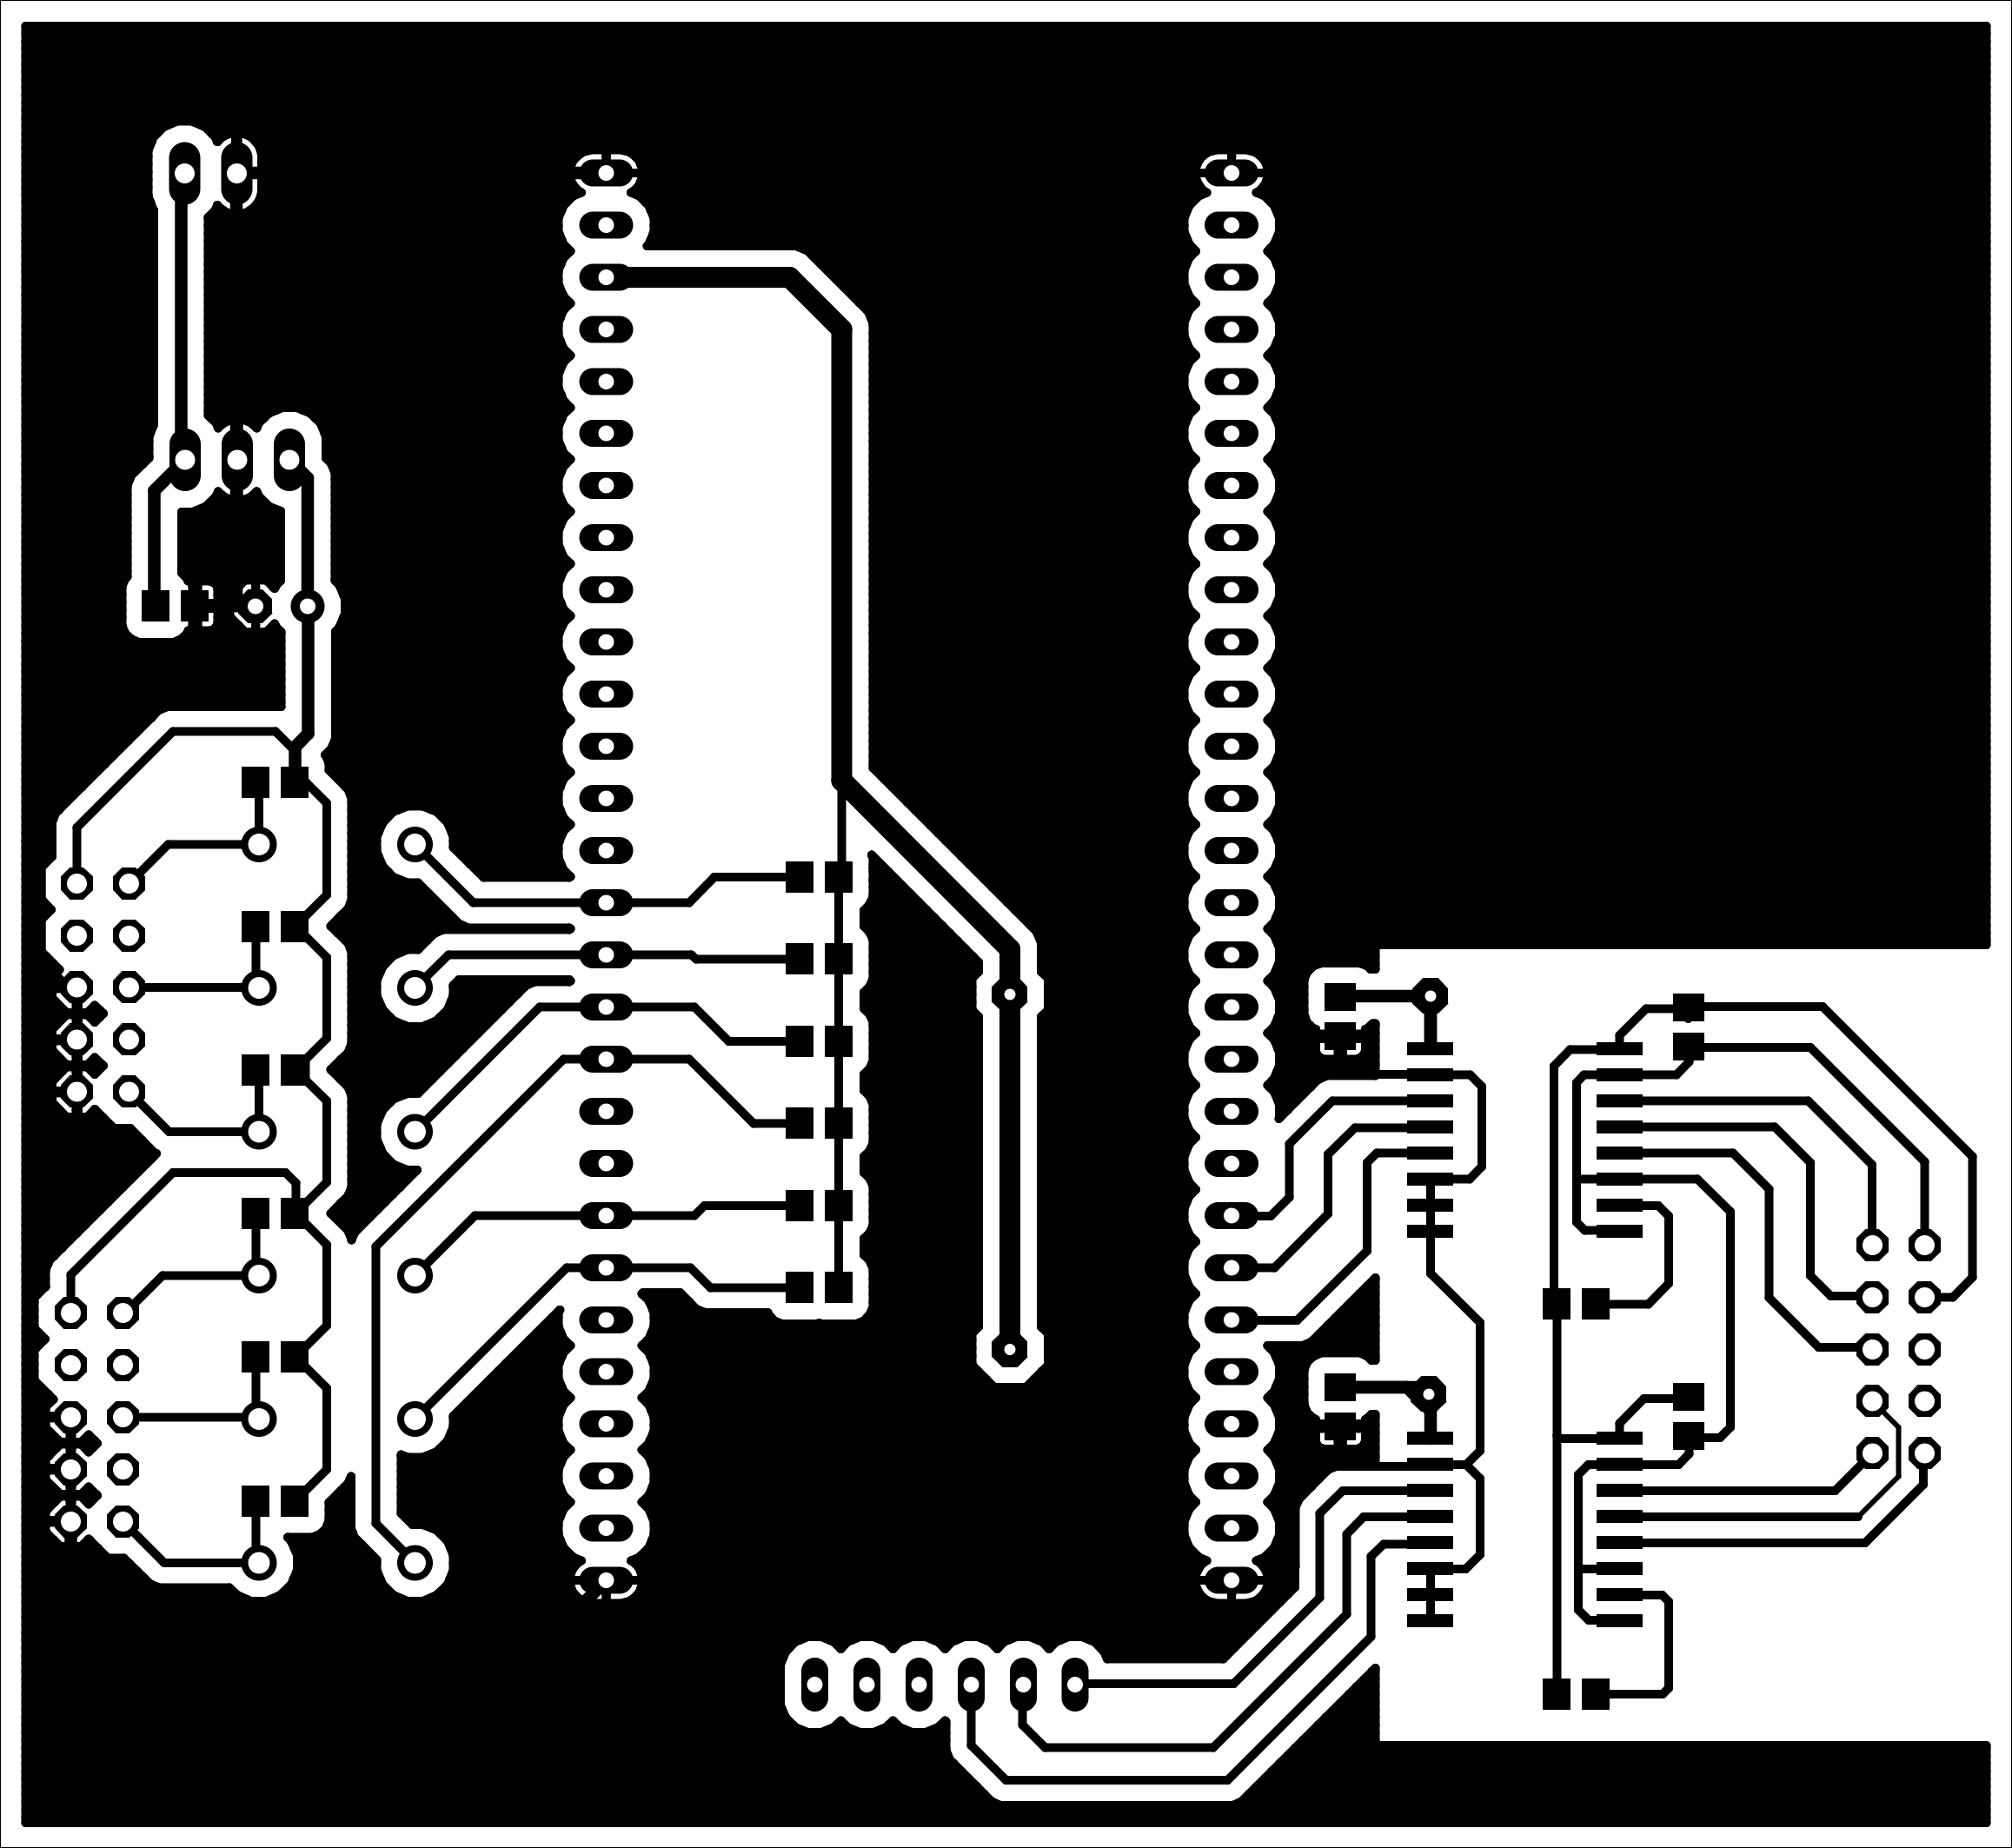
\includegraphics[width=0.8\linewidth]{img/control-board-route}}
            \caption{Чертеж печатной платы блока управления АИН}
            \label{fig:control-board-route}
        \end{figure}

        \begin{figure}[h!]
            \center{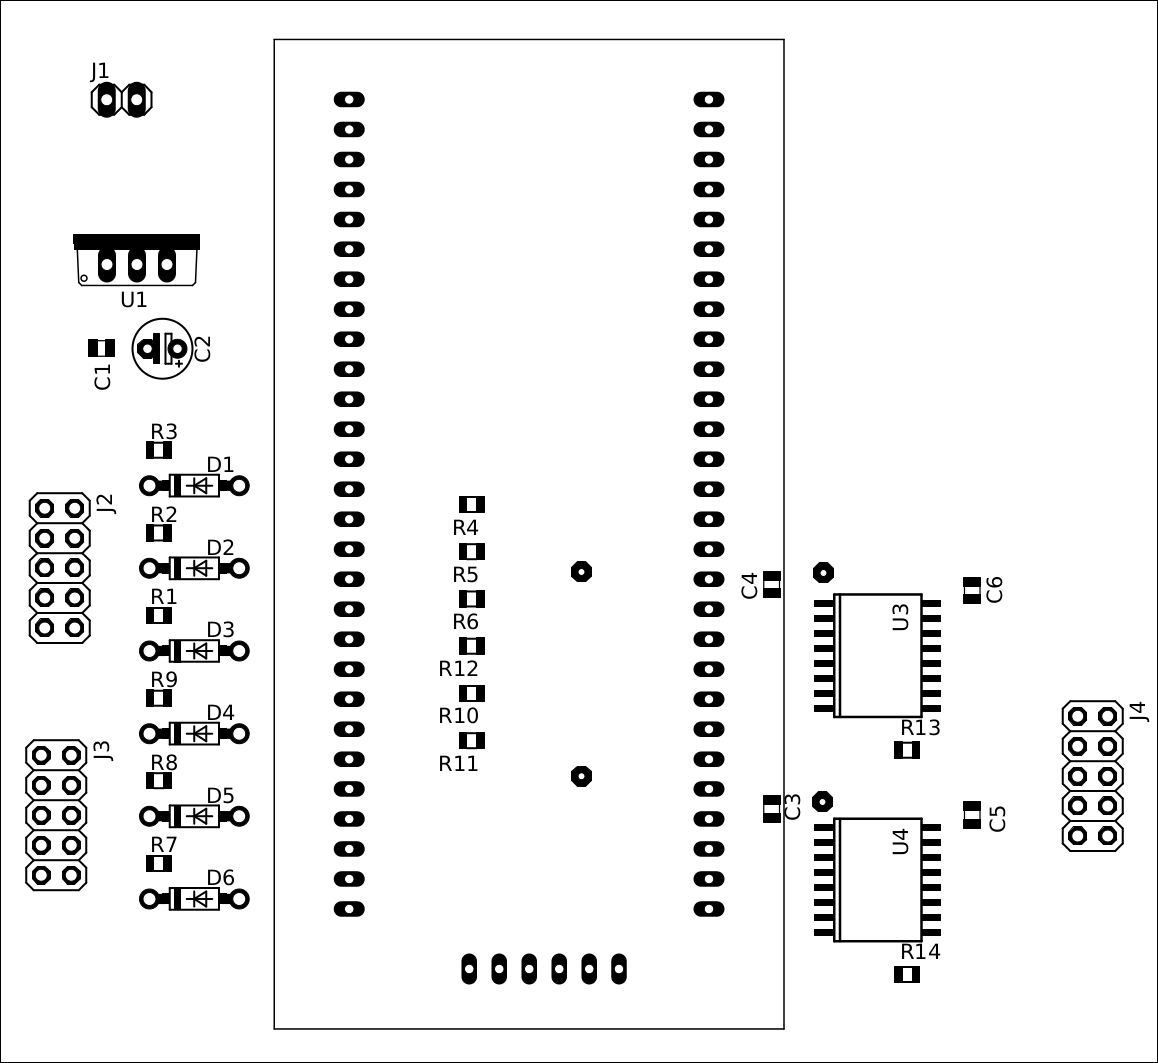
\includegraphics[width=0.8\linewidth]{img/control-board-place}}
            \caption{Схема расположения элементов блока управления АИН}
            \label{fig:control-board-place}
        \end{figure}

        \clearpage
        
    \subsubsection{Описание модуля STM32VLDiscovery}
        STM32VLDiscovery -- встраиваемый модуль с интегрированным\\
        JTAG-отладчиком на базе микроконтроллера STM32F100RBT6B семейства STM32
        Value Line. Работа с платой поддерживается в интегрированной среде
        разработки компаний IAR, Keil, Atollic, а также свободным набором
        компиляторов GNU Compiler Collection.

        Установленный микроконтроллер в 64-выводном корпусе LQFP работает на
        частоте 24 МГц. Плата имеет разъем расширения, который позволяет
        подключать ее к другим отладочным платформам для более глубокого
        анализа работы периферии микроконтроллера или к макетным платам для
        прототипирования.

        Установленный на плате отладчик/программатор ST-Link, может
        использоваться как для внутрисхемного программирования встроенного
        микроконтроллера так и в качестве отдельного устройства.

        Отличительные особенности:
        \begin{itemize}
            \item на плате имеется внутрисхемный отладчик/программатор ST-Link;
            \item USB интерфейс ко встроенному отладчику;
            \item переключатель для использования платы в качестве отдельного
                устройства ST-Link;
            \item питание возможно от USB интерфейса или от внешнего источника; 
            \item два светодиода индикации состояния;
            \item два пользовательских светодиода, пользовательская кнопка,
                кнопка \\ <<Сброс>>;
            \item коннектор расширения – доступны все линии ввода/вывода
                микроконтроллера, может использоваться для подключения к
                макетной плате или другой отладочной системе.
        \end{itemize}

        Внешний вид, расположение элементов и размеры модуля приведены на
        рисунке \ref{fig:stm32vldiscovery}.

        \begin{sidewaysfigure}
            \center{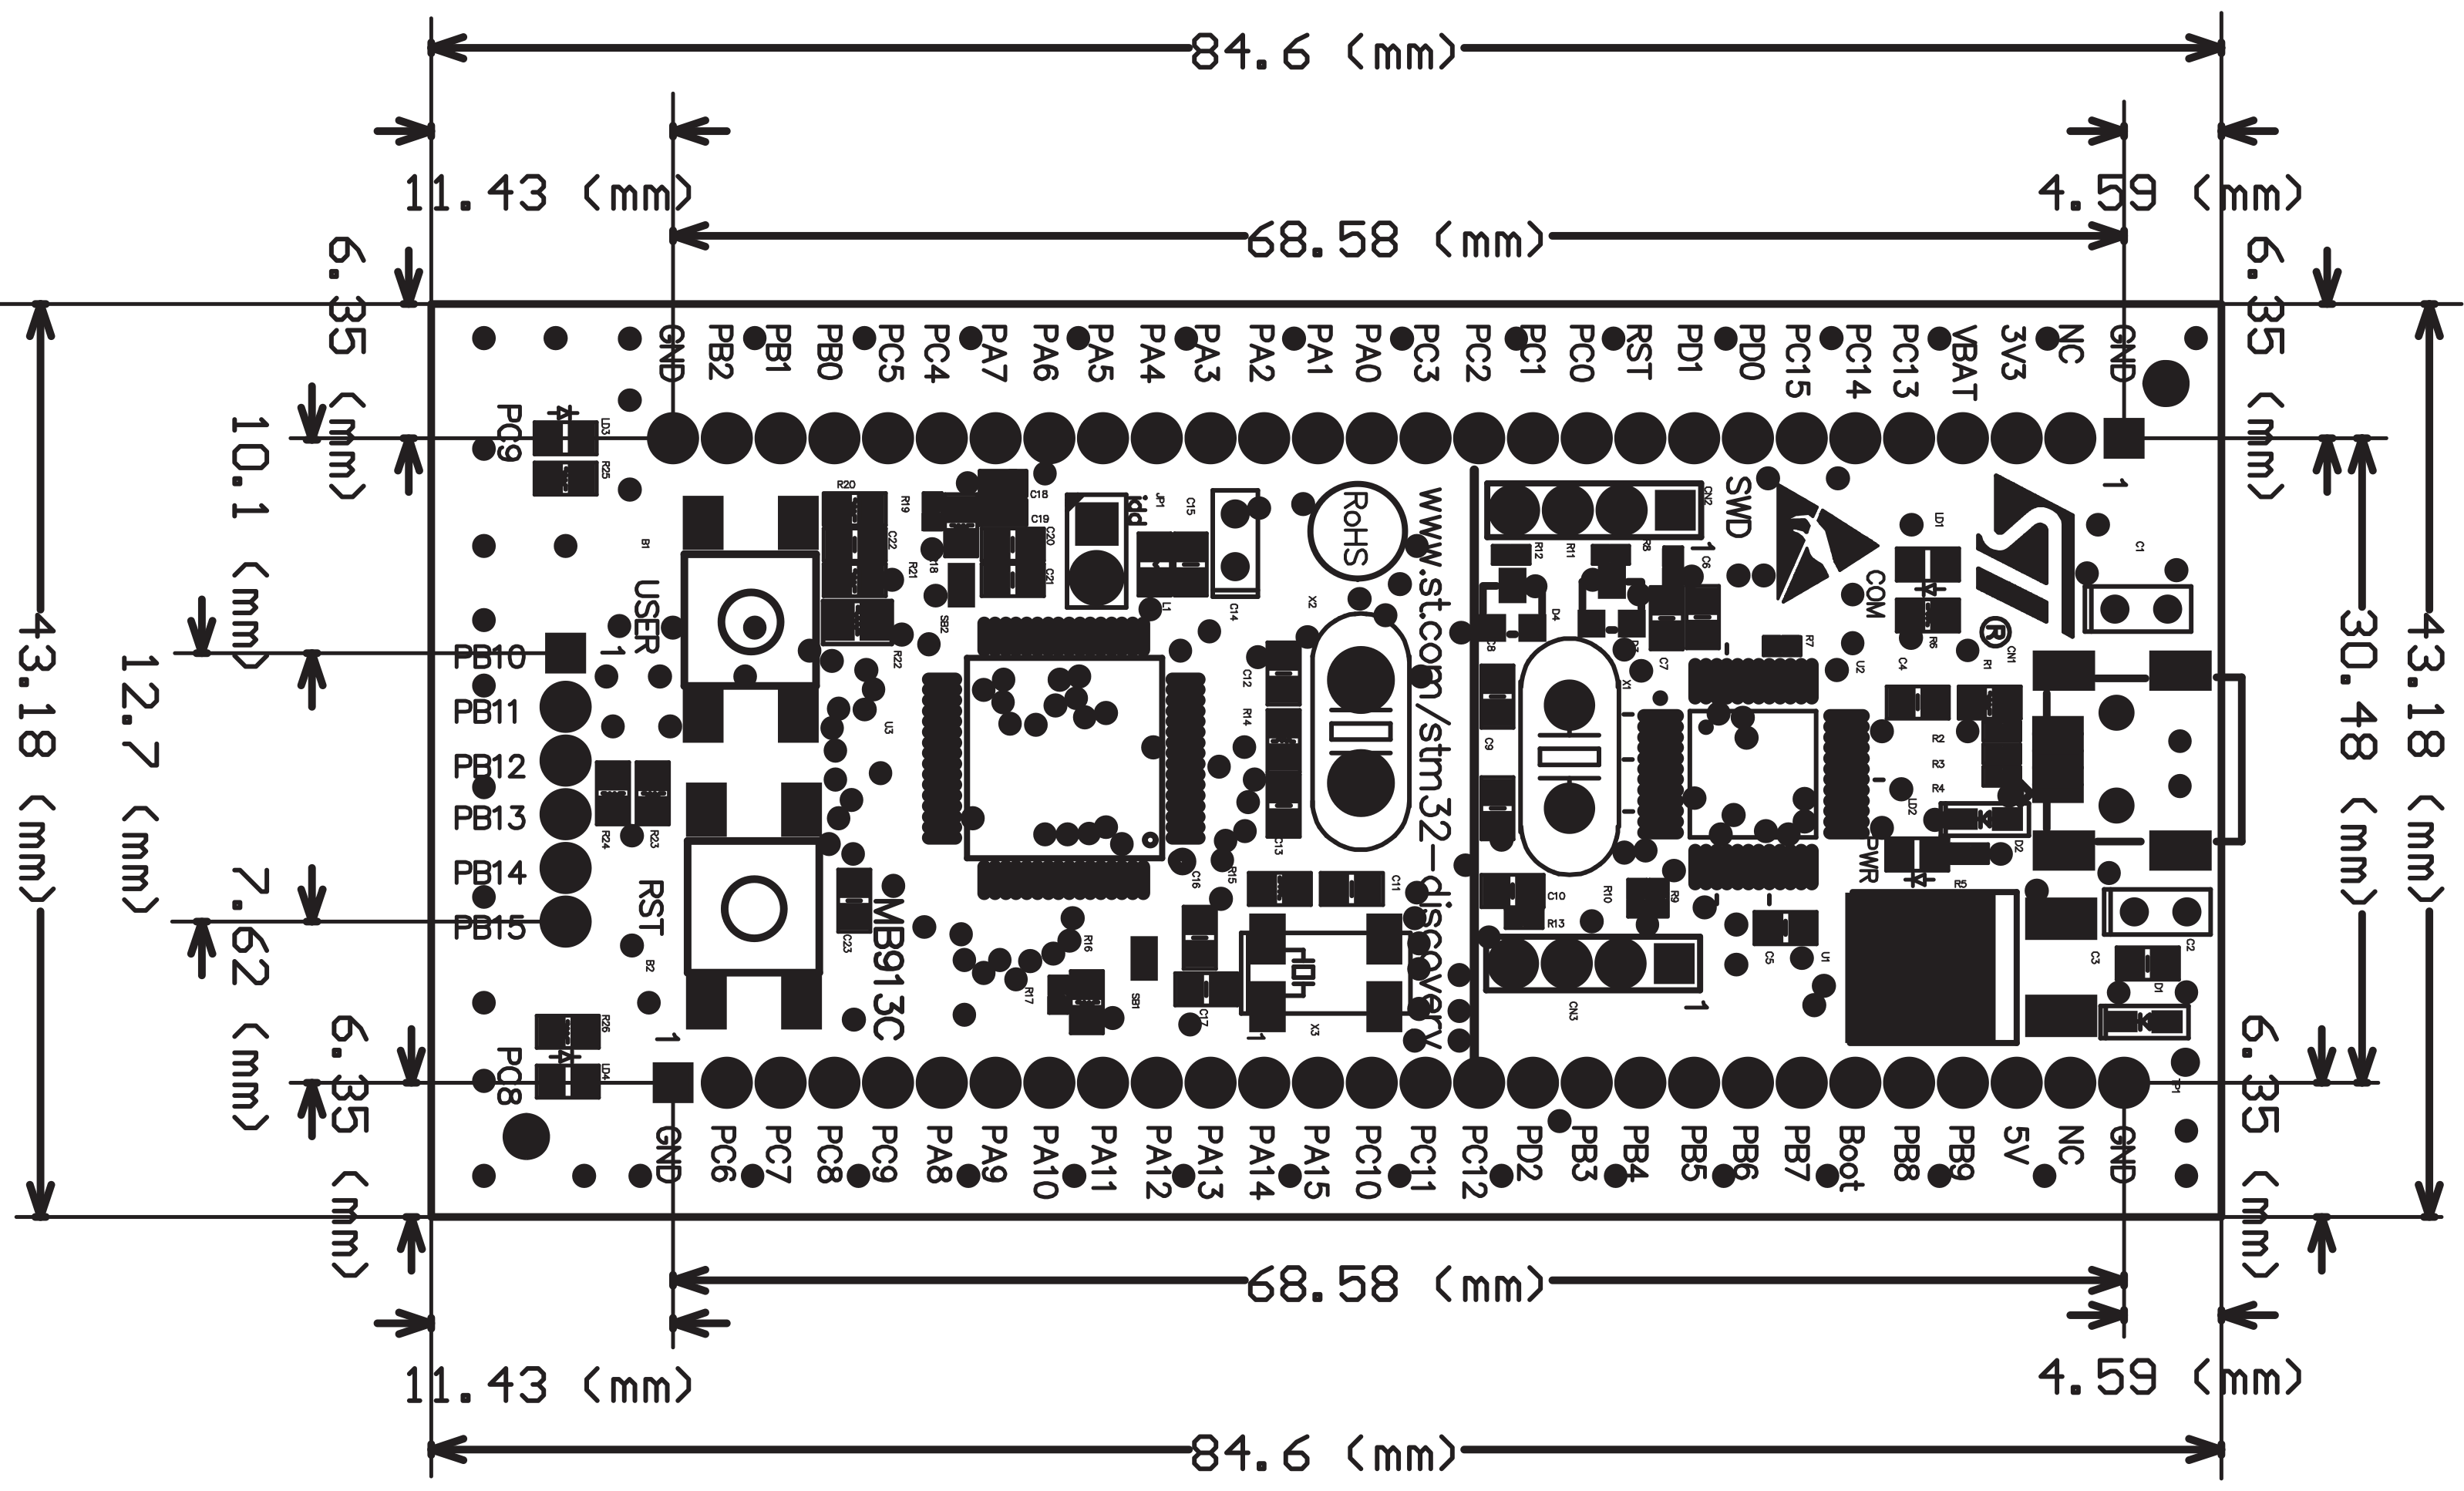
\includegraphics[width=0.8\linewidth]{img/stm32vldiscovery}}
            \caption{Размеры и расположение элементов модуля STM32VLDiscovery}
            \label{fig:stm32vldiscovery}
        \end{sidewaysfigure}       

    \subsubsection{Описание микроконтроллера STM32F100RBT6B}
        Особенности микроконтроллера STM32F100R:
        \begin{itemize}
            \item Вычислительное ядро Cortex-M3;
            \item Максимальная тактовая частота: 24 МГц;
            \item Напряжение питания 2,0 — 3,6 В;
            \item 128 кбайт NOR flash памяти с количеством циклов перезаписи 10000;
            \item 8 кбайт статической оперативной памяти;
            \item 7-канальный контроллер прямого доступа в память;
            \item 51 линия портов ввода-вывода общего назначения;
            \item 12-битный 16-канальный АЦП с временем преобразования 1,2 мкс;
            \item 12-битный ЦАП;
            \item 16-битный таймер с расширенными функциями;
            \item шесть 16-битных таймеров общего назначения;
            \item Восемь коммуникационных интерфейсов (I2C, USART, SPI).
        \end{itemize}

        \begin{sidewaysfigure}
            \center{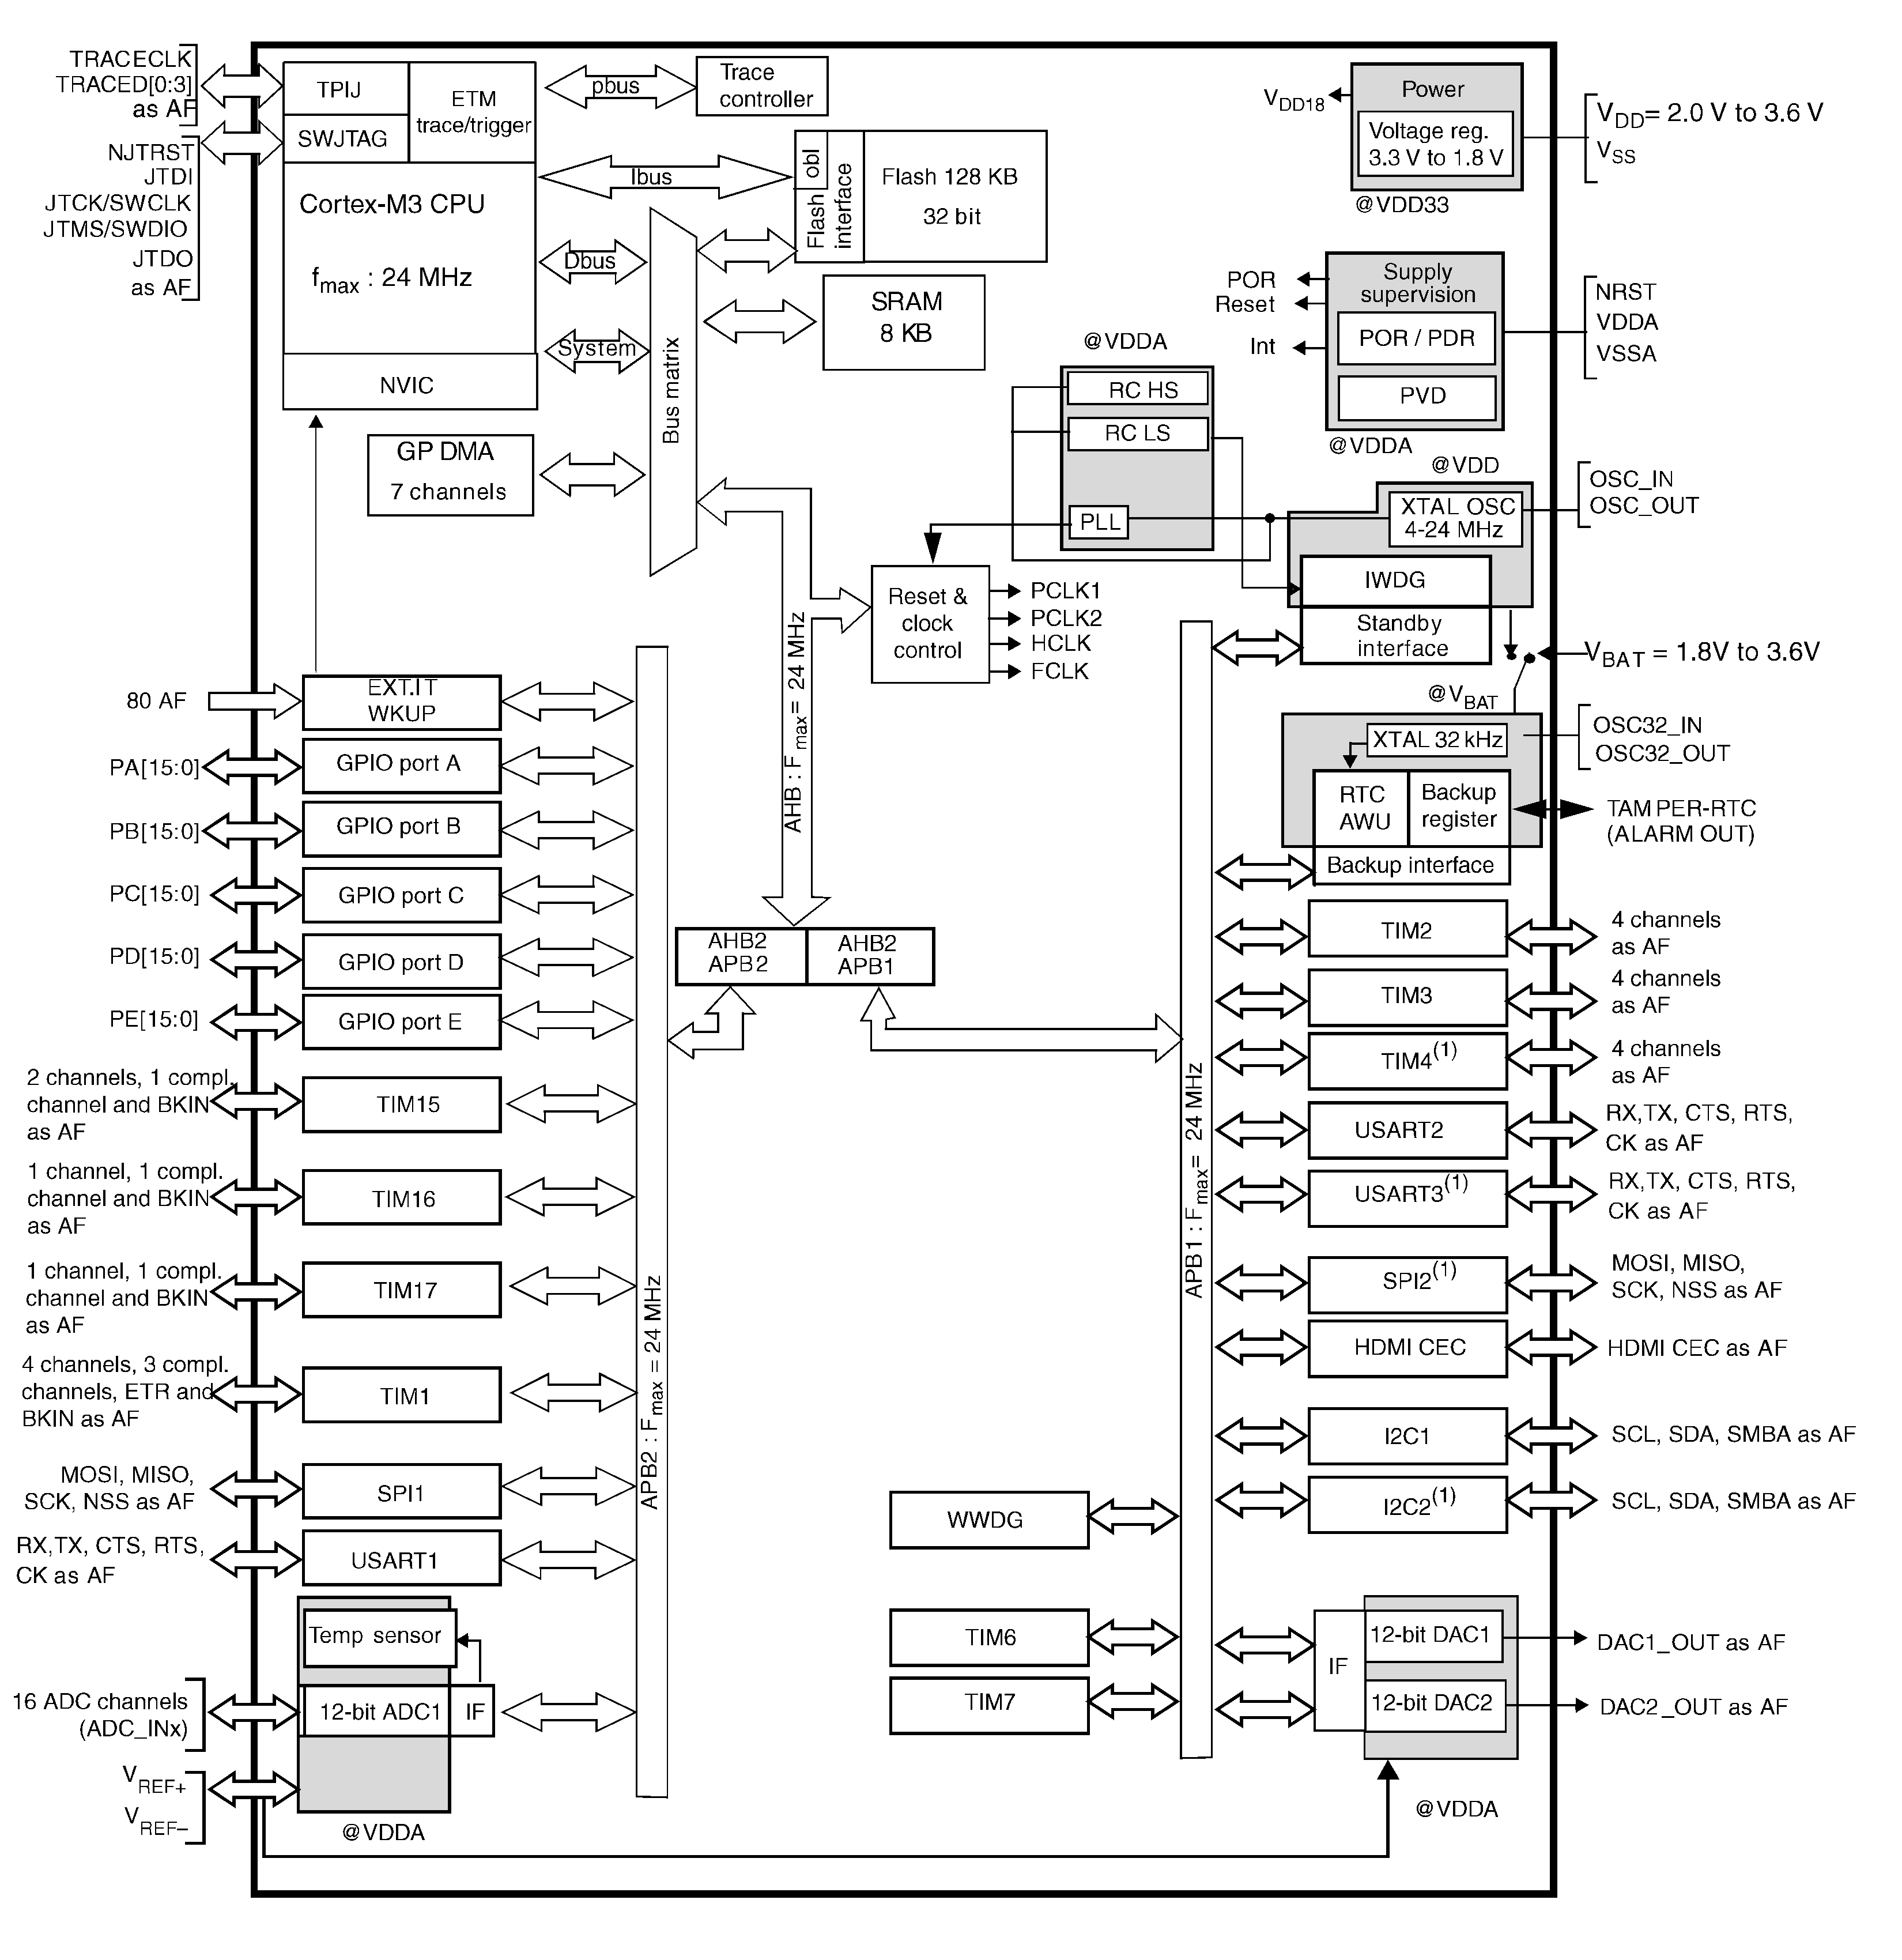
\includegraphics[width=0.65\linewidth]{img/stm32f100rbt6b}}
            \caption{Структурная схема микроконтроллера STM32F100RBT6B}
            \label{fig:stm32f100rbt6b}
        \end{sidewaysfigure}       
        
        Контроллер основан на высокопроизводительном 32 битном вычислительном
        ядре Cortex-M3 фирмы ARM.

        Cortex-M3 является стандартизованным микроконтроллерным ядром, которое
        помимо ЦПУ, содержит все остальные составляющие основу микроконтроллера
        элементы (в том числе приоритетный контроллер вложенных прерываний, 24
        битный системный таймер, интегрированный в ядро отладочный интерфейс). 

        4 гигабайтное адресное пространство Cortex-M3 разделено на четко
        распределенные области кода программы, статического ОЗУ, устройств
        ввода-вывода и системных ресурсов. Cortex-M3 выполнено по Гарвардской
        архитектуре и  имеет несколько шин, позволяющие параллельно выполнять
        такие операции как загрузка опкода, его выполнение (у МК имеется
        трехступенчатый конвеер), перемещение данных между регистрами и ОЗУ.

        Центральный процессорный элемент ядра Cortex-M3 имеет 13 регистров
        общего назначения, аппаратный 32 битный одноцикловый перемножитель,
        аппаратный делитель, а так же поддерживает два режима работы: потоковый
        режим (Thread) и режим обработчика (Handler), для каждого из которых
        можно сконфигурировать свои собственные стеки. Благодаря этому,
        появляется возможность разработки более интеллектуального программного
        обеспечения и поддержки операционных систем реального времени (ОСРВ) не
        только с кооперативной, но и с вытесняющей многозадачностью.

        Контроллер векторизированных вложенных прерываний (КВВП) может
        обрабатывать до 255 векторов, включая 15 исключений генерируемых
        процессорным ядром. КВВП также позволяет установить каждому вектору
        один из 16 уровней приоритета.

        Вход в процедуру обработки прерывания длится всего 12 машинных
        циклов, а на обработку каждого следующего вложенного прерывания
        процессор использует всего 6 циклов. Это достигнуто  за счет
        автоматического сохранения контекста прерванной программы и
        переключения стеков, выполняемых специальным микрокодом внутри ЦПУ.

        В ядро Cortex-M3 также входит 24-битный автоматически перезагружаемый
        таймер, предназначенный для генерации периодических прерываний и
        используемый ядром ОСРВ.

        Микроконтроллер имеет 16-битный таймер с возможностью управления
        трехфазным мостом силовых транзисторов. Таймер обеспечивает
        программируемое мертвое время, вход аварийной блокировки,
        настраиваемую полярность ШИМ сигнала.

        Два таймера общего назначения позволяют осуществлять обработку данных
        инкрементных энкодеров. Вычисление положения вала электродвигателя
        работает полнотью автоматически, независимо от ядра микроконтроллера.

        Семиканальный контроллер прямого доступа в память играет важную роль при
        программировании интерфейсов передачи данных, помогая существенно разгрузить
        вычислительное ядро.

        Хотя напряжение питания микроконтроллера 3,3В, практически все его
        порты ввода-вывода толерантны к напряжениям до 5В.

    \subsubsection{Описание цифровых изоляторов ADUM1300}
        ADuM1300 – трех канальные цифровые изоляторы компании Analog Devices.
        Отличительные особенности:
        \begin{itemize}
            \item низкое потребление (1.0 мА на канал на скорости до 10
                Мбит/с);
            \item двунаправленная передача данных;
            \item совместим с 3.3 В и 5.0 В питанием/уровнями логических
                сигналов;
            \item высокая скорость передачи данных: от 0 до 10 Мбит/с;
            \item максимальное искажение длительности импульса 2 нс;
            \item максимальное временное рассогласование каналов 2 нс;
            \item способность выдерживать воздействие изменяющегося входного
                синфазного сигнала, имеющего скорость нарастания более 25
                кВ/мкс;
            \item Функция активизации выходов;
            \item широкий 16 выводной SOIC корпус;
        \end{itemize}

        \begin{figure}[h!]
            \center{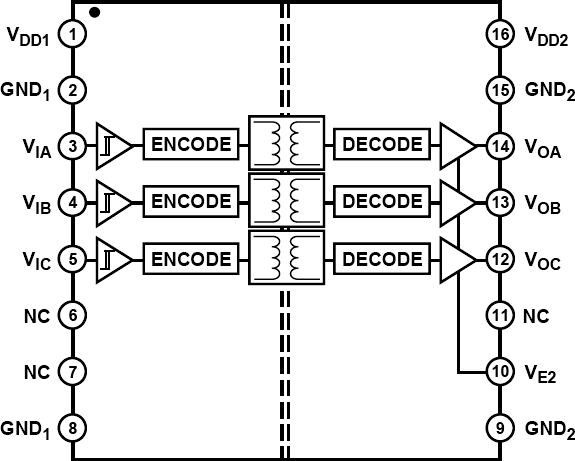
\includegraphics[width=0.8\linewidth]{img/adum1300}}
            \caption{Структурная схема цифрового изолятора ADUM1300}
            \label{fig:adum1300}
        \end{figure}

        Изоляторы семейства ADUM130X имеют три независимых канала и выпускаются
        в трех модификациях с различной пропускной способностью. Прибора
        ADuM1300 работает от однополярного источника питания, подключенного к
        любой стороне прибора, от 2,7 до 5,5 В, что позволяет обеспечить
        совместимость с низковольтными системами и произвести преобразование
        уровней сигналов через изоляционный канал. Кроме того, приборы ADUM130X
        обеспечивают низкие искажение ширины импульсов и временное
        рассогласование каналов.  Изоляторы ADUM130X имеют запатентованную
        функцию регенерации, которая гарантирует передачу статических
        параметром логических сигналов.

    \subsection{Разработка и реализация программной части системы управления АИН}
        Управляющее программное обеспечение электропривода
        лабораторно-исследовательского стенда полностью реализовано на языке C
        согласно стандарту С89. Компиляция осуществлялаь пакетом программ ARM
        GCC из набора GNU Compiler Collection. Автоматизация сборки реализована
        средствами GNU Make.

        Контроль версий производиться с помощью систмы Git. Репозиторий
        исходного кода расположен по адресу
        https://github.com/reviakinea/acid.git.

    \subsubsection{Программный синтез трехфазной системы синусоидальных напряжений}
        Под термином <<синтезатор частоты>> понимают электронное устройство,
        способное из опорной частоты получать на выходе требуемую частоту или
        набор частот,  согласно управляющим сигналам.

        DDS  уникальны своей цифровой определенностью:  генерируемый ими сигнал
        синтезируется со свойственной цифровым системам точностью.  Частота,
        амплитуда и фаза сигнала в любой момент времени точно известны и
        подконтрольны. DDS  практически не подвержены температурному дрейфу и
        старению.

        Основные преимущества DDS:  
        \begin{itemize}
            \item цифровое управление частотой и фазой выходного сигнала;
            \item очень высокое разрешение по частоте и фазе;
            \item экстремально быстрый переход на другую частоту (или фазу),
                перестройка по частоте без разрыва фазы,  без выбросов и других
                аномалий,  связанных с временем установления;
            \item архитектура,  основанная на DDS,  ввиду очень малого шага
                перестройки по частоте, исключает необходимость применения
                точной подстройки опорной частоты,  а также обеспечивает
                возможность параметрической температурной компенсации;
        \end{itemize}

        Частотное разрешение DDS  составляет сотые,  и даже тысячные доли герца
        при выходной частоте порядка десятков мегагерц.  Такое разрешение
        недостижимо для других методов синтеза. Другой характерной особенностью
        DDS  является очень высокая скорость перехода на другую частоту.  Более
        того,  все перестройки по частоте происходят у DDS  без разрыва фазы
        выходного сигнала.  Поскольку выходной сигнал синтезируется в цифровом
        виде,  очень просто осуществить модуляцию различных видов.

        Упрощенная блок-схема генератора прямого цифрового синтеза сигналов
        приведена на рисунке \ref{fig:dds-structure}. 

        \begin{figure}[h!]
            \center{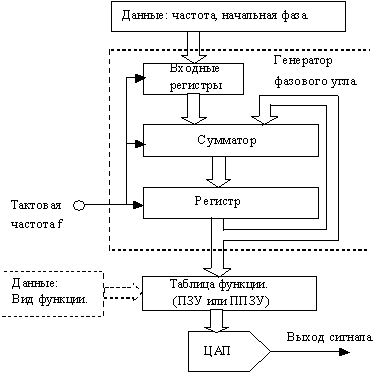
\includegraphics[width=0.55\linewidth]{img/dds-structure}}
            \caption{Структурная схема прямого цифрового синтеза частоты}
            \label{fig:dds-structure}
        \end{figure}

        Схема содержит три основных блока: генератор фазового угла, память и
        ЦАП. Генератор фазового угла в типичном случае представляет собой
        накапливающий сумматор с регистром. Работает он просто как регистр
        фазы, содержимое которого получает приращение на некоторый фазовый угол
        через заданные интервалы времени. Приращение фазы и её начальное
        значение загружаются в виде цифровых кодов во входные регистры. Память
        играет роль таблицы функций. Код текущей фазы поступает на ее адресные
        входы, а с выхода данных на вход цифроаналогового преобразователя
        поступает код, соответствующий текущему значению заданной функции.  ЦАП
        в свою очередь формирует аналоговый сигнал. В системе электропривода в
        роли ЦАП выступает генератор ШИМ сигнала и силовой блок АИН.

        Регистр содержит текущую фазу выходного сигнала в виде целого числа,
        которое при каждом тактовом импульсе получает приращение $\Delta n$,
        также целое число. Таким образом, текущий аргумент функции
        представляется целым числом Tn по модулю $2^N$, где $N$ -разрядность
        сумматора. Т.е.  последовательность значений аргумента является
        квазипериодической функцией. Дискретность по времени определяется
        тактовой частотой fc.  Увеличение разрядности регистра повышает
        разрешающую способность приращения аргумента $\Delta n$. Значения
        функции округляются в соответствии с разрядностью ЦАП.

        Так как производится синтез гармонического колебания, фазовый угол
        $\varphi$ равен: $\varphi = 2\pi \cdot T_n$. Тогда частота выходного
        сигнала $F$ равна произведению частоты тактов $F_{DDS}$ на относительное
        приращение целочисленного аргумента:
        \begin{gather*}
            F = \frac{\Delta n \cdot F_{DDS}}{2^N}.
        \end{gather*}

        Листинг функии синтеза трехфазной системы напряжений:
        \begin{verbatim}
        void sine_generation_task(void)
        {
            uint8_t  index;
            uint16_t pwm;

            /* phase increment */
            m_phase += m_delta;
         
            /* phase U duty cycle */
            index = (m_phase + PHASE_SHIFT_U) >> 8;
            pwm = (sine_table[index] * m_amplitude) >> 7;

            pwm_load_u(PWM_ZERO + pwm);

            /* phase V duty cycle */
            index = (m_phase + PHASE_SHIFT_V) >> 8;
            pwm = (sine_table[index] * m_amplitude) >> 7;

            pwm_load_v(PWM_ZERO + pwm);

            /* phase W duty cycle */
            index = (m_phase + PHASE_SHIFT_W) >> 8;
            pwm = (sine_table[index] * m_amplitude) >> 7;

            pwm_load_w(PWM_ZERO + pwm);
        }
        \end{verbatim}

        Блок-схема функции изображена на рисунке \ref{fig:bs-dds}

        \begin{figure}[h!]
            \center{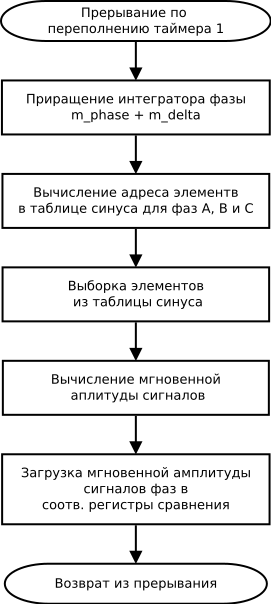
\includegraphics[width=0.40\linewidth]{img/bs-dds}}
            \caption{Блок-схема функции реализации цифрового синтеза трехфазной
                системы синусоидальных напряжений}
            \label{fig:bs-dds}
        \end{figure}

        В приведенном выше листинге роль накапливающего сумматора фазы играет
        16-битная переменная \verb"m_phase". На каждой итерации системы эта
        переменная получает приращение фазы $\Delta n$, которое храниться в
        \verb"m_delta". Аккумулятор фазы обеспечивает арифметику по модулю
        $2^{16}$, что соответствует переодичности функции синуса. 

        Далее, из таблицы значений функции синуса (индекс в таблице
        соответствует восьми старшим переменной \verb"m_phase") выбирается
        значение и перемножается на амплитуду. Эта последовательность
        повторяется для остальных двух фаз, за исключением сдвига фазы сигнала.

        На вход блока синтеза трехфазной системы синусоидальных напряжений
        поступают два сигнала: амплитуда сигнала $A$ (в переменной
        \verb"m_amplitude") и приращение фазы $\Delta n$ (в переменной
        \verb"m_delta"). Частота выходного сигна определяется по формуле:
        \begin{gather*}
            F = \frac{\Delta n \cdot F_{DDS}}{2^{16}},
        \end{gather*}

        где $F_c$ -- частота следования итераций алгоритма (в данном случае
        $F_{DDS} = 12$ КГц).

        Амплитуда выходного сигнала:
        \begin{gather*}
            A_\text{вых} = \frac{U_\text{п} \cdot A}{2000},
        \end{gather*}

        где $U_\text{п}$ -- выпрямленное напряжение питания инвертора. 

%        ШИМ сигнал управления трехфазным мостом АИН формируется блоком
%        сравнения таймера 1 микроконтроллера.
    \subsubsection{Релизация скалярного закона управления}
        Закон управления $V/f = const$ реализован в функции, листинг которой приведен ниже:
        \begin{verbatim}
            unsigned int vf_control(int frequency)
            {
                unsigned int amplitude;

                frequency = abs(frequency);

                /* Vf law */
                amplitude = frequency * VF_SLOPE / 256;

                /* Amplitude saturation */
                if (amplitude > VF_MAX_AMPLITUDE)
                {
                    amplitude = VF_MAX_AMPLITUDE;
                } 
                else if (amplitude < VF_MIN_AMPLITUDE)
                {
                    amplitude = VF_MIN_AMPLITUDE;
                }

                return amplitude;
            }
        \end{verbatim}
        
        Входным параметром данной функции является частота синусоидального
        сигнала. В соответствии со входным параметром и наклоном
        характеристики, заданным константой \verb"VF_SLOPE", функция возвращает
        необходимое напряжение питания статора электродвигателя. Выходное
        значение, также, ограничивается в пределах значения констант
        \verb"VF_MIN_AMPLITUDE" и \verb"VF_MAX_AMPLITUDE".
        Блок-схема функции изображена на рисунке \ref{fig:bs-vf}.

        \begin{figure}[ph!]
            \center{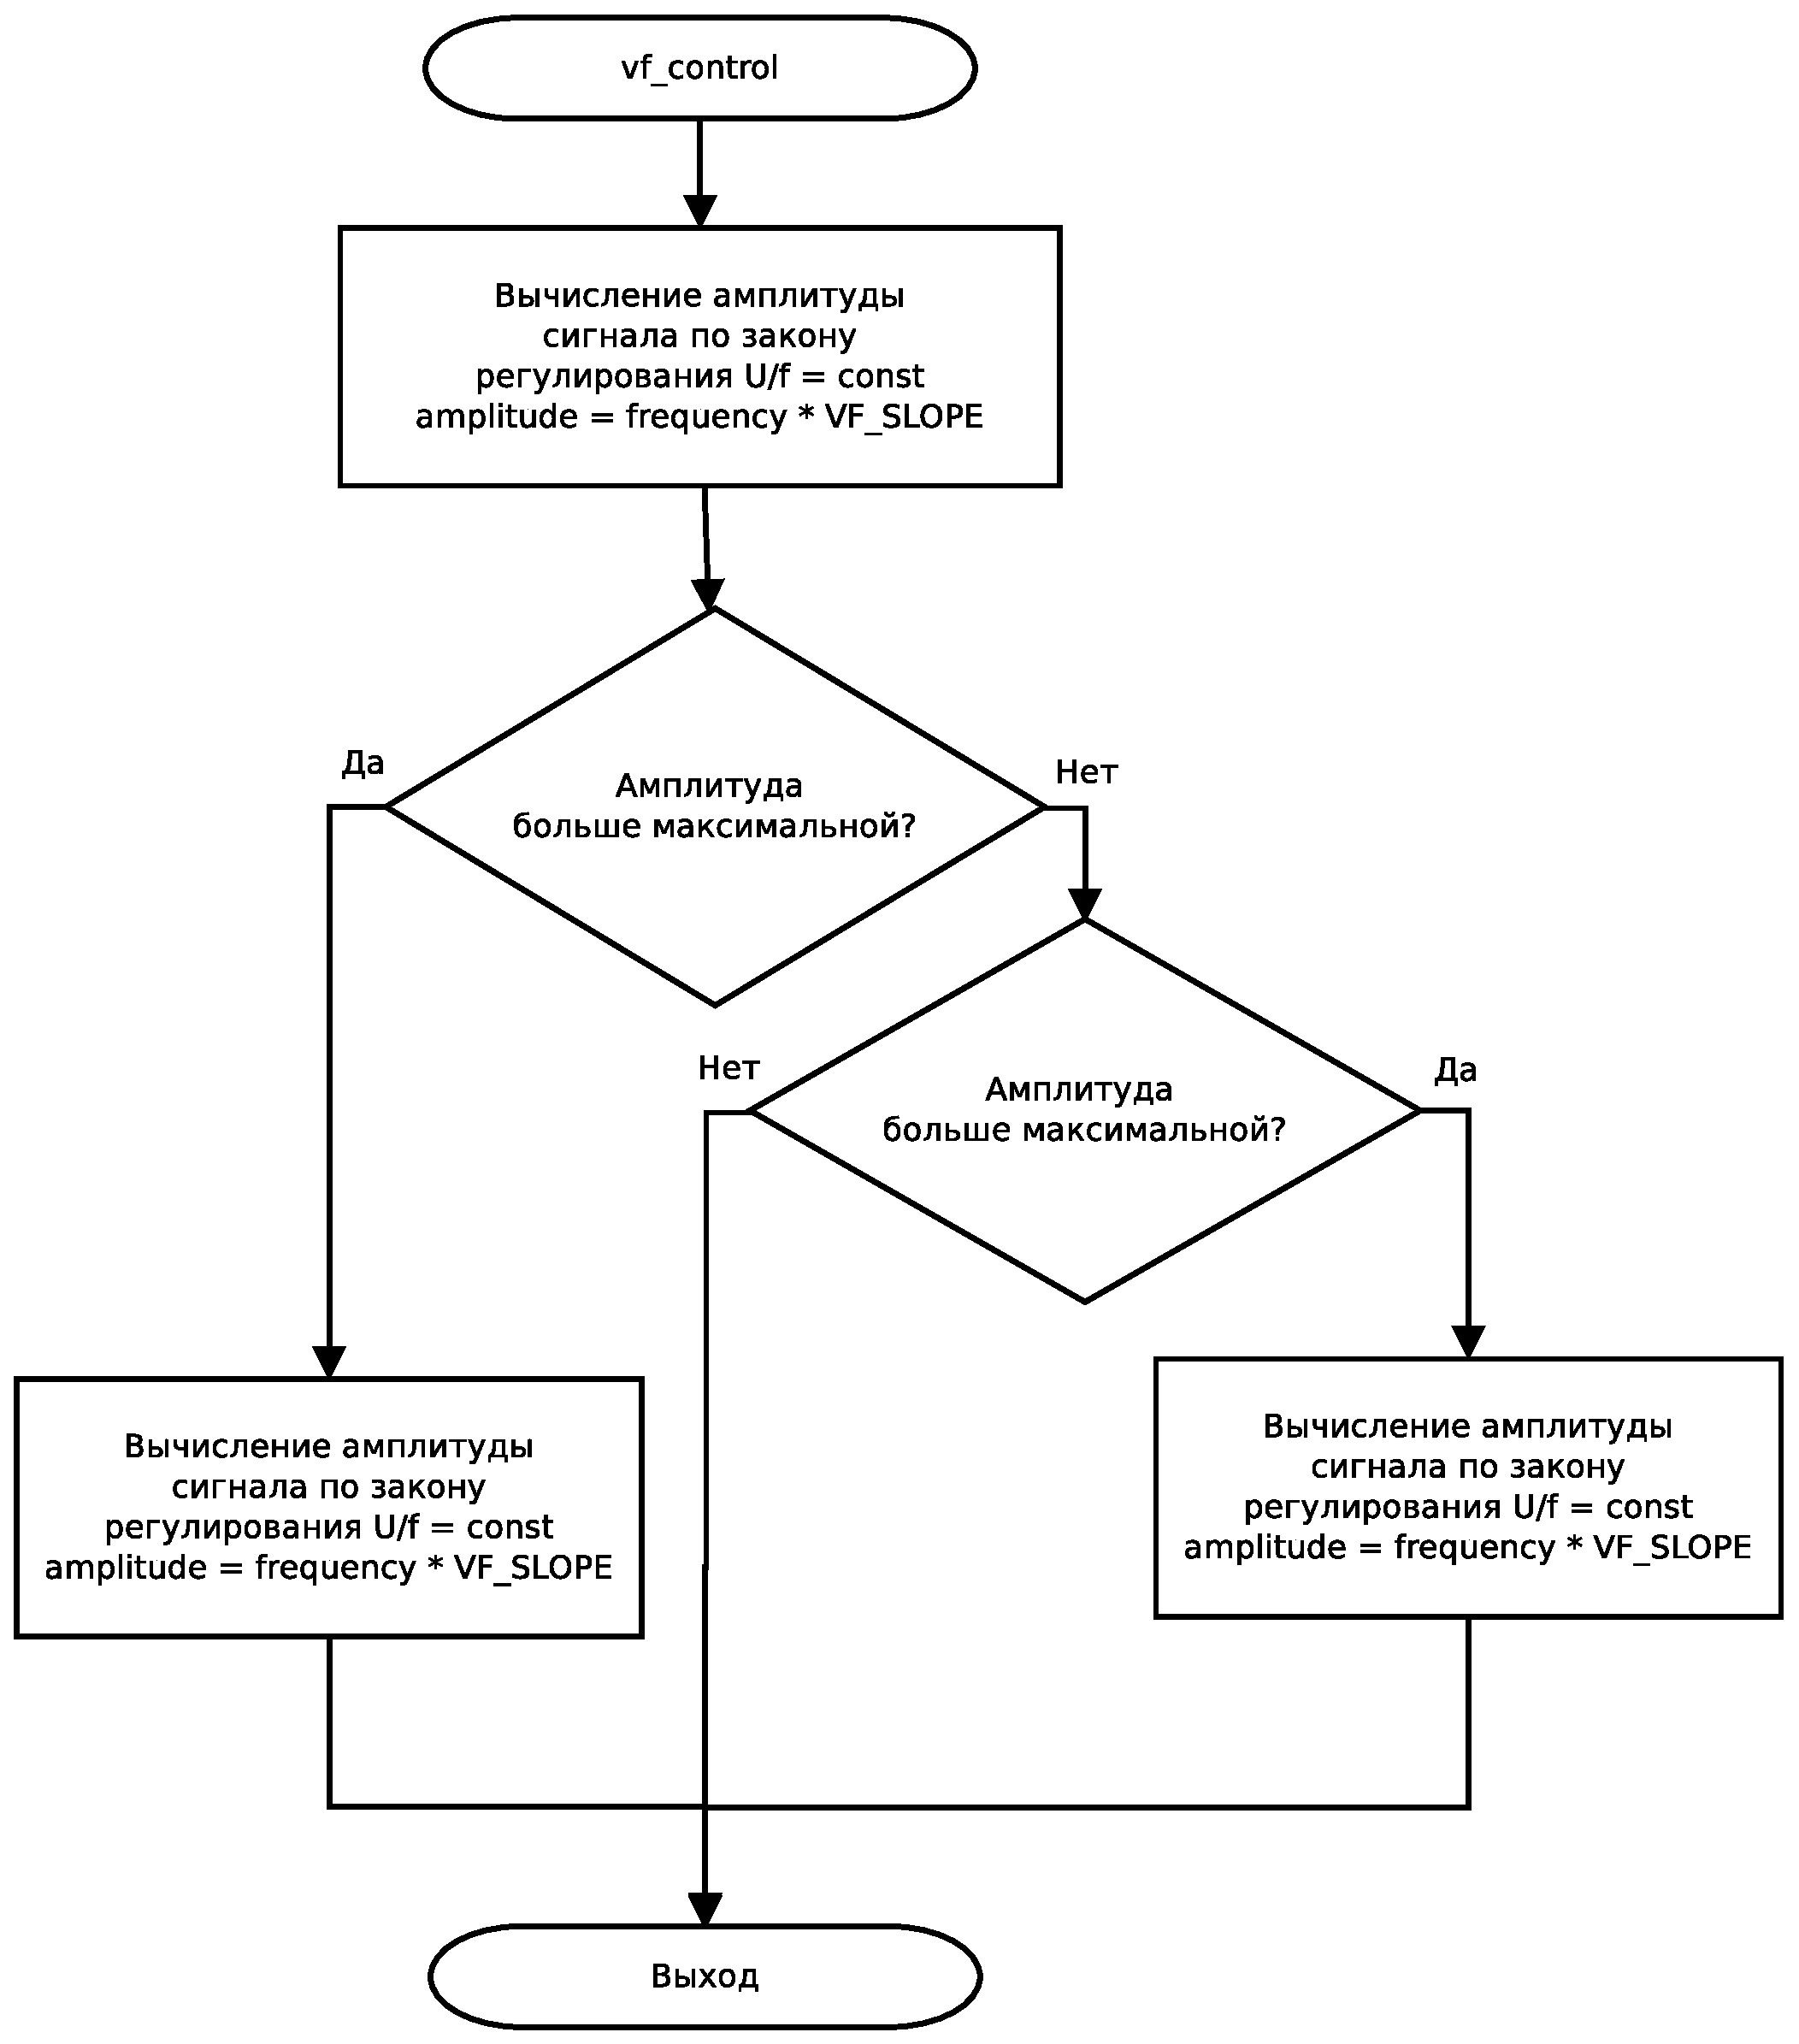
\includegraphics[width=1.0\linewidth]{img/bs-vf}}
            \caption{Блок-схема функции реализации постоянства соотношения $U/f$}
            \label{fig:bs-vf}
        \end{figure}
        
        Значение константы \verb"VF_SLOPE" определяется следующим отношением:
        \begin{gather*}
            V/f = \frac{U_\text{н}}{f_\text{н}} \cdot \frac{K_{DDS}}{2000} \cdot 256,
        \end{gather*}

        где $U_\text{н}$ -- номинальное напряжение питания электродвигателя;\par
        $f_\text{н}$ -- номинальная частота питающего напряжения электродвигателя;\par
        $K_{DDS}$ -- коэффициент передачи модуля синтеза частоты.

        Коэффициент передачи синтезатора определяется так:
        \begin{gather*}
            K_{DDS} = \frac{F_{DDS}}{2^{16}},
        \end{gather*}

        где $F_{DDS}$ -- частота приращения фазы синтезатора (в данном случае
        $F_{DDS} = 12$ КГц).

        Для данного двигателя наклон прямой зависимости напряжения питания от
        частоты выражается следующей формулой:
        \begin{gather*}
            V/f = \frac{220}{50} \cdot \frac{12000}{2^{16}} \cdot 256 = 206
        \end{gather*}

    \subsubsection{Реализация дискретного ПИД-регулятора}
        Для стабилизации скорости частоты вращения вала электродвигателя был
        применен дискретный ПИД-регулятор. Регулятор реализован программно
        внутри управляющего ПО системы электропривода.

        \begin{figure}[h!]
            \center{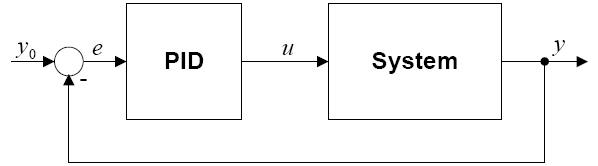
\includegraphics[width=0.8\linewidth]{img/system-with-pid}}
            \caption{Структурная схема системы с ПИД-регулятором}
            \label{fig:system-with-pid}
        \end{figure}

        На рисунке \ref{fig:system-with-pid} показана схема системы с
        ПИД-регулятором. На вход ПИД-регулятора поступает значение частоты
        вращения ротора электродвигателя, снятое с датчика скорости. Регулято
        сравнивает измеренное значение частоты вращения  с заданным опорным
        значением. Затем разница, или ошибка, E, обрабатывается для расчета
        сигнала задания. Этот сигнал задания будет пытаться приблизить значение
        измеряемого параметра (частоты вращения вала) к заданному значению.

        Альтернативой системе управления с замкнутым контуром, является система
        управления с открытым контуром. Применение открытого контура управления
        (без обратной связи) в данном случае не является удовлетворительным.

        В отличие от простых алгоритмов управления, ПИД-регулятор способен
        управлять процессом, основываясь на его истории и скорости изменения.
        Это дает более точный и стабильный метод управления.

        Структурная схема ПИД-регулятора показана на рисунке \ref{fig:pid}, где
        $T_p$, $T_i$, и $T_d$ обозначают постоянные времени пропорциональной,
        интегральной, и дифференциальной составляющих соответственно.

        Передаточная функция системы, изображенной на рисунке \ref{fig:pid}
        имеет вид:
        \begin{gather*}
            \frac{u}{e}(s) = H(s) = K_p \left(1 + \frac{1}{T_i s} + T_d s\right).
        \end{gather*}

        Отсюда имеем:
        \begin{gather*}
            u(t) = K_p \left( e(t)+\frac{1}{T_i} 
                \int \limits_0^t e(\sigma)d \sigma + T_d \frac{de(t)}{dt} \right).
        \end{gather*}

        Пропорциональная составляющая (П) дает управляющий сигнал
        пропорционально вычисленной ошибке. Использование только одного
        пропорционального управления дает стационарную ошибку всегда, кроме
        случаев, когда управляющий сигнал равен нулю, а значение системного
        процесса равно требуемой величине.Использование слишком большого
        П-члена даст неустойчивую систему. 

        Интегральная составляющая (И) представляет собой предыдущих ошибок.
        Суммирование ошибки будет продолжаться до тех пор, пока значение
        системного процесса не станет равно нужному значению. Обычно
        интегральную составляющую используют вместе с пропорциональной, в так
        называемых ПИ-регуляторах. Использование только интегральной
        составляющей дает медленный отклик и часто колебательную систему.
        Отклик ПИ-регулятора не имеет стационарной ошибки, а отклик
        И-регулятора очень медленной.

        Дифференциальная составляющая (Д) представляет собой скорость изменения
        ошибки. Добавление этой составляющей улучшает отклик системы на
        внезапное изменение ее состояния. Дифференциальная составляющая Д
        обычно используется с П или ПИ алгоритмами, как ПД или ПИД контроллеры.
        Большая дифференциальная составляющая Д обычно дает неустойчивую
        систему. Отклик ПД-контроллера дает быстрый рост значения процесса, чем
        П контроллер. Обратите внимание, что дифференциальная составляющая Д
        ведет себя по существу как фильтр верхних частот для сигнала ошибки и,
        таким образом легко делает систему нестабильной и более чувствительной
        к шуму.

        Аппроксимируем интегральную и дифференциальную составляющие, чтобы
        получить дискретный вид:
        \begin{gather*}
            \int \limits_0^t e(\sigma)d\sigma \approx T \sum \limits_{k=0}^n e(k),\\
            \frac{de(t)}{dt} \approx \frac{e(n) - e(n - 1)}{T},\\
            t = nT,
        \end{gather*}

        где $n$ -- дискретный шаг времени t.

        Это дает нам такой регулятор:
        \begin{gather*}
            u(n) = K_p e(n) + K_i \sum \limits_{k=0}^n e(k) + K_d (e(n)-e(n-1));
        \end{gather*}

        Где
        \begin{gather*}
            K_i = \frac{K_p T}{T_i};\\
            K_d = \frac{K_p T_d}{T}.
        \end{gather*}

        Реализация ПИД-контоллера на языке С представлена ниже:
        \begin{verbatim}
            #define SCAL_FACTOR 1024
            #define P_TERM_MAX  (INT32_MAX / 4)
            #define I_TERM_MAX  (INT32_MAX / 4)

            typedef struct {

                /* PID koeff. */
                uint16_t    p_factor;
                uint16_t    i_factor;
                uint16_t    d_factor;

                /* Int. term summator */
                int32_t     sum_error;

                /* Last measured value. Use for diff. term */
                int16_t     last_meas;

                /* Max values */
                int32_t     max_sum;
                int32_t     max_error;
            } pidc_t;
            void pid_init( pidc_t *pid, uint16_t p_factor,
                uint16_t i_factor, uint16_t d_factor )
            {
                /* Reset PID */
                pid->last_meas = 0;
                pid->sum_error = 0;

                /* Tuning */
                pid->p_factor = p_factor;
                pid->i_factor = i_factor;
                pid->d_factor = d_factor;

                /* Calculate max values */
                pid->max_error = P_TERM_MAX / (pid->p_factor + 1);
                pid->max_sum   = I_TERM_MAX / (pid->i_factor + 1);
            }
            int16_t pid_controller( pidc_t *pid, 
                int16_t ref, int16_t meas )
            {
                int32_t p_term, i_term, d_term;
                int32_t error, temp;

                error = ref - meas;

                if ( error > pid->max_error ) {
                    p_term = P_TERM_MAX;
                } else if ( error < -pid->max_error ) {
                    p_term = -P_TERM_MAX;
                } else {
                    p_term = pid->p_factor * error;
                }

                temp = pid->sum_error + error;
                if ( temp > pid->max_sum ) {
                    i_term = I_TERM_MAX;
                } else if ( temp < -I_TERM_MAX ) {
                    i_term = -I_TERM_MAX;
                } else {
                    pid->sum_error = temp;
                    i_term = pid->i_factor * pid->sum_error;
                }

                d_term = pid->d_factor * pid->last_meas - meas;
                pid->last_meas = meas;

                return (int16_t) ((p_term + i_term + d_term) 
                    / SCAL_FACTOR);
            }
        \end{verbatim}

        Все данные ПИД-регулятора хранятся в структуре \verb"pidс_t". Функция\\
        \verb"pid_init()" получает на вход коэффициенты регулятора и
        инициализирует структуру ПИД. Функция \verb"pid_controller()" вычисляет
        сигнал управляющего воздействия по переданным ей значениям сигнала
        задания и измереного значения частоты вращения.

        Блок-схема функции ПИД-регулятора изображена на рисунке \ref{fig:bs-pid}.

        \begin{figure}[ph!]
            \center{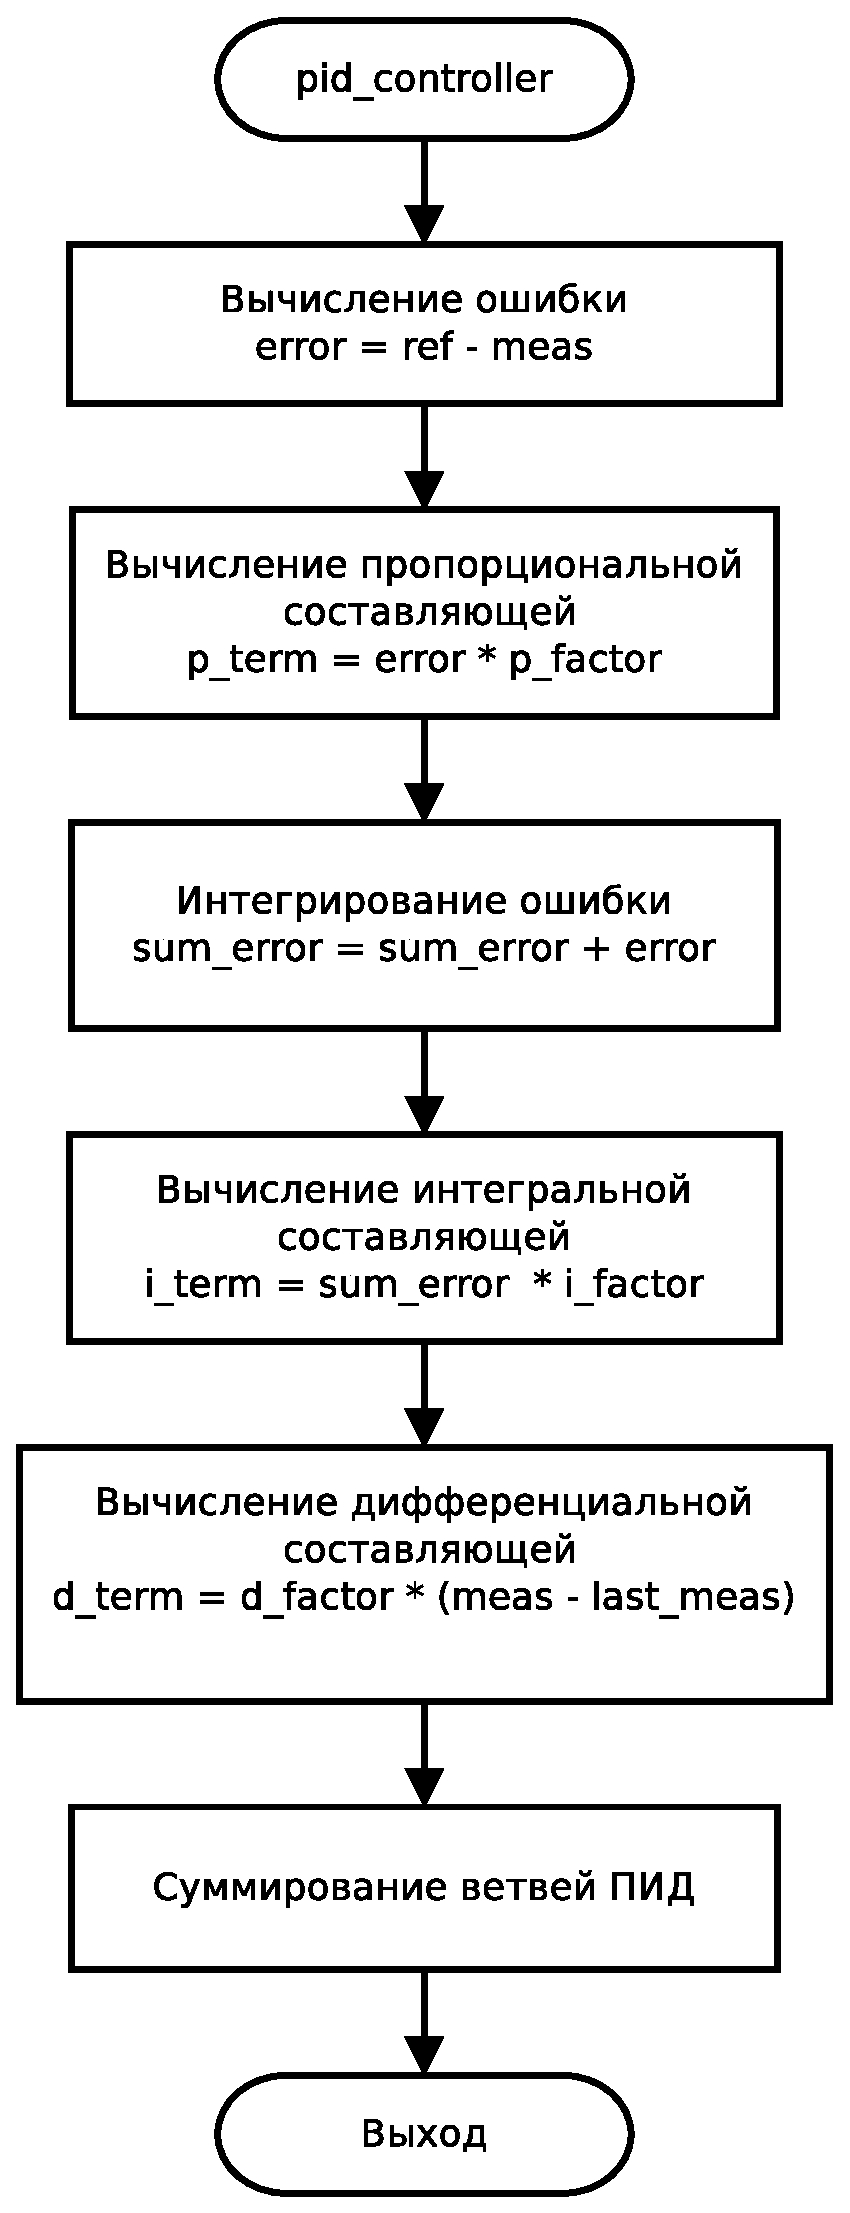
\includegraphics[width=0.45\linewidth]{img/bs-pid}}
            \caption{Блок-схема функции реализации дискретного ПИД-регулятора}
            \label{fig:bs-pid}
        \end{figure}

    \newpage
    \subsubsection{Реализация протокола передачи данных Modbus RTU}
        Для взаимодействия с управляющим персональным копьютером в программное
        обеспечение системы управления был добавлен алгориитм, реализующий
        стандартизированный бинарный протокол передачи данных Modbus RTU. Выбор
        протокола передачи данных основан на простоте реализации и многообразии
        уже написанного ПО для отладки и обмена данными по этому протоколу.

        Modbus — открытый коммуникационный протокол, основанный на архитектуре
        <<клиент-сервер>>. Широко применяется в промышленности для организации
        связи между электронными устройствами. Может использоваться для
        передачи данных через последовательные линии связи RS-485, RS-422,
        RS-232, а также сети TCP/IP (Modbus TCP).

        Контроллеры на шине Modbus взаимодействуют, используя клиент-серверную
        модель, основанную на транзакциях, состоящих из запроса и ответа.

        Обычно в сети есть только один клиент, так называемое, <<главное>> 
        (master) устройство, и несколько серверов — <<подчиненных>> (slaves)
        устройств. Главное устройство инициирует транзакции (передаёт запросы).
        Главный может адресоваться индивидуально к подчиненному или
        инициировать передачу широковещательного сообщения для всех подчиненных
        устройств. Подчиненное устройство отвечает на запрос, адресованный
        именно ему. При получении широковещательного запроса ответ не
        формируется.

        Спецификация Modbus описывает структуру запросов и ответов. Их основа —
        элементарный пакет протокола, так называемый PDU (Protocol Data Unit).
        Структура PDU не зависит от типа линии связи и включает в себя код
        функции и поле данных. Код функции кодируется однобайтовым полем и
        может принимать значения в диапазоне 1..127. Диапазон значений 128..255
        зарезервирован для кодов ошибок. Поле данных может быть переменной
        длины. Размер пакета PDU ограничен 253 байтами.

        Для передачи пакета по физическим линиям связи PDU помещается в другой
        пакет, содержащий дополнительные поля. Этот пакет носит название ADU
        (Application Data Unit).Общая структура ADU следующая:
        
        \begin{itemize}
            \item адрес ведомого устройства — адрес подчинённого устройства, к
                которому адресован запрос. Ведомые устройства отвечают только
                на запросы, поступившие в их адрес. Ответ также начинается с
                адреса отвечающего ведомого устройства, который может
                изменяться от 1 до 247. Адрес 0 используется для
                широковещательной передачи, его распознаёт каждое устройство,
                адреса в диапазоне 248..255 — зарезервированы; 
            \item код функции — это следующее однобайтное поле кадра. Оно
                говорит ведомому устройству, какие данные или выполнение какого
                действия требует от него ведущее устройство; 
            \item данные — поле содержит информацию, необходимую ведомому
                устройству для выполнения заданной мастером функции или
                содержит данные, передаваемые ведомым устройством в ответ на
                запрос ведущего.  Длина и формат поля зависит от номера
                функции;
            \item блок обнаружения ошибок — контрольная сумма для проверки
                отсутствия ошибок в кадре.
        \end{itemize}

        Максимальный размер ADU для последовательных сетей RS232/RS485 — 256
        байт, для сетей TCP — 260 байт. 

        Ошибки передачи данных обнаруживаются при помощи фреймов символов,
        контроля чётности и циклической контрольной суммы CRC-16-IBM
        (используется число-полином = 0xA001). 

        Наличее в микроконтроллере контроллера прямого доступа в память
        позволило реализовать очень быстрый и нетребовательный к ресурсам
        алгоритм обмена данными. Что позволило поднять скорость передачи данных
        до 480 Кбит/с.

    \subsection{Моделирование системы скалярного управления асинхронного
        электропривода с к. з. ротором}

        Асинхронный привод со скалярным частотным управлением используется для
        механизмов средней и малой мощности, который не требуют глубокого
        регулирования скорости и высокого качества переходных процессов.

        Уравнение электромагнитных контуров АД в установившемся режиме будет
        иметь вид
        \begin{gather*}
            \left\{
            \begin{aligned}
                \frac{\tilde U_s}{\omega_s} =\tilde I_s\frac{Rs}{\omega_s}+
                    j\tilde \Psi_s=\tilde I_s\frac{R_s}{\omega_s}+
                        jL_{s\sigma}\tilde I_s +j\tilde \Psi_m\\
                0 = \tilde I_r\frac{R_r}{\beta}+j\tilde \Psi_r =
                    \tilde I_r\frac{R_r}{\beta}+jL_{r\sigma}\tilde I_r+
                        j \tilde \Psi_m,\\
            \end{aligned}
            \right.
        \end{gather*}

        где $\beta = \omega_s - \omega_r = S\omega_s$ -- абсолютное скольжение АД;\par
        $\tilde \Psi_m = L_m \tilde I_m = L_m(\tilde I_s + \tilde I_r)$ -- потокосцепление
        в воздушном зазоре.

        Приведенной системе уравнений соответствует эквивалентная схема
        замещения, которая представлена на рисунке \ref{fig:ad-zam}.  

        \begin{figure}[h!]
            \center{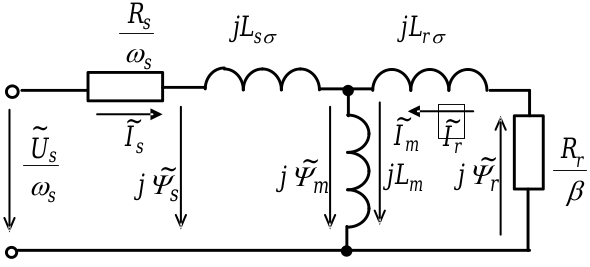
\includegraphics[width=0.6\linewidth]{img/ad-zam}}
            \caption{Эквивалентная схема замещения асинхронного двигателя с к. з. ротором}
            \label{fig:ad-zam}
        \end{figure}

        Передаточная функция регулятора напряжения внешнего контура в виде
        \begin{gather*}
            W_{PUs}(p)=\frac{\pi}{2\sqrt{3}}\cdot\frac{k_{Id}}{k_{Us}R_D} \cdot
                \frac{(T_D + T_F) p+1}{T_{H2}p},
        \end{gather*}

        где $k_v$ -- коэффициент усиления КВ.

        \begin{gather*}
            R_D = \frac{\pi^2}{18} \cdot \frac{L_s}{T_r(1 - \sigma)S_1},
        \end{gather*}

        где $T_D=R_D C_F$ -- эквивалентное сопротивление и эквивалентная
        постоянная времени объекта <<АИН -- АД>>;\par
        $S_1$ -- расчетный параметр,
        который косвенно отображает желаемую жесткость механических
        характеристик ЭП (для расчетов можно принять равным 0,1);\par
        $k_{Ui}$ -- коэффициент передачи датчика напряжения на входе АИН; 
        $T_H = k_{kUi}Tv$ --квивалентная постоянная времени интегрирования
            регулятора напряжения на входе АИН;\par
        $k_{kUi}$ -- аладочный коэффициент, значения которого превышают 1. 

        С помощью ПЧ может быть реализована нужная зависимость напряжения
        статора АД от частоты. Закон частотного регулирования, который
        реализованный в ПЧ должен выполняться при $U_S \leq U_{SH}$ для
        предотвращения питания АД увеличенным напряжением. При необходимости
        дальнейшего повышения частоты вращения напряжение статора АД должно
        быть ограничено, а регулирование скорости в этой зоне осуществляется
        лишь за счет повышения частоты.

    \subsection{Математическое описание и динамическая модель АД как обобщенной
        электрической машины}

        Структурная схема модели в фазных координатах получается весьма сложной
        из-за наличия переменных коэффициентов в уравнениях связи фазных токов
        и потокосцеплений машины, зависящих от мгновенного значения угла
        поворота ротора относительно магнитных осей статора двигателя. С целью
        упрощения математических моделей систему уравнений трехфазной
        асинхронной машины, записанную в фазных координатах, принято
        представлять в ортогональной системе координат (х–у), вращающейся в
        пространстве в общем случае с произвольной угловой скоростью $\omega_k$.

        Эквивалентные напряжения статора в системе координат (х–у) связаны с
        фазными напряжения трехфазной машины следующими соотношениями
        \begin{gather*}
            U_{sx} = \frac{2}{3} \left[ U_\text{ФА}\cos\omega_k t+U_\text{ФВ}
                \cos\left(\omega_k t-\frac{2\pi}{3}\right)+U_\text{ФС} \cos
                    \left( \omega_k t+\frac{2\pi}{3}\right)\right],\\
            U_{sy} = -\frac{2}{3} \left[ U_\text{ФА}\cos\omega_k t+U_\text{ФВ}
                \cos\left(\omega_k t-\frac{2\pi}{3}\right)+U_\text{ФС} \cos
                    \left( \omega_k t+\frac{2\pi}{3}\right)\right].\\
        \end{gather*}

        Аналогичные соотношения связывают эквивалентные значения токов и
        потокосцеплений двигателя с соответствующими фазными значениями
        переменных. Подставляя в эти уравнения выражения для реальных фазных
        напряжений
        \begin{gather*}
            U_\text{ФА} = U_m\cos(\omega_0 t + \varphi_0),\\
            U_\text{ФВ} = U_m\cos\left(\omega_0t-\frac{2\pi}{3}+\varphi_0\right),\\
            U_\text{ФC} = U_m\cos\left(\omega_0t+\frac{2\pi}{3}+\varphi_0\right),\\
        \end{gather*}

        Можно получить выражения для составляющих напряжений в эквивалентной
        2-хфазной системе координат
        \begin{gather*}
            U_{sx} = U_m \cos [(\omega_0 - \omega_k)t + \varphi_0],\\
            U_{sy} = U_m \sin [(\omega_0 - \omega_k)t + \varphi_0],\\
        \end{gather*}

        где $U_m$ -- амплитудное значение фазного напряжения;
        $\omega_0$ -- частота вращения поля статора двигателя в пространстве;
        $\varphi_0$ -- начальная фаза напряжения фазы А.

        Система уравнений электромагнитного равновесия асинхронного двигателя в
        форме Коши в системе координат (х–у) может быть представлена следующим
        образом
        \begin{gather*}
            \left\{
            \begin{aligned}
                \frac{d\Phi_{sx}}{dt} & = U_{sx} - R_s i_{sx} + \omega_k \Psi_{sy}\\
                \frac{d\Phi_{sy}}{dt} & = U_{sy} - R_s i_{sy} + \omega_k \Psi_{sx}\\
                \frac{d\Phi_{rx}}{dt} & = R_s i_{sx} + (\omega_k-\omega) \Psi_{ry}\\
                \frac{d\Phi_{ry}}{dt} & = R_s i_{sy} + (\omega_k-\omega) \Psi_{rx},\\
            \end{aligned}
            \right.
        \end{gather*}

        где $\Psi_{sx}, \Psi_{sy}$ -- потокосцепления эквивалентных статорных
            контуров;\par
        $\Psi_{rx}, \Psi_{ry}$ -- потокосцепления эквивалентных роторных
            контуров;\par
        $i_{sx}, i_{sy}$ -- эквивалентные  токи статора;\par
        $i_{rx}, i_{ry}$ -- эквивалентные  токи ротора;\par
        $R_s, R_r$ -- активные сопротивления фазных обмоток статора и ротора.

        Для решения этой системы уравнений ее необходимо дополнить уравнениями
        связи эквивалентных токов и потокосцеплений машины. В системе координат
        (х–у) эквивалентные потокосцепления и токи статора и ротора двигателя
        связаны друг с другом следующими уравнениями
        \begin{gather*}
            \left\{
            \begin{aligned}
                \Psi_{sx} & = L_s i_{sx} + L_m i_{rx}\\
                \Psi_{sy} & = L_s i_{sy} + L_m i_{rx}\\
                \Psi_{rx} & = L_s i_{sx} + L_r i_{rx}\\
                \Psi_{ry} & = L_s i_{sy} + L_r i_{rx}\\
            \end{aligned}
            \right.
        \end{gather*}
        
        где $L_m$ -- взаимная индуктивность, учитывающая магнитную связь одной
        фазы статора с тремя обмотками  ротора  и  соответственно  одной
        обмотки  ротора с тремя обмотками статора;

        $L_s=L_m+L_{\sigma s}$ -- индуктивность обмотки статора,
        учитывающая магнитную связь с двумя другими фазными обмотками
        статора;
        
        $L_r=L_m+L_{\sigma}$ -- индуктивность обмотки ротора, учитывающая
        магнитную связь с двумя другими фазными обмотками ротора;

        $L_{\sigma s}$ -- индуктивность рассеяния фазной обмотки статора;

        $L_{\sigma r}$ -- индуктивность рассеяния фазной обмотки ротора.

        Коэффициенты в уравнениях связи между эквивалентными токами и
        потокосцеплениями не зависят от мгновенного значения угла поворота
        ротора относительно магнитной оси статора двигателя. Для построения
        математической модели асинхронного двигателя удобнее пользоваться
        обратными зависимостями, то есть зависимостями $i=f(\Psi)$, которые
        имеют вид
        \begin{gather*}
            \left\{
            \begin{aligned}
                i_{sx} & =\frac{1}{\sigma L_s}\Psi_{sx}-
                    \frac{L_m}{\sigma L_s L_r}\Psi_{rx}\\
                i_{sy} & =\frac{1}{\sigma L_s}\Psi_{sy}-
                    \frac{L_m}{\sigma L_s L_r}\Psi_{ry}\\
                i_{rx} & =-\frac{L_m}{\sigma L_s}\Psi_{sx}+
                    \frac{1}{\sigma L_r}\Psi_{rx}\\
                i_{ry} & =-\frac{L_m}{\sigma L_s}\Psi_{sy}+
                    \frac{1}{\sigma L_r}\Psi_{ry},\\
            \end{aligned}
            \right.
        \end{gather*}

        где $\sigma=\left(1-\cfrac{L_m^2}{L_s L_r}\right)$ -- коэффициент
        рассеяния двигателя.

        Выражение для электромагнитного момента асинхронного двигателя
        представляет собой векторное произведение любой пары пространственных
        векторов токов и потокосцеплений. Таким образом, в системе координат (х
        – у) можно использовать шесть уравнений для отыскания электромагнитного
        момента двигателя. При использовании любого из этих выражений
        результат, естественно, будет один и тот же
        
        \begin{gather*}
            \left\{
            \begin{aligned}
                M & =\frac{3}{2}p_n(\Psi_{sx}i_{sy}-\Psi_{sy}i_{sx})\\
                M & =\frac{3}{2}p_n(\Psi_{rx}i_{ry}-\Psi_{ry}i_{rx})\\
                M & =\frac{3}{2}L_m p_n(i_{rx}i_{sy}-i_{ry}i_{sx})\\
                M & =\frac{3}{2}\frac{L_m}{\sigma L_s L_r}
                      p_n(\Psi_{rx}\Psi_{sy}-\Psi_{ry}\Psi_{sx})\\
                M & =\frac{3}{2}\frac{L_m}{L_s}
                      p_n(i_{rx}\Psi_{sy}-i_{ry}\Psi_{sx})\\
                M & =\frac{3}{2}\frac{L_m}{L_s}
                    p_n(\Psi_{rx}i_{sy}-\Psi_{ry}i_{sx}),\\
            \end{aligned}
            \right.
        \end{gather*}
        
        где $p_n$ -- число пар полюсов асинхронного двигателя.

        Выбор того или иного вида уравнения для электромагнитного момента
        осуществляется из условия рационального построения структурной схемы
        математической модели.

        При исследовании систем электропривода с частотным управлением частота
        $\omega_0$ является  величиной переменной. В этом случае для получения
        составляющих напряжения статора $U_{s\alpha}$ и $U_{s\beta}$ необходимо
        использовать нелинейную модель идеального преобразователя частоты,
        имеющую следующую структурную схему, показанную на рисунке
        \ref{fig:inv-struct}.

        \begin{figure}[h!]
            \center{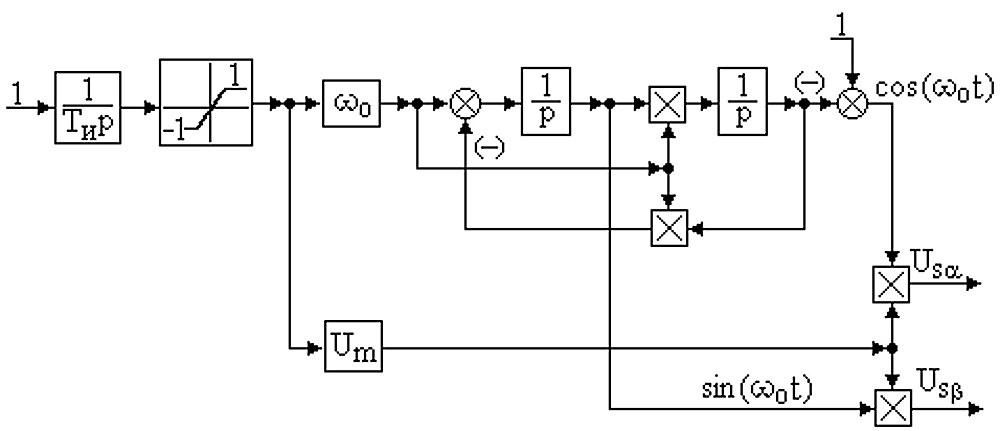
\includegraphics[width=0.8\linewidth]{img/inv-struct}}
            \caption{Структурная схема идеального преобразователя частоты}
            \label{fig:inv-struct}
        \end{figure}

        В структурной схеме рисунке \ref{fig:inv-struct} с помощью интегратора
        и блока ограничения построен задатчик интенсивности с единичным
        выходным сигналом. Собственно преобразователь частоты построен с
        помощью двух интеграторов и двух блоков умножения. На выходе первого
        интегратора получается синусоидальный сигнал с единичной амплитудой и
        переменной частотой $\omega_0$. На выходе второго интегратора
        получается сигнал вида $(1-\cos \omega_0 t)$. C помощью дополнительного
        сумматора эта функция вычитается из 1 и на выходе сумматора получается
        косинусоидальный сигнал с единичной амплитудой и переменной частотой
        $\omega_0$. Посредством второй пары умножителей единичные
        косинусоидальный и синусоидальный сигналы умножаются на амплитудное
        значение выходного напряжения преобразователя частоты $U_m$, также
        являющееся величиной переменной. Обе переменные величины, и частота
        $\omega_0$, и амплитуда $U_m$ формируются с помощью общего задатчика
        интенсивности, благодаря чему на выходах второй пары умножителей
        получаются эквивалентные напряжения статора асинхронного двигателя
        $U_{s\alpha}$ и $U_{s\beta}$ при реализации известного закона
        частотного управления $\frac{U_m}{\omega_0} = const$. 

        При необходимости динамическая модель идеального преобразователя
        частоты позволяет реализовать также любой другой закон частотного
        управления асинхронным двигателем. При создании модели асинхронного
        электропривода на основе преобразователей частоты с широтно-импульсной
        модуляцией идеализация преобразователя частоты не вносит существенных
        погрешностей в вычисления, так как токи и потокосцепления в таких
        системах практически синусоидальны.

    \subsection{Моделирование разомкнутой системы управления в программной
        среде MATLAB}

        Функциональная схема базовой системы частотного электропривода показана
        на рисунке \ref{fig:struct-old}. Математическая модель системы представлена на 
        рисунке \ref{fig:open-loop-model}. Результаты моделирования показаны на рисунках
        \ref{fig:open-loop-wm} - \ref{fig:open-loop-is_a}.

        По результатам моделирования можно сделать вывод от том, что
        разомкнутая система электропривода непригодна для использования в
        составе стенда исследования упругих колебаний, так как дает
        значительную просадку по скорости. Также система имеет неприемлемые
        динамические характеристики, что видно по скорости разгона
        электродвигателя.
        
        \begin{figure}[h!]
            \center{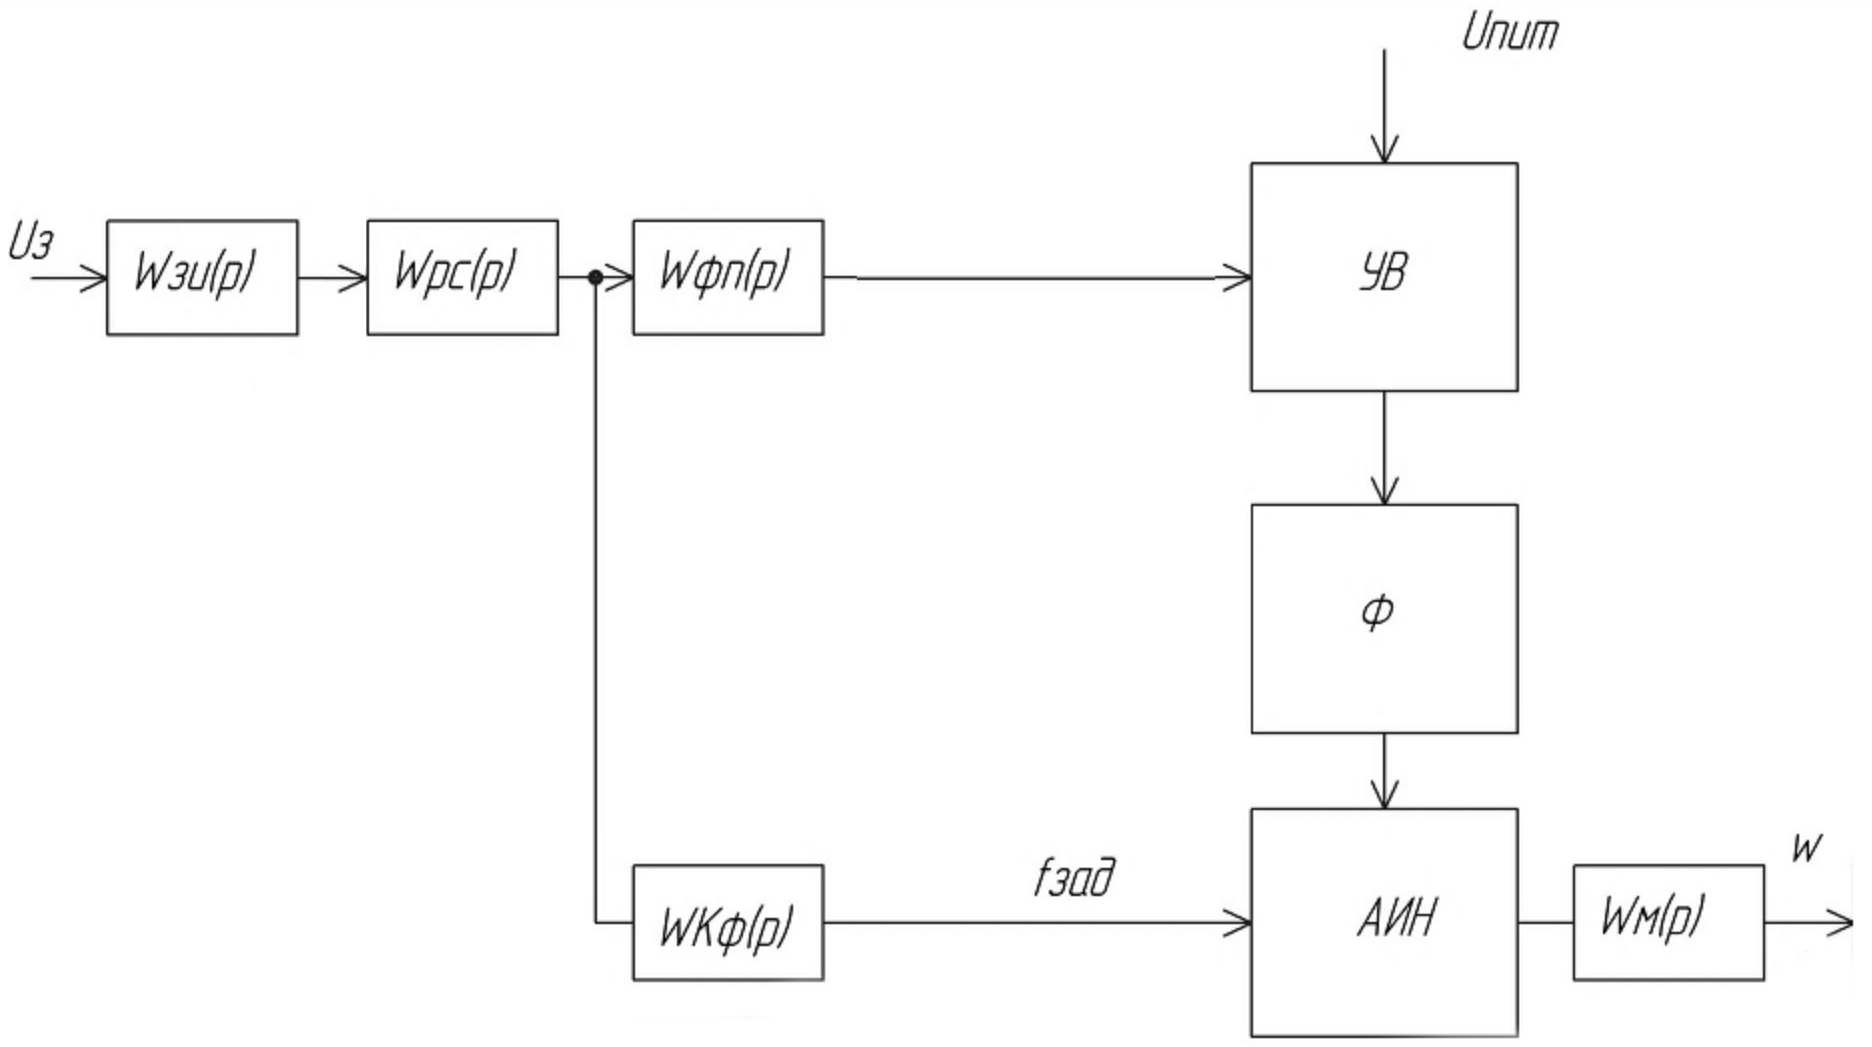
\includegraphics[width=0.8\linewidth]{img/struct-old}}
            \caption{Структурная схема разомкнутой системы электропривода с
                частотным преобразователем}
            \label{fig:struct-old}
        \end{figure}

        \begin{sidewaysfigure}
            \center{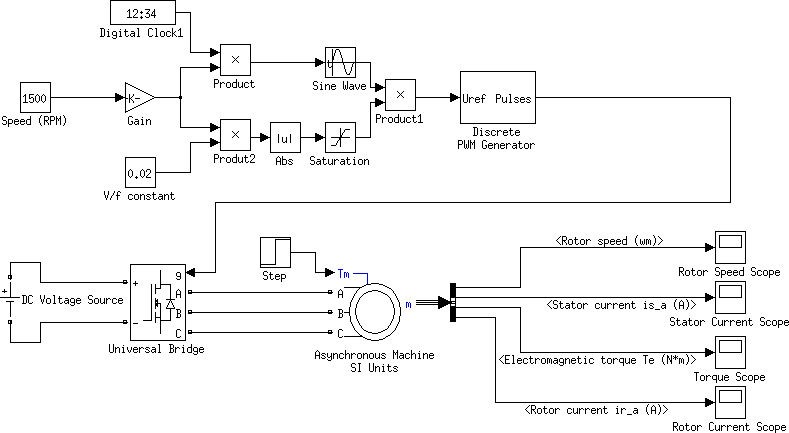
\includegraphics[width=1.0\linewidth]{img/open-loop-model}}
            \caption{Модель разомкнутой системы электропривода в MATLAB}
            \label{fig:open-loop-model}
        \end{sidewaysfigure}
        
        \begin{figure}[h!]
            \center{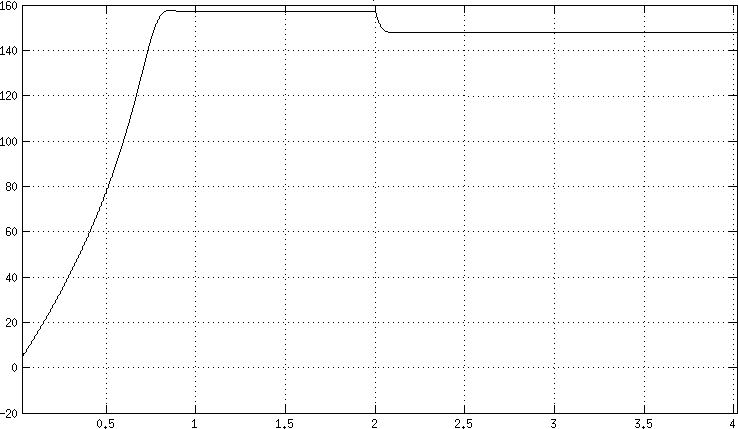
\includegraphics[width=0.95\linewidth]{img/open-loop-wm-fix}}
            \caption{График переходного процесса частоты вращения ротора
                разомкнутой системы}
            \label{fig:open-loop-wm}
        \end{figure}

        \begin{figure}[h!]
            \center{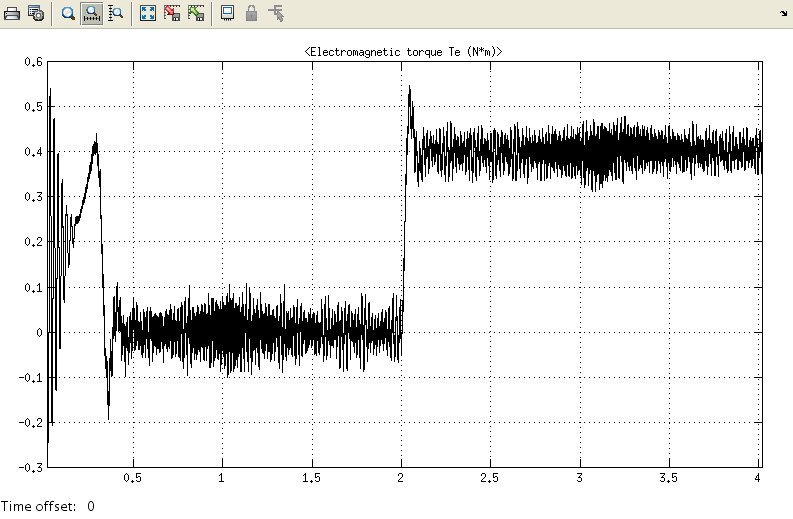
\includegraphics[width=0.95\linewidth]{img/open-loop-te}}
            \caption{График переходного процесса момента на валу двигателя в
                разомкнутой системе}
            \label{fig:open-loop-te}
        \end{figure}

        \begin{figure}[h!]
            \center{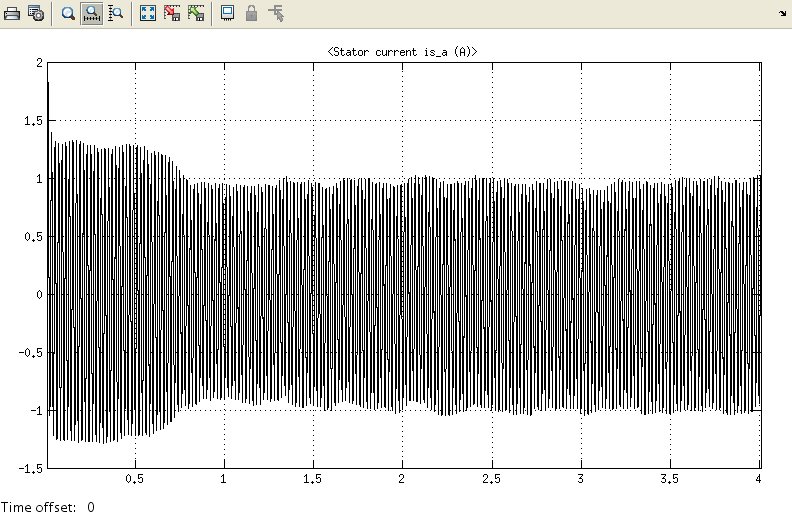
\includegraphics[width=1.0\linewidth]{img/open-loop-is_a}}
            \caption{График переходного процесса тока статора 
                разомкнутой системы}
            \label{fig:open-loop-is_a}
        \end{figure}

        %\afterpage{\clearpage}
        \clearpage
    
    \subsection{Моделирование системы управления с ПИД-регулятором скорости в
        программной среде MATLAB}

        Функциональная схема системы частотного электропривода с\\
        ПИД-регулятором скоростипоказана на рисунке \ref{fig:struct-new}.
        Математическая модель системы представлена на 
        рисунке \ref{fig:close-loop-model}. Результаты моделирования показаны на рисунках
        \ref{fig:close-loop-wm} - \ref{fig:close-loop-is_a}.

        Из графиков переходных процессов в системе электропривода с
        ПИД-регулированием скорости, можно сделать выводы о том, что система
        имеет лучшие динамические характеристики в сравнении с разомкнутой
        системой. Время выхода на установившийся режим после запуска двигателя
        сокращено более чем в два раза. Достигнута стабилизация скорости, что
        видно из графика переходного процесса частоты вращения   ротора.
        
        \begin{figure}[h!]
            \center{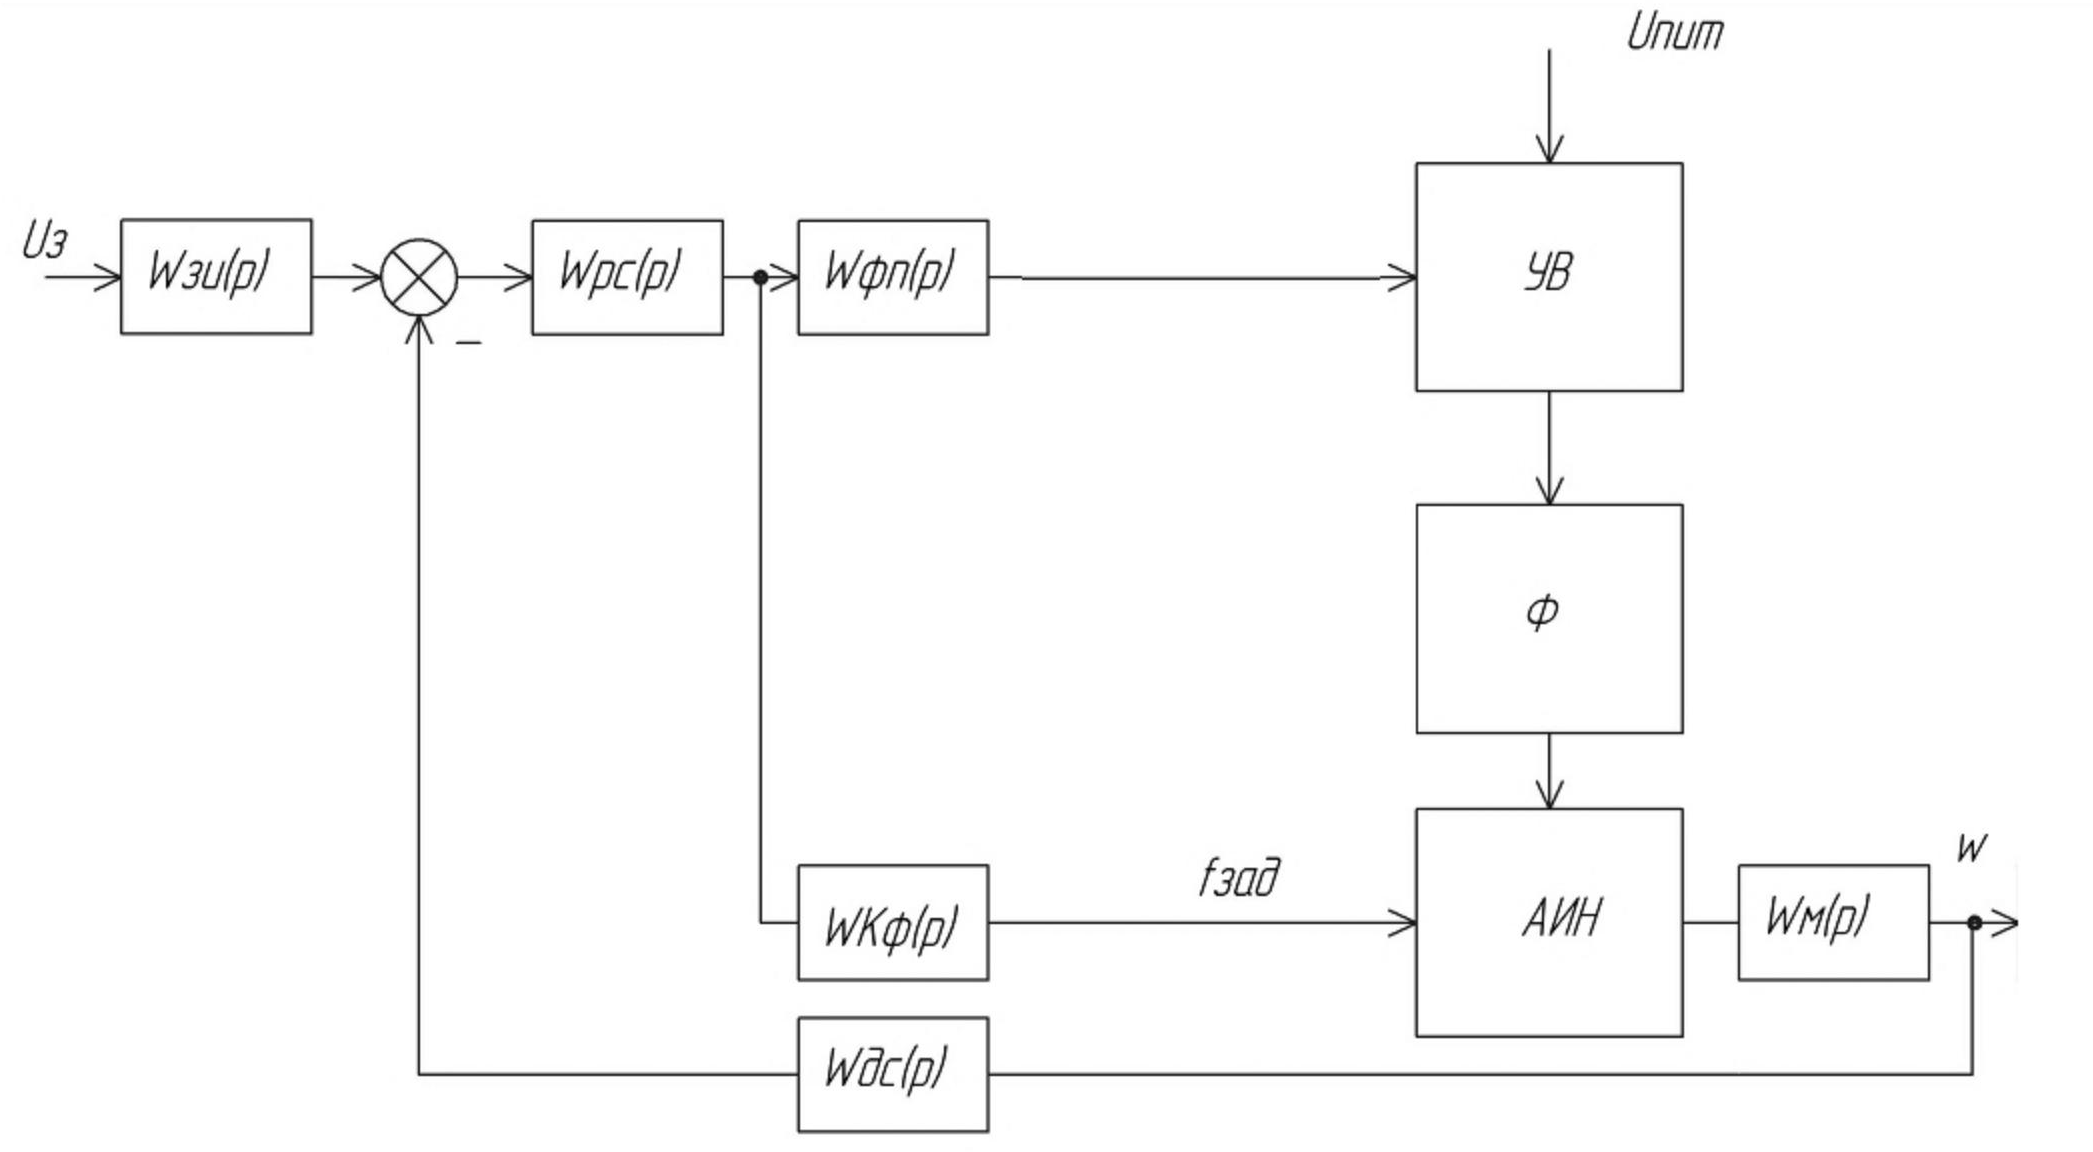
\includegraphics[width=0.8\linewidth]{img/struct-new}}
            \caption{Структурная схема замкнутой системы регулирования скорости
                электропривода с частотным преобразователем}
            \label{fig:struct-new}
        \end{figure}

        \begin{sidewaysfigure}
            \center{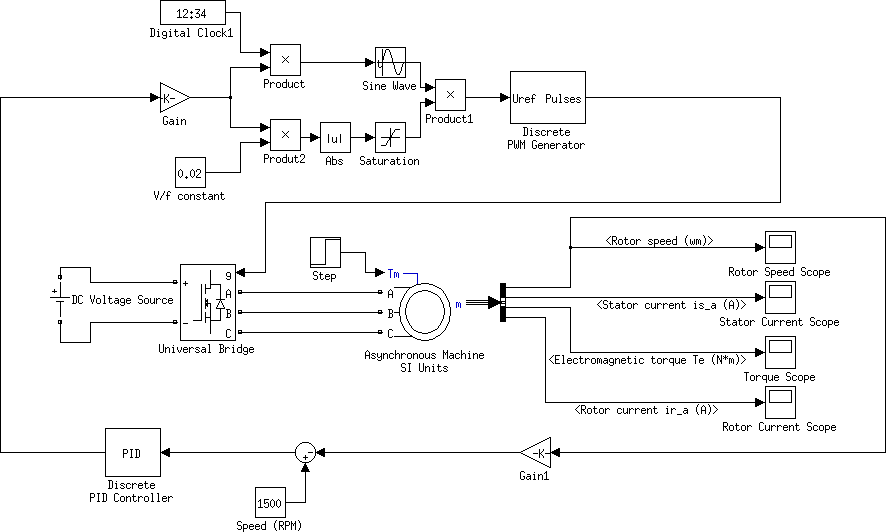
\includegraphics[width=1.0\linewidth]{img/close-loop-model}}
            \caption{Модель замкнутой системы электропривода в MATLAB}
            \label{fig:close-loop-model}
        \end{sidewaysfigure}
        
        \begin{figure}[h!]
            \center{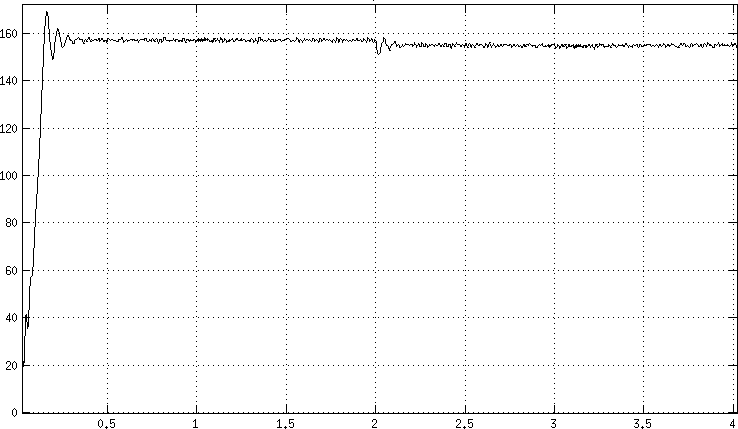
\includegraphics[width=0.9\linewidth]{img/close-loop-wm}}
            \caption{График переходного процесса частоты вращения ротора
                замкнутой системы}
            \label{fig:close-loop-wm}
        \end{figure}

        \begin{figure}[h!]
            \center{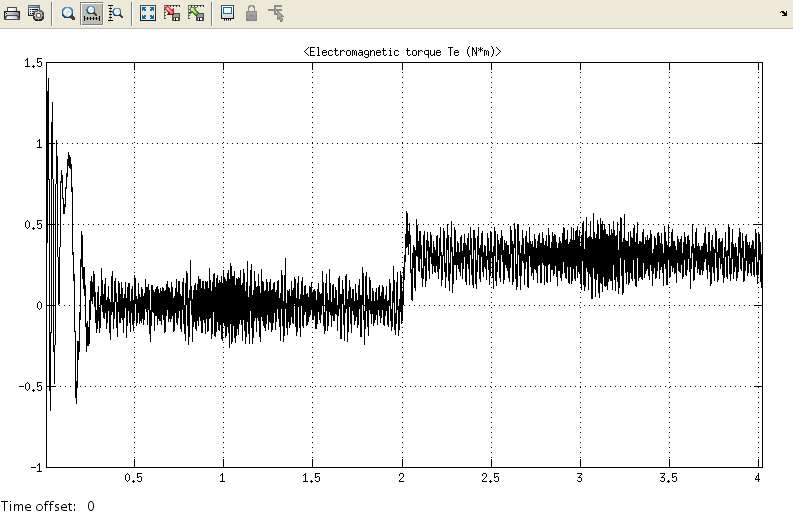
\includegraphics[width=0.9\linewidth]{img/close-loop-te}}
            \caption{График переходного процесса момента на валу двигателя в
                замкнутой системе}
            \label{fig:close-loop-te}
        \end{figure}

        \begin{figure}[h!]
            \center{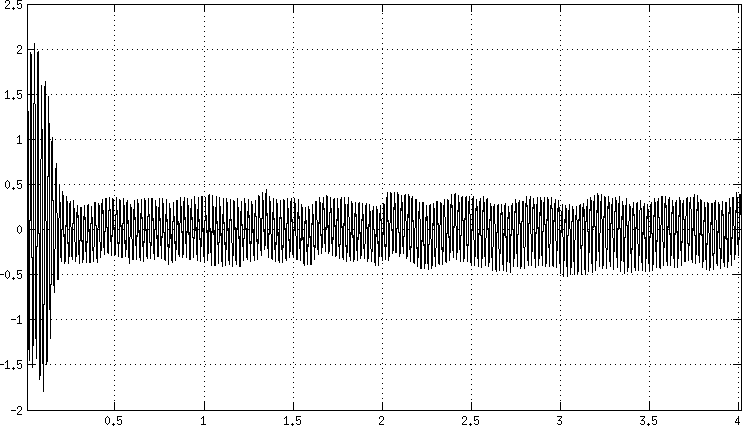
\includegraphics[width=1.0\linewidth]{img/close-loop-is_a}}
            \caption{График переходного процесса тока статора 
                замкнутой системы}
            \label{fig:close-loop-is_a}
        \end{figure}

        \clearpage

    \newpage

    % Специальная часть
    \section{Специальная часть}

    \newpage

    % Экономика
    \section{Экономическая часть}
    \subsection{Расчет капитальных затрат}
        В данном проекте проводилось проектирование и разработка автономного
        инвертора напряжения с реализацией закона поддержания постоянства
        соотношения U/f для управления асинхронным электроприводом.

        Спроектированный инвертор напряжения позволит проводить дальнейшие
        исследования и построение системы управления для демпфирования упругого
        соединения двигателя с инерционной массой. 

        В данном разделе приведен сравнительный расчет экономической
        эффективности разработанного инвертора напряжения с инвертором
        напряжении фирмы MOELLER. Следует учитывать также то, что при
        возможности серийного выпуска продукции ее себестоимость будет
        уменьшаться в зависимости от количества выпускаемой партии.

        Оценим экономическую целесообразность постройки стенда
        электромеханической системы асинхронного электропривода на основе
        разработанного частотного преобразователя, при этом в качестве базового
        варианта возьмем аналогичный по мощности частотный преобразователь
        MMX12 - 0,75 кВт фирмы MOELLER.

        В состав капитальных затрат системы электропривода входят: стоимость
        оборудования системы, стоимость резерва, строительно-монтажных работ, в
        том числе и заработная плата, транспортные расходы доставки
        оборудования, стоимость занимаемой площади здания,
        заготовительно-складские затраты.

        Определим стоимость оборудования установки базового варианта \\(таблица
        \ref{table:cost-base}).

        Определим стоимость оборудования установки нового варианта \\(таблица
        \ref{table:cost-new}).

        Стоимость резерва системы составляет 30\% от стоимости основного
        оборудования. Затраты на площадь помещения, где расположено
        оборудование, транспортные расходы, и заготовительно-складские затраты,
        принимают соответственно 15, 4 и 1,2\% от стоимости основного
        оборудования. Стоимость строительно-монтажных работ для данной системы
        составляет 10\% от стоимости основного оборудования (50\% этой суммы
        составляет заработная плата).

        \begin{longtable}{|p{8cm}|p{2,5cm}|p{2,5cm}|p{2,5cm}|}
        \caption{Стоимость оборудования
            базовой системы \label{table:cost-base}}\\
        \hline
        Наименование & Стоимость & Количество & Общая стоимость\\
        %\hline
        %1 & 2 & 3 & 4 \\
        \hline
        \endfirsthead
        \caption*{Продолжение таблицы
            \ref{table:cost-base}}\\
        \hline
        \endhead
        Частотный преобразователь MOELLER MX12 & 2700 грн & 1 шт & 2700 грн\\
        \hline
        Двигатель асинхронный АИР56А4У3 & 600 грн & 1 шт & 600 грн\\
        \hline
        Датчик положения ПДФ-5 & 500 грн & 2 шт & 1000 грн\\
        \hline
        \multicolumn{3}{|l|}{Общая сумма затрат на компоненты} & 4300 грн\\
        \hline
        \end{longtable}

        \begin{longtable}{|p{8cm}|p{2,5cm}|p{2,5cm}|p{2,5cm}|}
        \caption{Стоимость оборудования
            новой системы \label{table:cost-new}}\\
        \hline
        Наименование & Стоимость & Количество & Общая стоимость\\
        \hline
        1 & 2 & 3 & 4 \\
        \hline
        \endfirsthead
        \caption*{Продолжение таблицы
            \ref{table:cost-new}}\\
        \hline
        1 & 2 & 3 & 4 \\
        \endhead
        Конденсатор 10 мкФ 20 В & 0,20 грн & 5 шт. & 1 грн \\
        \hline
        Конденсатор 1000 мкФ 25 В & 1 грн & 1 шт. & 1 грн \\
        \hline
        Конденсатор 0,1 мкФ 50 В & 0,3 грн & 4 шт. & 1,2 грн \\
        \hline
        Конденсатор 0,01 мкФ 50 В & 0,3 грн & 6 шт. & 1,8 грн \\
        \hline
        Конденсатор 330 мкФ 450 В & 35 грн & 2 шт. & 70 грн \\
        \hline
        Реле 12V DC 16 A & 10 грн & 1 шт. & 10 грн \\
        \hline
        Резистор 0,25 Вт & 0,2 грн & 21 шт. & 4,2 грн \\
        \hline
        Резистор SMD 1206 & 0,1 грн & 35 шт. & 3,5 грн \\
        \hline
        Резистор 5 Вт & 1 грн & 2 шт. & 2 грн \\
        \hline
        Транзистор IRF740 & 6,5 грн & 7 шт. & 46 грн \\
        \hline
        ИМС IR2130 & 50 грн & 1 шт. & 50 грн \\
        \hline
        Диод FR106 & 0,2 грн & 10 шт. & 2 грн \\
        \hline
        Диод 1n4148 & 0,15 грн & 6 шт. & 0,9 грн \\
        \hline
        Стабилитрон 15 В 0,5 Вт & 0,5 грн & 6 шт & 3 грн \\
        \hline
        Мост диодный 35 А 1000 В & 15 грн & 1 шт & 15 грн \\
        \hline
        ИМС ADUM1300 & 35 грн & 3 шт & 105 грн \\
        \hline
        ИМС ADUM1201 & 17 грн & 1 шт & 17 грн \\
        \hline
        ИМС AT90PWM3 & 30 грн & 1шт & 40 грн \\
        \hline
        ИМС 74HC04 & 5 грн & 1шт & 5 грн \\
        \hline
        Провод монтажный & & & 15 грн\\
        \hline
        Стеклотекстолит фольгированный & & & 35 грн\\
        \hline
        Теплоотводящий радиатор  & 25 грн & 1 шт & 25 грн\\
        \hline
        Двигатель асинхронный АИР56А4У3 & 600 грн & 1 шт & 600 грн\\
        \hline
        Датчик положения ПДФ-5 & 500 грн & 2 шт & 1000 грн\\
        \hline
        \multicolumn{3}{|l|}{Общая сумма затрат на компоненты} & 2100 грн\\
        \hline
        \end{longtable}

        Рассчитаем капитальные затраты на оборудование для обоих вариантов:
        общая сумма оборудования базовой системы $Ц_{об} = 4300 \; \text{грн}$,
        модернизированной системы $Ц_{об} = 2060 \; \text{грн}$.

        Определим затраты на строительно-монтажные работы
        \begin{equation}
            S_\text{смр} = \text{Ц}_\text{об} \cdot 0,1.
        \end{equation}

        Определим заработную плату строительно-монтажных рабочих
        \begin{equation}
            S_\text{см} = S_\text{смр} \cdot 0,5.
        \end{equation}

        Определим общие затраты на оборудование
        \begin{equation}
            S_\text{об} = \text{Ц}_\text{об} + S_\text{см}. 
        \end{equation}

        Определим стоимость резерва системы
        \begin{equation}
            S_\text{рез} = \text{Ц}_\text{об} \cdot 0,3.
        \end{equation}

        Определим стоимость площади, занимаемую оборудованием
        \begin{equation}
            S_\text{пл} = \text{Ц}_\text{об} \cdot 0,15.
        \end{equation}

        Рассчитаем транспортные расходы на доставку оборудования
        \begin{equation}
            S_\text{тр} = \text{Ц}_\text{об} \cdot 0,04.
        \end{equation}

        Рассчитаем заготовительно-складские затраты
        \begin{equation}
            S_\text{зс} = \text{Ц}_{об} \cdot 0,012. 
        \end{equation}

        Рассчитаем общую сумму капитальных затрат
        \begin{equation}
            К = S_\text{об} + S_\text{рез} +
                S_\text{пл} + S_\text{тр} + S_\text{зс}. 
        \end{equation}

        Все расчеты проведем по вышеприведенным формулам и запишем в таблицу
        \ref{table:capital-cost}.

        \begin{longtable}{|p{8cm}|p{3cm}|p{4cm}|}
            \caption{Капитальные затраты на оборудование
                \label{table:capital-cost}}\\
            \hline
            Затраты & Базовая система & Модернизирован- ная система\\
            \hline
            \endfirsthead
            \caption*{Продолжение таблицы \ref{table:capital-cost}}\\
            \hline
            Затраты & Базовая система & Модернизирован- ная система\\
            \endhead
            \hline
            зарплата строительно-монтажных рабочих, грн & 215 & 105\\
            \hline
            затраты на оборудование, грн & 4515 & 2205\\
            \hline
            стоимость резерва, грн & 1290 & 630\\
            \hline
            стоимость площади, грн & 645 & 315\\
            \hline
            транспортные расходы, грн & 172 & 84\\
            \hline
            заготовительно-складские затраты, грн & 51,6 & 25,2\\
            \hline
            сумма капитальных затрат, грн & 6673,6 & 3259,2\\
            \hline
        \end{longtable}

    \subsection{Расчет эксплуатационных затрат}

        Эксплуатационные затраты определяются себестоимостью, которая состоит
        из:
        \begin{itemize}
            \item амортизационные отчисления;
            \item затраты на потребленную электроэнергию;
            \item затраты на ремонт оборудования;
            \item другие затраты.
        \end{itemize}

        Примем усредненную норму амортизации 8\% для всех объектов.

        Определим амортизационные отчисления
        \begin{equation}
            C_\text{а} = N_\text{а} \cdot \text{Ц}_\text{об}.
        \end{equation}

        Рассчитаем отчисления за площадь
        \begin{equation}
            C_\text{пл} = N_\text{а} \cdot S_\text{пл}.
        \end{equation}

        Рассчитаем полные амортизационные отчисления
        \begin{equation}
            C_\text{аПОЛ}  = C_\text{а} + C_\text{пл}.
        \end{equation}

        Проведем расчет эффективного фонда времени, при работе 12 часов в
        день, за год на складе
        \begin{equation}
            T_\text{эф} = 12 \cdot 365 = 4380 \; \text{ч}. 
        \end{equation}

        Рассчитаем расходы на потребляемую электроэнергию
        \begin{equation}
            C_\text{э} = \frac{P}{\eta} \cdot
                T_\text{эф} \cdot K_\text{в} \cdot K_\text{м} \cdot c ,
        \end{equation}

        где  $P$ – номинальная мощность используемого
            электродвигателя, кВт;\par
        $\eta$ – коэффициент полезного действия электрооборудования,
            доли;\par
        $T_\text{эф}$ – эффективный фонд времени работы, ч;\par
        $K_\text{в}$ – коэффициент использования по времени;\par
        $K_\text{м}$ – коэффициент использования по мощности;\par
        $C_\text{э}$ – стоимость 1 кВт ч электроэнергии, грн/кВт ч.\par

        Коэффициент полезного действия электрооборудования вычисляем как
        произведение коэффициентов полезного действия двигателя и
        преобразователя.  Для базового и нового вариантов коэффициент полезного
        действия равен 85\%.

        Коэффициент использования по времени для базового варианта равен 0,8.
        Коэффициент использования по мощности 0,67.

        Стоимость электроэнергии равна 0,45 грн/кВт ч.

        Эффективный фонд времени по обоим вариантам при работе в одну смену за
        год составит
        \begin{equation}
            T_\text{эф} = 8 \cdot 22 \cdot 12 = 2112 \; \text{ч}. 
        \end{equation}

        Рассчитаем затраты на текущий ремонт.

        Текущий ремонт электрооборудования производится на месте его установки
        с отключением от сети и остановкой силами сменного ремонтного
        персонала, обслуживающего данный агрегат (оборудование).  Затраты на
        текущий ремонт электрооборудования содержат следующие статьи:

        \begin{itemize}
            \item основная зарплата рабочих с начислениями $C_\text{зп}$;
            \item стоимость используемых материалов и комплектующих изделий
                $C_\text{м}$;
            \item цеховые и общезаводские расходы $C_\text{общ}$.
        \end{itemize}

        Для определения зарплаты рабочих-ремонтников необходимо знать
        трудоемкость ремонтных работ и эффективный фонд времени одного
        рабочего.  Трудоемкость ремонтных работ определяют из графика
        планово–предупредительных ремонтов.  Трудоемкость ремонтных работ
        составляет 25 чел–ч.  Эффективный фонд времени одного рабочего состоит
        из дней, оставшихся после вычитания из 365 календарных дней выходных и
        праздничных дней, а также дней, касающихся прочих невыходов на работу.
        Занятость по времени – 0,96. Эффективный фонд времени равен:
        \begin{equation}
            T = 8 \cdot (365 - 104) \cdot 0,96 = 2004,5 \; \text{ч}. 
        \end{equation}

        Заработная плата определяется через трудоемкость ремонтов и тарифную
        часовую ставку электромонтера, которая составляет 8 грн/ч.

        Тарифная зарплата
        \begin{equation}
            C_\text{зп}^T = 8 \cdot 25 = 200 \; \text{грн}. 
        \end{equation}

        К начислениям зарплаты относят премии (20\% от тарифной зарплаты),
        дополнительная зарплата (10\% от тарифной зарплаты), другие доплаты
        (10\% от тарифной зарплаты). В итоге начисления достигают 40\% от
        тарифной зарплаты.  Чтобы определить полную сумму выплат по зарплате
        рабочим, необходимо тарифную зарплату умножить на коэффициент 1,4.

        Таким образом, сумма полных выплат по зарплате
        \begin{equation}
            C_\text{зп} = C_\text{зп}^T \cdot 1,4,
        \end{equation}

        Затраты на материал и комплектующие изделия составляют
        \begin{itemize}
            \item при капитальном ремонте – 50\% от тарифной зарплаты;
            \item при среднем ремонте – 35\% от тарифной зарплаты;
            \item при текущем ремонте – 15\% от тарифной зарплаты.
        \end{itemize}

        В базовом варианте предусмотрены один капитальный ремонт, один средний
        и два текущих.

        Затраты на материалы и комплектующие будут равны
        \begin{equation}
            C_\text{м} = C_\text{зп}^T. 
        \end{equation}

        В смете годовых эксплуатационных расходов прочие расходы принимаются в
        размере 1\% от суммы капитальных вложений:
        \begin{equation}
            C_\text{пр.баз} = 0,01 \cdot K.
        \end{equation}

        Для анализа полученные данные запишем в таблицу (таблица
        \ref{table:usage-cost}).

        \begin{longtable}{|p{8cm}|p{3cm}|p{4cm}|}
            \caption{Эксплуатационные затраты
                \label{table:usage-cost}}\\
            \hline
            Затраты & Базовая система & Модернизирован- ная система\\
            \hline
            \endfirsthead
            \caption*{Продолжение таблицы \ref{table:usage-cost}}\\
            \hline
            Затраты & Базовая система & Модернизирован- ная система\\
            \endhead
            \hline
            Амортизационные отчисления, грн & 395,6 & 193\\
            \hline
            Затраты на электроэнергию, грн & 71 & 71\\
            \hline
            Заработная плата, грн & 280 & 280\\
            \hline
            Расходы на материалы, грн & 48 & 28\\
            \hline
            Общие расходы, грн & 143,5 & 117\\
            \hline
            Другие расходы, грн & 68 & 32\\
            \hline
            Всего эксплуатационных расходов, грн & 661 & 553\\
            \hline
        \end{longtable}
    
    \subsection{Расчет эффективности проектируемой системы}
        Так как величины капитальных вложений и эксплуатационных расходов при
        внедрении новой (усовершенствованной) системы электропривода станка
        стали меньше, чем при базовой системе, то для определения эффективности
        и целесообразности производимых изменений следует рассчитать
        сравнительные показатели.  
        
        Для сравнения эксплуатационных затрат используем показатель
        относительной экономии (уменьшения) затрат
        \begin{equation*}
            \lambda_\text{э} = 
                \frac{\text{Э}_\text{баз} - \text{Э}_\text{нов}}
                    {\text{Э}_\text{баз}} \cdot 100 \% = 
                        \frac{661-533}{661} \cdot 100 \% \approx 19 \%.
        \end{equation*}

        Приведенные затраты по базовому варианту составили
        \begin{equation*}
            \text{З}_\text{пр.баз} = 
                \text{Э}_\text{баз} + E_\text{н} \cdot K_\text{баз} = 
                    661 + 0,15 \cdot 6673,6 = 1662,04 \; \text{грн}.
        \end{equation*}

        По новому варианту
        \begin{equation*}
            \text{З}_\text{пр.нов} = 
                \text{Э}_\text{нов} + E_\text{н} \cdot K_\text{нов} = 
                    553 + 0,15 \cdot 3259,2 = 1021,88 \; \text{грн}.
        \end{equation*}

        Определим месячный экономический эффект
        \begin{equation*}
            \text{Э}_\text{м} = \text{Э}_\text{баз} 
                - \text{Э}_\text{нов} = 661 - 533 = 128 \; \text{грн}.
        \end{equation*}

        Срок окупаемости
        \begin{equation*}
            T_\text{o} = K_\text{нов}/(12 \cdot \text{Э}_\text{м})
                = 3259,2 / (12 \cdot 128) = 2,12 \; \text{года}.
        \end{equation*}

        Коэффициент эффективности капитальных вложении
        \begin{equation*}
            E = 1 / T_\text{о} = 1 / 2,12 = 0,47.
        \end{equation*}

       Расчетный коэффициент эффективности больше нормативного 
        \begin{equation*}
            E > E_\text{н},\qquad 0,47 > 0,15. 
        \end{equation*}

        Таким образом можно сделать вывод о том, что за счет более низкой
        стоимости капитальных затрат на построение частотного преобразователя в
        сравнении с затратами на использованием перобразователя выпускаемого
        промышленностью снижены эксплуатационные затраты на 19\%.
        Следовательно, по результатам вычислений, создание стенда на основе
        разработанного преобразователя экономически эффективно. Это
        подтверждается результатами технико-экономического обоснования,
        проведенного в данном дипломном проекте:
        \begin{itemize}
            \item имеем экономию капитальных вложений и эксплуатационных
                затрат;
            \item экономию электроэнергии благодаря правильному выбору ЭД в
                соответствии с режимом работы;
            \item повышение эффективности работы электродвигателя и как
                следствие снижение эксплуатационных расходов.
        \end{itemize}


    \newpage

    % Охрана труда
    \section{Охрана труда}

    \newpage

    % Заключение
    \section*{Заключение}
\addcontentsline{toc}{section}{Заключение}
        В настоящем проекте решается задача построения частотного асинхронного
        электропривода с широтно-импульсной модуляцией на основе
        микроконтроллера STM32F100RBT6B для лабораторно-исследовательского
        стенда. Также было выполнено моделирование данного электропривода.

        Разработана СУЭП с частотным регулированием скорости обеспечив
        оптимальные нагрузочные диаграммы и тахограммы. Для определения
        экономической целесообразности проекта был проведен расчет
        технико-экономических показателей.

        Был проведен анализ опасных и вредных производственных факторов при
        работе на данной установке, разработаны мероприятия по улучшению
        условий труда на рабочем месте и проанализированы возможные аварийные
        ситуаций для эффективного их устранения.

        Таким образом, спроектированная система обеспечивает все требования
        предъявленные в задании. 

    \newpage

    % Библиография
    \section*{Список литературы}
\addcontentsline{toc}{section}{Список литературы}


\end{document}
